\documentclass[]{book}
\usepackage{lmodern}
\usepackage{amssymb,amsmath}
\usepackage{ifxetex,ifluatex}
\usepackage{fixltx2e} % provides \textsubscript
\ifnum 0\ifxetex 1\fi\ifluatex 1\fi=0 % if pdftex
  \usepackage[T1]{fontenc}
  \usepackage[utf8]{inputenc}
\else % if luatex or xelatex
  \ifxetex
    \usepackage{mathspec}
  \else
    \usepackage{fontspec}
  \fi
  \defaultfontfeatures{Ligatures=TeX,Scale=MatchLowercase}
\fi
% use upquote if available, for straight quotes in verbatim environments
\IfFileExists{upquote.sty}{\usepackage{upquote}}{}
% use microtype if available
\IfFileExists{microtype.sty}{%
\usepackage{microtype}
\UseMicrotypeSet[protrusion]{basicmath} % disable protrusion for tt fonts
}{}
\usepackage[margin=1in]{geometry}
\usepackage{hyperref}
\hypersetup{unicode=true,
            pdftitle={A Minimal Book Example},
            pdfauthor={Yihui Xie},
            pdfborder={0 0 0},
            breaklinks=true}
\urlstyle{same}  % don't use monospace font for urls
\usepackage{natbib}
\bibliographystyle{apalike}
\usepackage{color}
\usepackage{fancyvrb}
\newcommand{\VerbBar}{|}
\newcommand{\VERB}{\Verb[commandchars=\\\{\}]}
\DefineVerbatimEnvironment{Highlighting}{Verbatim}{commandchars=\\\{\}}
% Add ',fontsize=\small' for more characters per line
\usepackage{framed}
\definecolor{shadecolor}{RGB}{248,248,248}
\newenvironment{Shaded}{\begin{snugshade}}{\end{snugshade}}
\newcommand{\KeywordTok}[1]{\textcolor[rgb]{0.13,0.29,0.53}{\textbf{#1}}}
\newcommand{\DataTypeTok}[1]{\textcolor[rgb]{0.13,0.29,0.53}{#1}}
\newcommand{\DecValTok}[1]{\textcolor[rgb]{0.00,0.00,0.81}{#1}}
\newcommand{\BaseNTok}[1]{\textcolor[rgb]{0.00,0.00,0.81}{#1}}
\newcommand{\FloatTok}[1]{\textcolor[rgb]{0.00,0.00,0.81}{#1}}
\newcommand{\ConstantTok}[1]{\textcolor[rgb]{0.00,0.00,0.00}{#1}}
\newcommand{\CharTok}[1]{\textcolor[rgb]{0.31,0.60,0.02}{#1}}
\newcommand{\SpecialCharTok}[1]{\textcolor[rgb]{0.00,0.00,0.00}{#1}}
\newcommand{\StringTok}[1]{\textcolor[rgb]{0.31,0.60,0.02}{#1}}
\newcommand{\VerbatimStringTok}[1]{\textcolor[rgb]{0.31,0.60,0.02}{#1}}
\newcommand{\SpecialStringTok}[1]{\textcolor[rgb]{0.31,0.60,0.02}{#1}}
\newcommand{\ImportTok}[1]{#1}
\newcommand{\CommentTok}[1]{\textcolor[rgb]{0.56,0.35,0.01}{\textit{#1}}}
\newcommand{\DocumentationTok}[1]{\textcolor[rgb]{0.56,0.35,0.01}{\textbf{\textit{#1}}}}
\newcommand{\AnnotationTok}[1]{\textcolor[rgb]{0.56,0.35,0.01}{\textbf{\textit{#1}}}}
\newcommand{\CommentVarTok}[1]{\textcolor[rgb]{0.56,0.35,0.01}{\textbf{\textit{#1}}}}
\newcommand{\OtherTok}[1]{\textcolor[rgb]{0.56,0.35,0.01}{#1}}
\newcommand{\FunctionTok}[1]{\textcolor[rgb]{0.00,0.00,0.00}{#1}}
\newcommand{\VariableTok}[1]{\textcolor[rgb]{0.00,0.00,0.00}{#1}}
\newcommand{\ControlFlowTok}[1]{\textcolor[rgb]{0.13,0.29,0.53}{\textbf{#1}}}
\newcommand{\OperatorTok}[1]{\textcolor[rgb]{0.81,0.36,0.00}{\textbf{#1}}}
\newcommand{\BuiltInTok}[1]{#1}
\newcommand{\ExtensionTok}[1]{#1}
\newcommand{\PreprocessorTok}[1]{\textcolor[rgb]{0.56,0.35,0.01}{\textit{#1}}}
\newcommand{\AttributeTok}[1]{\textcolor[rgb]{0.77,0.63,0.00}{#1}}
\newcommand{\RegionMarkerTok}[1]{#1}
\newcommand{\InformationTok}[1]{\textcolor[rgb]{0.56,0.35,0.01}{\textbf{\textit{#1}}}}
\newcommand{\WarningTok}[1]{\textcolor[rgb]{0.56,0.35,0.01}{\textbf{\textit{#1}}}}
\newcommand{\AlertTok}[1]{\textcolor[rgb]{0.94,0.16,0.16}{#1}}
\newcommand{\ErrorTok}[1]{\textcolor[rgb]{0.64,0.00,0.00}{\textbf{#1}}}
\newcommand{\NormalTok}[1]{#1}
\usepackage{longtable,booktabs}
\usepackage{graphicx,grffile}
\makeatletter
\def\maxwidth{\ifdim\Gin@nat@width>\linewidth\linewidth\else\Gin@nat@width\fi}
\def\maxheight{\ifdim\Gin@nat@height>\textheight\textheight\else\Gin@nat@height\fi}
\makeatother
% Scale images if necessary, so that they will not overflow the page
% margins by default, and it is still possible to overwrite the defaults
% using explicit options in \includegraphics[width, height, ...]{}
\setkeys{Gin}{width=\maxwidth,height=\maxheight,keepaspectratio}
\IfFileExists{parskip.sty}{%
\usepackage{parskip}
}{% else
\setlength{\parindent}{0pt}
\setlength{\parskip}{6pt plus 2pt minus 1pt}
}
\setlength{\emergencystretch}{3em}  % prevent overfull lines
\providecommand{\tightlist}{%
  \setlength{\itemsep}{0pt}\setlength{\parskip}{0pt}}
\setcounter{secnumdepth}{5}
% Redefines (sub)paragraphs to behave more like sections
\ifx\paragraph\undefined\else
\let\oldparagraph\paragraph
\renewcommand{\paragraph}[1]{\oldparagraph{#1}\mbox{}}
\fi
\ifx\subparagraph\undefined\else
\let\oldsubparagraph\subparagraph
\renewcommand{\subparagraph}[1]{\oldsubparagraph{#1}\mbox{}}
\fi

%%% Use protect on footnotes to avoid problems with footnotes in titles
\let\rmarkdownfootnote\footnote%
\def\footnote{\protect\rmarkdownfootnote}

%%% Change title format to be more compact
\usepackage{titling}

% Create subtitle command for use in maketitle
\newcommand{\subtitle}[1]{
  \posttitle{
    \begin{center}\large#1\end{center}
    }
}

\setlength{\droptitle}{-2em}
  \title{A Minimal Book Example}
  \pretitle{\vspace{\droptitle}\centering\huge}
  \posttitle{\par}
  \author{Yihui Xie}
  \preauthor{\centering\large\emph}
  \postauthor{\par}
  \predate{\centering\large\emph}
  \postdate{\par}
  \date{2017-12-19}

\usepackage{booktabs}
\usepackage{amsthm}
\makeatletter
\def\thm@space@setup{%
  \thm@preskip=8pt plus 2pt minus 4pt
  \thm@postskip=\thm@preskip
}
\makeatother

\begin{document}
\maketitle

{
\setcounter{tocdepth}{1}
\tableofcontents
}
\chapter{Prerequisites}\label{prerequisites}

This is a \emph{sample} book written in \textbf{Markdown}. You can use
anything that Pandoc's Markdown supports, e.g., a math equation
\(a^2 + b^2 = c^2\).

For now, you have to install the development versions of
\textbf{bookdown} from Github:

\begin{Shaded}
\begin{Highlighting}[]
\NormalTok{devtools}\OperatorTok{::}\KeywordTok{install_github}\NormalTok{(}\StringTok{"rstudio/bookdown"}\NormalTok{)}
\end{Highlighting}
\end{Shaded}

Remember each Rmd file contains one and only one chapter, and a chapter
is defined by the first-level heading \texttt{\#}.

To compile this example to PDF, you need to install XeLaTeX.

\chapter{Functions}\label{functions}

In this module, we'll explore how to use and create \textbf{functions}
in Python. Functions are the primary form of \emph{behavior abstraction}
in computer programming, and used to structure and generalize code
instructions. After considering a function in an abstract sense, we'll
look at how to use built-in Python functions, how to access additional
functions by importing Python modules, and finally how to write our own
functions.

\textbf{Contents}

\begin{itemize}
\tightlist
\item
  \protect\hyperlink{resources}{Resources}
\item
  \protect\hyperlink{what-are-functions}{What are Functions?}
\item
  \protect\hyperlink{python-function-syntax}{Python Function Syntax}
\item
  \protect\hyperlink{object-methods}{Object Methods}
\item
  \protect\hyperlink{built-in-python-functions}{Built-in Python
  Functions}
\item
  \protect\hyperlink{modules-and-libraries}{Modules and Libraries}
\item
  \protect\hyperlink{writing-functions}{Writing Functions}
\item
  \protect\hyperlink{doc-strings}{Doc Strings}
\end{itemize}

\hypertarget{resources}{\section{Resources}\label{resources}}

\begin{itemize}
\tightlist
\item
  \href{https://automatetheboringstuff.com/chapter3/}{Functions
  (Sweigart)}
\item
  \href{https://books.trinket.io/pfe/04-functions.html}{Functions
  (Severance)}
\item
  \href{http://openbookproject.net/thinkcs/python/english3e/fruitful_functions.html}{Fruitful
  Functions (Downey)} 
\end{itemize}

\hypertarget{what-are-functions}{\section{What are
Functions?}\label{what-are-functions}}

In a broad sense, a \textbf{function} is a named sequence of
instructions (lines of code) that you may want to perform one or more
times throughout a program. They provide a way of \emph{encapsulating}
multiple instructions into a single ``unit'' that can be used in a
variety of different contexts. So rather than needing to repeatedly
write down all the individual instructions for ``make a sandwich'' every
time you're hungry, you can define a \texttt{make\_sandwich()} function
once and then just \textbf{call} (execute) that function when you want
to perform those steps.

In addition to grouping instructions, functions in programming languages
like Python also follow the mathematical definition of functions, which
is a set of operations (instructions!) that are performed on some
\textbf{inputs} and lead to some \textbf{outputs}. Functions inputs are
called \textbf{arguments} or \textbf{parameters}, and we say that these
arguments are \textbf{passed} to a function (like a football). We say
that a function then \textbf{returns} an ouput for us to use.

\hypertarget{python-function-syntax}{\section{Python Function
Syntax}\label{python-function-syntax}}

Python functions are referred to by name (technically they are values
like any other variable). As in many programming languages, we
\textbf{call} a function by writing the name of the function followed
immediately (no space) by parentheses \texttt{()}. Inside the
parentheses, we put the \textbf{arguments} (inputs) to the function
separated by commas. Thus computer functions look just like mathematical
functions, but with names longer than \texttt{f()}.

\begin{Shaded}
\begin{Highlighting}[]
\CommentTok{# call the print() function, pass it "Hello world" value as an argument}
\BuiltInTok{print}\NormalTok{(}\StringTok{"Hello world"}\NormalTok{)  }\CommentTok{# "Hello world"}

\CommentTok{# call the str() function, pass it 598 as an argument}
\BuiltInTok{str}\NormalTok{(}\DecValTok{598}\NormalTok{)  }\CommentTok{# "598"}

\CommentTok{# call the len() function, pass it "python" as an argument}
\BuiltInTok{len}\NormalTok{(}\StringTok{"python"}\NormalTok{)  }\CommentTok{# 6 (the word is 6 letters long)}

\CommentTok{# call the round() function, pass it 3.1415 as the first arg and 2 as the second}
\CommentTok{# this is an example of a function that takes multiple (ordered) args}
\BuiltInTok{round}\NormalTok{(}\FloatTok{3.1415}\NormalTok{, }\DecValTok{2}\NormalTok{)  }\CommentTok{# 3.14, (3.1415 rounded to 2 decimal places)}

\CommentTok{# call the min() function, pass it 1, 6/8, AND 4/3 as arguments}
\CommentTok{# this is another example of a function that takes multiple args}
\BuiltInTok{min}\NormalTok{(}\DecValTok{1}\NormalTok{, }\DecValTok{6}\OperatorTok{/}\DecValTok{8}\NormalTok{, }\DecValTok{4}\OperatorTok{/}\DecValTok{3}\NormalTok{)  }\CommentTok{# 0.75, (6/8 is the smallest value)}
\end{Highlighting}
\end{Shaded}

\begin{itemize}
\tightlist
\item
  \emph{Note:} To keep functions and variables distinct, I try to always
  include empty parentheses \texttt{()} when referring to a function
  name. This does \emph{not} mean that the function takes no arguments,
  it is just a useful shorthand for indicating that something is a
  function rather than a variable.
\end{itemize}

Some functions (such as \texttt{min()} or \texttt{print()}) can be
passed as many arguments as you wish: \texttt{min()} will find the
minimum of \emph{all} the arguments, and \texttt{print()} will print
\emph{all} the arguments (in order), separated by a space:

\begin{Shaded}
\begin{Highlighting}[]
\CommentTok{# print() with 3 arguments instead of 1}
\BuiltInTok{print}\NormalTok{(}\StringTok{"I"}\NormalTok{, }\StringTok{"love"}\NormalTok{, }\StringTok{"programming"}\NormalTok{)  }\CommentTok{# "I love programming"}
\end{Highlighting}
\end{Shaded}

Besides ordered \textbf{positional arguments}, functions may also take
\textbf{keyword arguments}, which are arguments for specific function
inputs. These are written like variable assignments, but within the
function parameters:

\begin{Shaded}
\begin{Highlighting}[]
\CommentTok{# Use the `sep` keyword argument to specify the separator is '+++'}
\BuiltInTok{print}\NormalTok{(}\StringTok{"Hello"}\NormalTok{, }\StringTok{"World"}\NormalTok{, sep}\OperatorTok{=}\StringTok{'+++'}\NormalTok{)  }\CommentTok{# "Hello+++World"}
\end{Highlighting}
\end{Shaded}

Keyword arguments are always optional (they have ``default'' values,
like how the separator for \texttt{print()} defaults to a single space
\texttt{\textquotesingle{}\ \textquotesingle{}}). The default values are
specified in the function documentation (e.g., for
\href{https://docs.python.org/3/library/functions.html\#print}{\texttt{print()}}).

If you call any of these functions interactively (e.g., in an
interactvie shell or a Jupyter notebook), Python will display the
\textbf{returned value}. However, the computer is not able to ``read''
what is written to the console or an output cell---that's for humans to
view! If we want the computer to be able to \emph{use} a returned value,
we will need to give that value a name so that the computer can refer to
it. That is, we need to store the returned value in a variable:

\begin{Shaded}
\begin{Highlighting}[]
\CommentTok{# store min value in smallest_number variable}
\NormalTok{smallest_number }\OperatorTok{=} \BuiltInTok{min}\NormalTok{(}\DecValTok{1}\NormalTok{, }\DecValTok{6}\OperatorTok{/}\DecValTok{8}\NormalTok{, }\DecValTok{4}\OperatorTok{/}\DecValTok{3}\NormalTok{, }\DecValTok{5}\OperatorTok{+}\DecValTok{9}\NormalTok{)}

\CommentTok{# we can then use the variable as normal, such as mathematical operations}
\NormalTok{twice_min }\OperatorTok{=}\NormalTok{ smallest_number }\OperatorTok{*} \DecValTok{2}  \CommentTok{# 1.5}

\CommentTok{# we can use functions directly in expressions (the returned value is anonymous)}
\NormalTok{number }\OperatorTok{=}\NormalTok{ .}\DecValTok{5} \OperatorTok{*} \BuiltInTok{round}\NormalTok{(}\FloatTok{9.8}\NormalTok{)  }\CommentTok{# 5.0}

\CommentTok{# we can even pass the result of a function as an argument to another!}
\CommentTok{# watch out for where the parentheses close!}
\BuiltInTok{print}\NormalTok{(}\BuiltInTok{min}\NormalTok{(}\FloatTok{2.0}\NormalTok{, }\BuiltInTok{round}\NormalTok{(}\FloatTok{1.4}\NormalTok{)))  }\CommentTok{# prints 1}
\end{Highlighting}
\end{Shaded}

\hypertarget{object-methods}{\subsection{Object
Methods}\label{object-methods}}

In Python, all data values are \textbf{objects}, which are groups of
data (called \emph{attributes}) and behaviors---that is, information
about the value and the \emph{functions} that can be applied to that
data. For example, a Person object may have a name (e.g.,
\texttt{"Ada"}) and some behavior it can do to that data (e.g.,
\texttt{say\_name()}). Functions that are applied to an object's data
are also known as \textbf{methods}. We say that a method is \emph{called
on} that object.

While we'll discuss objects in more much detail later, for now we need
to understand that some functions are called \emph{on} particular
values. This is done using \textbf{dot notation}: you write the name of
the variable you wish to call the method on (i.e., apply the function
to), followed by a period (dot) \textbf{\texttt{.}}, followed by the
method name and arguments:

\begin{Shaded}
\begin{Highlighting}[]
\NormalTok{message }\OperatorTok{=} \StringTok{"Hello World"}

\CommentTok{# call the lower() method on the message to make a lowercase version}
\CommentTok{# Note that the original string does not change (strings are immutable)}
\NormalTok{lower_message }\OperatorTok{=}\NormalTok{ message.lower()  }\CommentTok{# "hello world"}

\CommentTok{# call the replace() method on the message}
\NormalTok{western_message }\OperatorTok{=}\NormalTok{ message.replace(}\StringTok{"Hello"}\NormalTok{, }\StringTok{"Howdy"}\NormalTok{)  }\CommentTok{# "Howdy World"}
\end{Highlighting}
\end{Shaded}

This is a common way of utilizing built-in Python functions.

\begin{itemize}
\tightlist
\item
  Note that dot notation is also used to access the \textbf{attributes}
  or \textbf{properties} of an object. So if a \texttt{Person} object
  has a \texttt{name} attribute, you would refer to that as
  \texttt{person.name}. In this sense, you can think of the \emph{dot
  operator} as being like the possessive \texttt{\textquotesingle{}s} in
  English: \texttt{person.name} refers so ``\texttt{person}**`s**
  \texttt{name}'``.
\end{itemize}

\hypertarget{built-in-python-functions}{\section{Built-in Python
Functions}\label{built-in-python-functions}}

As you may have noticed, Python comes with a large number of functions
that are built into the language. In the above examples, we used the
\texttt{print()} function to print a value to the console, the
\texttt{min()} function to find the smallest number among the arguments,
and the \texttt{round()} function to round to whole numbers. Similarly,
each data type in the language comes with their own set of methods: such
as the \texttt{lower()} and \texttt{replace()} methods on strings.

These functions are all described in the
\href{https://docs.python.org/3/index.html}{official documentation}. For
example, you can find a
\href{https://docs.python.org/3/library/functions.html}{list of built-in
functions} (though most of them will not be useful for us), as well as a
\href{https://docs.python.org/3/library/stdtypes.html\#string-methods}{list
of string methods}. To learn more about any individual function as well
as what functions are available, look it up in the documentation. You
can also use the \texttt{help()} function to look up the details of
other functions: \texttt{help(print)} will look up information on the
\texttt{print()} function.

\textbf{Important} ``Knowing'' how to program in a language is to some
extent simply ``knowing'' what provided functions are available in that
language. Thus you should look around and become familiar with these
functions\ldots{} but \emph{do not} feel that you need to memorize them!
It's enough to simply be aware ``oh yeah, there was a function that
rounded numbers'', and then be able to look up the name and arguments
for that function.

\hypertarget{modules-and-libraries}{\subsection{Modules and
Libraries}\label{modules-and-libraries}}

While Python has lots of built-in functions, many of them are not
immediately available for use. Instead, these functions are organized
into \textbf{modules}, which are collections of related functions and
variables. You must specifically load a module into your program in
order to access it's functions; this helps to reduce the amount of
memory that the Python interpreter needs to use in order to keep track
of all of the functions available.

You load a module (make it available to your program) by using the
\texttt{import} keyword, followed by the name of the module. This only
needs to be done once per script execution, and so is normally done at
the ``top'' of the script (in a Jupyter notebook, you can include an
``importing'' code cell, or import the module at the top of the cell in
which you first need it):

\begin{Shaded}
\begin{Highlighting}[]
\CommentTok{# load the math module, which contains mathematical functions}
\ImportTok{import}\NormalTok{ math}

\CommentTok{# call the math module's sqrt() function to calculate square root}
\NormalTok{math.sqrt(}\DecValTok{25}\NormalTok{)  }\CommentTok{# 5.0, (square root of 25)}

\CommentTok{# print out the math modules `pi` variable}
\BuiltInTok{print}\NormalTok{(math.pi)  }\CommentTok{# 3.141592653589793}
\end{Highlighting}
\end{Shaded}

Notice that we again use \textbf{dot notation} to call functions of a
particular module. Again, think of the \texttt{.} as a possessive
\texttt{\textquotesingle{}s} (``the \texttt{math} module\textbf{'s}
\texttt{sqrt} function'').

It is also possible to import only select functions or variables from a
module by using \texttt{from\ MODULE\ import\ FUNCTION}. This will load
the specific functions or variables into the \emph{global scope},
allowing you to call them without specifying the module:

\begin{Shaded}
\begin{Highlighting}[]
\CommentTok{# import the sqrt() function from the math module}
\ImportTok{from}\NormalTok{ math }\ImportTok{import}\NormalTok{ sqrt}

\CommentTok{# call the imported sqrt() function}
\NormalTok{sqrt(}\DecValTok{25}\NormalTok{)  }\CommentTok{# 5.0}

\CommentTok{# import multiple values by separating them with commas}
\ImportTok{from}\NormalTok{ math }\ImportTok{import}\NormalTok{ sin, cos pi}

\NormalTok{sin(pi}\OperatorTok{/}\DecValTok{2}\NormalTok{)  }\CommentTok{# 1.0}
\NormalTok{cos(pi}\OperatorTok{/}\DecValTok{2}\NormalTok{)  }\CommentTok{# 6.123233995736766e-17; 0 but with precision errors}

\CommentTok{# import everything from math}
\CommentTok{# this is useful for module with long or confusing names}
\ImportTok{from}\NormalTok{ math }\ImportTok{import} \OperatorTok{*}
\end{Highlighting}
\end{Shaded}

The collection of built-in modules such as \texttt{math} make up what is
called the \emph{standard library} of Python functions. However, it's
also possible to download and import additional modules written and
published by the Python community---what are known as \textbf{libraries}
or \textbf{packages}. Because many Python users encounter the same
challenges, programmers are able to benefit from the work of other and
\emph{reuse} solutions. This is the amazing thing about the open-source
community: people solve problems and then make those solutions available
to others.

A large number of additional libraries are included with the
\href{https://www.continuum.io/}{Anaconda} distribution you installed in
module 1. Anaconda also comes with a command-line utility
\href{https://conda.io/docs/}{\texttt{conda}} that can be used to easily
download and install new libraries. For example if you needed to install
Jupyter, you could use the command \texttt{conda\ install\ jupyter} from
the command-line.

\begin{itemize}
\tightlist
\item
  Python also comes with a command-line utility called
  \href{https://pip.pypa.io/en/stable/}{\texttt{pip}} for (``pip
  installs packages'') that can similarly be used to easily download and
  install packages. Note that you may need to set up a
  \href{http://python-guide-pt-br.readthedocs.io/en/latest/dev/virtualenvs/}{virtual
  environment} to effectively use \texttt{pip}; thus I recommend you
  rely on \texttt{conda} instead‐though the Anaconda package has
  everything you will need for this course.
\end{itemize}

\hypertarget{writing-functions}{\section{Writing
Functions}\label{writing-functions}}

Even more common than loading other peoples' functions is writing your
own. Functions are the primary way that we \emph{abstract} program
instructions, acting sort of like ``mini progams'' inside your larger
script. As Downey says:

\begin{quote}
Their primary purpose is to help us organize programs into chunks that
match how we think about the problem.
\end{quote}

Any time you want to organize your thinking---or if you have a task that
you want to repeat through the script---it's good practice to write a
function to perform that task. This will make your program easier to
understand and uilt, as well as limit repetition and reduce the
likelihood of error.

The best way to understand the syntax for defining a function is to look
at an example:

\begin{Shaded}
\begin{Highlighting}[]
\CommentTok{# A function named `MakeFullName` that takes two arguments}
\CommentTok{# and returns the "full name" made from them}
\KeywordTok{def}\NormalTok{ make_full_name(first_name, last_name):}
    \CommentTok{# Function body: perform tasks in here}
\NormalTok{    full_name }\OperatorTok{=}\NormalTok{ first_name }\OperatorTok{+} \StringTok{" "} \OperatorTok{+}\NormalTok{ last_name}

    \CommentTok{# Return: what you want the function to output}
    \ControlFlowTok{return}\NormalTok{ full_name}

\CommentTok{# Call the make_ful_name function with the values "Alice" and "Kim"}
\NormalTok{my_name }\OperatorTok{=}\NormalTok{ make_full_name(}\StringTok{"Alice"}\NormalTok{, }\StringTok{"Kim"}\NormalTok{)  }\CommentTok{# "Alice Kim"}
\end{Highlighting}
\end{Shaded}

Functions have a couple of pieces to them:

\begin{itemize}
\tightlist
\item
  \textbf{\texttt{def}}: Functions are defined by using the \texttt{def}
  keyword, which indicates that you are defining a function rather than
  a regular variable. This is followed by the \textbf{name} of the
  function, then a set of parentheses containing the arguments (Note
  that the \texttt{function\_name(arguments)} syntax mirrors how
  functions are called).
\end{itemize}

The line ends with a colon \textbf{\texttt{:}} which starts the function
body (see below).

\begin{itemize}
\tightlist
\item
  \textbf{Arguments}: The values put betweeen the parentheses in the
  function definition line are variables that \emph{will contain} the
  values passed in as \textbf{arguments}. For example, when we call
  \texttt{make\_full\_name("Alice","Kim")}, the value of the first
  argument (\texttt{"Alice"}) will be assigned to the first variable
  (\texttt{first\_name}), and the value of the second argument
  (\texttt{"Kim"}) will be assigned to the second variable
  (\texttt{last\_name}).
\end{itemize}

Importantly, we could have made the argument names anything we wanted
(\texttt{name\_first}, \texttt{given\_name}, etc.), just as long as we
then use \emph{that variable name} to refer to the argument while inside
the function. Moreover, these argument variable names \emph{only apply}
while inside the function (they are \textbf{scoped} to the function).
You can think of them like ``nicknames'' for the values. The variables
\texttt{first\_name}, \texttt{last\_name}, and \texttt{full\_name} only
exist within this particular function.

Note that a function may have no arguments, causing the parenthese to be
empty:

\texttt{python\ \ \ def\ say\_hello():\ \ \ \ \ \ \ print("Hello\ world!")}

You can give a function \emph{keyword arguments} by assigning a default
value to the argument in the function definition:

```python \# includes a single keyword argument def greet(greeting =
``Hello''): print(greeting + " world``)

\# call by assigning to the arg greet(greeting = ``Hi'') \# ``Hi world''

\# call wihout assigning an argument, using the default value greet() \#
``Hello world'' ```

\begin{itemize}
\item
  \textbf{Body}: The body of the function is a \textbf{block} of code.
  The funcion definition ends with a colon \textbf{\texttt{:}} to
  indicate that it is followed by a \emph{block}, which is a list of
  Python statements (lines of code). Which statements are part of the
  block are indicated by \emph{indentation}: statements are indented by
  4 spaces to make them part of that particular block. A block can
  contain as many lines of code as you want---you'll usually want more
  than 1 to make a function workwhile, but if you have more than 20 you
  might want to break your code up into separate functions. You can use
  the argument variables in here, create new variables, call other
  functions\ldots{} basically any code that you would write outside of a
  function can be written inside of one as well!
\item
  \textbf{Return value}: You can specify what output a function produces
  by using the \textbf{\texttt{return}} keyword, followed by the value
  that you wish \emph{your function} to return (output). A
  \texttt{return} statement will end the current function and
  \emph{return} the flow of code execution to whereever this function
  was called from. Note that even though we returned a variable called
  \texttt{full\_name}, that variable was \emph{local} to the function
  and so doesn't exist outside of it; thus we have to take the returned
  value and assign it to a new variable (as with
  \texttt{my\_name\ =\ make\_full\_name("Alice",\ "Kim")}).
\end{itemize}

Because the \texttt{return} statement exits the function, it is almost
always the last line of code in the function; any statements after a
\texttt{return} statement will not be run!

\begin{itemize}
\tightlist
\item
  A function does not need to return a value (as in the
  \texttt{say\_helo()} example above). In this case, omit the
  \texttt{return} statement.
\end{itemize}

We can call (execute) a function we defined the same way we called
built-in functions. When we do so, Python will take the
\textbf{arguments} we passed in (e.g., \texttt{"Alice"} and
\texttt{"Kim"}) and assign them to the \emph{argument variables}. Then
the interpreter executes each line of code in the \textbf{function body}
one at a time. When it gets to the \texttt{return} statement, it will
end the function and return the given value, which can then be assigned
to a different variable (outside of the function).

\hypertarget{doc-strings}{\subsection{Doc Strings}\label{doc-strings}}

We create new functions as ways of \emph{abstracting} behavior, in order
to make programs easier to read and understand. Thus it is important to
be clear about the purpose and use of any functions you create. This can
partially done through effective function and argument names:
\texttt{def\ calc\_rectangle\_area(width,\ height)} is pretty
self-explanatory, whereas \texttt{def\ func(a,b,c)} isn't).

\begin{itemize}
\tightlist
\item
  \emph{Style requirement:} Name functions as phrases starting with
  \emph{verbs} (because function do things), and variables as nouns.
\end{itemize}

Nevertheless, in order to make sure that functions are as clear as
possible, you should include \textbf{documentation} in the form of a
\emph{comment} that describes in plain English what a function does: its
inputs (arguments) once, output (return value), and overall behavior. In
Python we document functions by providing a \textbf{doc string}. This is
a string literal (written in multi-line triple quotes \texttt{"""})
placed immediately below the function declaration:

\begin{Shaded}
\begin{Highlighting}[]
\KeywordTok{def}\NormalTok{ to_celcius(degrees_farenheit):}
    \CommentTok{"""Converts the given degrees (in Farenheit) to degrees in celcius, and}
\CommentTok{       returns the result.}
\CommentTok{    """}
\NormalTok{    celcius }\OperatorTok{=}\NormalTok{ (degrees_farenheit }\OperatorTok{-} \DecValTok{32}\NormalTok{)}\OperatorTok{*}\NormalTok{(}\DecValTok{5}\OperatorTok{/}\DecValTok{9}\NormalTok{)}
    \ControlFlowTok{return}\NormalTok{ celcius}
\end{Highlighting}
\end{Shaded}

\begin{itemize}
\item
  Note that this string isn't assigned to a variable; it is treated as a
  valid statement because it is immediately below the function
  declaration.
\item
  You can view the doc string by calling the \texttt{help()} function
  with your function's name as the parameter! In fact, when you call
  \texttt{help()} on any built-in function, what you are viewing is that
  function's doc string.
\end{itemize}

Doc strings should include the following information:

\begin{enumerate}
\def\labelenumi{\arabic{enumi}.}
\tightlist
\item
  What the function does \emph{from the perspective of someone who would
  call the function}. This should be a short (1-2 sentence) summary;
  don't describe the individual instructions that are executed, but an
  \emph{abstraction} of the code's purpose.
\end{enumerate}

\begin{itemize}
\tightlist
\item
  If you mention variables, operations, functions, or control
  structures, your comment isn't at a high enough level of abstraction!
\end{itemize}

\begin{enumerate}
\def\labelenumi{\arabic{enumi}.}
\setcounter{enumi}{1}
\item
  Descriptions of the expected arguments. Clarify any ambiguities in
  type (e.g., a number or a string) and units.
\item
  Description of the returned value (if any). Explain the meaning, type
  (e.g., number or string), etc.
\end{enumerate}

It's good to think of doc strings as defining a ``contract'': you are
specifying that ``if you give the function this set of inputs, it will
perform this behavior and give you this output.''.

For simple methods you can build this information into a single sentence
as in the above example. But for more complex functions, you may need to
use a more complex format for your doc string. See the
\href{http://google.github.io/styleguide/pyguide.html?showone=Comments\#Comments}{Google
Style Guide} for an example.

\chapter{Logic and Conditionals}\label{logic-and-conditionals}

Programming involves writing instructions for a computer to execute.
However, what allows computer programs to be most useful is when they
are able to \emph{decide which} instructions instructions to execute
based on a particular situation. This is refered to as code branching,
and is used to shape the
\href{https://en.wikipedia.org/wiki/Control_flow}{flow of control} of
the computer code. In this module, you will learn how to utilize
\textbf{conditional statements} in order to include control flow in your
Python scripts.

\textbf{Contents}

\begin{itemize}
\tightlist
\item
  \protect\hyperlink{resources}{Resources}
\item
  \protect\hyperlink{booleans}{Booleans}
\item
  \protect\hyperlink{boolean-operators}{Boolean Operators}
\item
  \protect\hyperlink{conditional-statements}{Conditional Statements}
\item
  \protect\hyperlink{designing-conditions}{Designing Conditions}
\item
  \protect\hyperlink{modules-vs-scripts}{Modules vs.~Scripts}
\end{itemize}

\section{Resources}\label{resources-1}

\begin{itemize}
\tightlist
\item
  \href{https://books.trinket.io/pfe/03-conditional.html}{Conditional
  Execution (Downey)}
\item
  \href{http://openbookproject.net/thinkcs/python/english3e/conditionals.html}{Conditionals
  (Severance)}
\item
  \href{https://automatetheboringstuff.com/chapter2/}{Flow Control
  (Sweigart)} (first half)
\end{itemize}

\hypertarget{booleans}{\section{Booleans}\label{booleans}}

In addition to the basic data types \texttt{int}, \texttt{float}, and
\texttt{str}, Python supports a \emph{logical} data type called a
\textbf{Boolean} (class \texttt{bool}). A boolean represents
``yes-or-no'' data, and can be exactly one of two values: \texttt{True}
or \texttt{False} (note the capitalization). Importantly, these
\textbf{are not} the Strings \texttt{"True"} and \texttt{"False"};
boolean values are a different type!

\begin{Shaded}
\begin{Highlighting}[]
\BuiltInTok{type}\NormalTok{(}\VariableTok{True}\NormalTok{)    }\CommentTok{# <class 'bool'>}
\BuiltInTok{type}\NormalTok{(}\StringTok{"True"}\NormalTok{)  }\CommentTok{# <class 'str'>}
\BuiltInTok{type}\NormalTok{(true)    }\CommentTok{# NameError: name 'true' is not defined}
              \CommentTok{# e.g., no variable called `true`!}
\end{Highlighting}
\end{Shaded}

\begin{itemize}
\tightlist
\item
  \emph{Fun fact}: logical values are called ``booleans'' after
  mathematician and logician
  \href{https://en.wikipedia.org/wiki/George_Boole}{George Boole}, who
  invented many of the rules and uses of this construction (called
  \href{https://en.wikipedia.org/wiki/Boolean_algebra}{Boolean
  algebra}).
\end{itemize}

Boolean values are most commonly the result of applying a
\textbf{relational operator} (also called a \textbf{comparison
operator}) to some other data type. Comparison operators are used to
compare values and include: \texttt{\textless{}} (less than),
\texttt{\textgreater{}} (greater than), \texttt{\textless{}=}
(less-than-or-equal, written as read), \texttt{\textgreater{}=}
(greater-than-or-equal, written as read), \texttt{==} (equal), and
\texttt{!=} (not-equal).

\begin{Shaded}
\begin{Highlighting}[]
\NormalTok{x }\OperatorTok{=} \DecValTok{3}
\NormalTok{y }\OperatorTok{=} \FloatTok{3.15}

\CommentTok{# compare numbers}
\NormalTok{x }\OperatorTok{>}\NormalTok{ y  }\CommentTok{# returns logical value False ("x is bigger than y" is a False statement)}
\NormalTok{y }\OperatorTok{!=}\NormalTok{ x  }\CommentTok{# returns logical value True ("y is not-equal to x" is a True statement)}

\CommentTok{# compare x to pi (built-in variable)}
\NormalTok{y }\OperatorTok{==}\NormalTok{ math.pi  }\CommentTok{# returns logical value False}

\CommentTok{# compare strings (based on alphabetical ordering)}
\CommentTok{"cat"} \OperatorTok{>} \StringTok{"dog"}  \CommentTok{# returns False}
\end{Highlighting}
\end{Shaded}

\begin{itemize}
\tightlist
\item
  \textbf{Important} \texttt{==} (two equals signs) is a comparison
  operator, but \texttt{=} (one equals sign) is the assignment operator!
\end{itemize}

Note that boolean variables should be named as \emph{statements of
truth}. Use words such as \texttt{is} in the variable name:

\begin{Shaded}
\begin{Highlighting}[]
\NormalTok{is_early }\OperatorTok{=} \VariableTok{True}
\NormalTok{is_sleeping }\OperatorTok{=} \VariableTok{False}
\NormalTok{needs_coffee }\OperatorTok{=} \VariableTok{True}
\end{Highlighting}
\end{Shaded}

\hypertarget{boolean-operators}{\subsection{Boolean
Operators}\label{boolean-operators}}

In addition, boolean values support their own operators (called
\textbf{logical operators} or \textbf{boolean operators}). These
operators are applied to boolean values and produce boolean values, and
allow you to make more complex \emph{boolean expressions}:

\begin{itemize}
\tightlist
\item
  \textbf{\texttt{and}} (conjunction) produces \texttt{True} if both of
  the operands are \texttt{True}, and \texttt{False} otherwise
\item
  \textbf{\texttt{or}} (disjunction) produces \texttt{True} if
  \emph{either} of the operands are \texttt{True}, and \texttt{False}
  otherwise
\item
  \textbf{\texttt{not}} (negation) is a
  \href{https://en.wikipedia.org/wiki/Unary_operation}{unary operator}
  that produces \texttt{True} if the operand is \texttt{False}, and
  \texttt{False} otherwise
\end{itemize}

\begin{Shaded}
\begin{Highlighting}[]
\NormalTok{x }\OperatorTok{=} \FloatTok{3.1}
\NormalTok{y }\OperatorTok{=} \FloatTok{3.2}

\CommentTok{# Assign bool values to variables}
\NormalTok{x_less_than_pi }\OperatorTok{=}\NormalTok{ x }\OperatorTok{<}\NormalTok{ math.pi  }\CommentTok{# True}
\NormalTok{y_less_than_pi }\OperatorTok{=}\NormalTok{ y }\OperatorTok{<}\NormalTok{ math.pi  }\CommentTok{# False}

\CommentTok{# boolean operators}
\NormalTok{x_less_than_pi }\KeywordTok{and}\NormalTok{ y_less_than_pi  }\CommentTok{# False}
\NormalTok{x_less_than_pi }\KeywordTok{or}\NormalTok{ y_less_than_pi  }\CommentTok{# True}

\CommentTok{# this works because Python is amazing}
\NormalTok{x }\OperatorTok{<}\NormalTok{ math.pi }\OperatorTok{<}\NormalTok{ y  }\CommentTok{# True}


\NormalTok{pet }\OperatorTok{=} \StringTok{"dog"}

\CommentTok{# it is NOT the case that pet is "cat"}
\KeywordTok{not}\NormalTok{ pet }\OperatorTok{==} \StringTok{"cat"}  \CommentTok{# True}

\CommentTok{# pet is "cat" OR "dog"}
\NormalTok{pet }\OperatorTok{==} \StringTok{"cat"} \KeywordTok{or}\NormalTok{ pet }\OperatorTok{==} \StringTok{"dog"}  \CommentTok{# True}

\CommentTok{# this doesn't work (operators are applied left-to-right; check the types!)}
\CommentTok{# see "short-circuiting" below, as well as http://stackoverflow.com/a/19213583}
\NormalTok{pet }\OperatorTok{==} \StringTok{"cat"} \KeywordTok{or} \StringTok{"dog"}  \CommentTok{# "dog"}
\end{Highlighting}
\end{Shaded}

Because boolean expressions produce \emph{more} booleans, it is possible
to combine these into complex logical expressions:

\begin{Shaded}
\begin{Highlighting}[]
\CommentTok{# given two booleans P and Q}
\NormalTok{P }\OperatorTok{=} \VariableTok{True}
\NormalTok{Q }\OperatorTok{=} \VariableTok{False}

\NormalTok{P }\KeywordTok{and} \KeywordTok{not}\NormalTok{ Q  }\CommentTok{# True}
\KeywordTok{not}\NormalTok{ P }\KeywordTok{and}\NormalTok{ Q  }\CommentTok{# False}
\KeywordTok{not}\NormalTok{ (P }\KeywordTok{and}\NormalTok{ Q)  }\CommentTok{# True}
\NormalTok{(}\KeywordTok{not}\NormalTok{ P) }\KeywordTok{or}\NormalTok{ (}\KeywordTok{not}\NormalTok{ Q)  }\CommentTok{# True}
\end{Highlighting}
\end{Shaded}

The last two expressions in the above example are equivalent logical
statements for \emph{any} combination of values for \texttt{P} and
\texttt{Q}, what is known as
\href{https://en.wikipedia.org/wiki/De_Morgan\%27s_laws}{De Morgan's
Laws}. Indeed, many logical statements can be written in multiple
equivalent ways.

Finally, note that when using an \texttt{and} operator, Python will
\textbf{short-circuit} the second operand and never evaluate it if the
first is found to be \texttt{False} (after all, if the first operand
isn't \texttt{True} there is no way for the entire \texttt{and}
expression to be!)

\begin{Shaded}
\begin{Highlighting}[]
\NormalTok{x }\OperatorTok{=} \DecValTok{2}
\NormalTok{y }\OperatorTok{=} \DecValTok{0}
\NormalTok{x }\OperatorTok{==} \DecValTok{2} \KeywordTok{and}\NormalTok{ x}\OperatorTok{/}\NormalTok{y }\OperatorTok{>} \DecValTok{1}  \CommentTok{# ZeroDivisionError: division by zero}
\NormalTok{x }\OperatorTok{==} \DecValTok{3} \KeywordTok{and}\NormalTok{ x}\OperatorTok{/}\NormalTok{y }\OperatorTok{>} \DecValTok{1}  \CommentTok{# no error (short-circuited)}

\CommentTok{# Use a "guardian expression" (make sure y is not 0)}
\CommentTok{# to avoid any errors}
\NormalTok{y }\OperatorTok{!=} \DecValTok{0} \KeywordTok{and}\NormalTok{ x}\OperatorTok{/}\NormalTok{y }\OperatorTok{>} \DecValTok{1}  \CommentTok{# no error (short-circuited)}
\end{Highlighting}
\end{Shaded}

\begin{itemize}
\tightlist
\item
  The reason this works is because Python interpreter reads the
  expression \texttt{P\ and\ Q}, it produces \texttt{Q} if \texttt{P} is
  \texttt{True}, and \texttt{P} otherwise. This is because if \texttt{P}
  is \texttt{True}, then the overall truth of the expression is
  dependent entirely on \texttt{Q} (and thus that can just be returned).
  Similarly, if \texttt{P} is \texttt{False}, then the whole statement
  is false (equivalent to \texttt{P}!)
\end{itemize}

\hypertarget{conditional-statements}{\section{Conditional
Statements}\label{conditional-statements}}

One of the primary uses of Boolean values (and the \emph{boolean
expressions} that produce them) is to control the flow of execution in a
program (e.g., what lines of code get run in what order). While we can
use \emph{functions} are able to organization instructions, we can also
have our program decide which set of instructions to execute based on a
set of conditions. These deciisions are specified using
\textbf{conditional statements}.

In an abstract sense, an conditional statement is saying:

\begin{verbatim}
IF something is true
  do some lines of code
OTHERWISE
  do some other lines of code
\end{verbatim}

In Python, we write these conditional statements using the keywords
\textbf{\texttt{if}} and \textbf{\texttt{else}} and the following
syntax:

\begin{Shaded}
\begin{Highlighting}[]
\ControlFlowTok{if}\NormalTok{ condition:}
    \CommentTok{# lines of code to run if condition is True}
\ControlFlowTok{else}\NormalTok{:}
    \CommentTok{# lines of code to run if condition is False}
\end{Highlighting}
\end{Shaded}

The \textbf{\texttt{condition}} can be any Boolean value (or any
expression that evaluates to a boolean value). Both the
\textbf{\texttt{if}} statement and \textbf{\texttt{else}} clause are
followed by a colon \textbf{\texttt{:}} and a \textbf{block}, which is a
set of \emph{indented} statements to run (similar to the blocks used in
functions). It is also possible to \emph{omit} the \texttt{else}
statement and its block if there are no instructions to run in the
``otherwise'' situation:

\begin{Shaded}
\begin{Highlighting}[]
\NormalTok{porridge_temp =}\StringTok{ }\DecValTok{115}  \CommentTok{# temperature in degrees F}

\ControlFlowTok{if}\NormalTok{ porridge_temp }\OperatorTok{>}\StringTok{ }\DecValTok{120}\OperatorTok{:}
\StringTok{    }\KeywordTok{print}\NormalTok{(}\StringTok{"This porridge is too hot!"}\NormalTok{)}
\ControlFlowTok{else}\OperatorTok{:}
\StringTok{    }\KeywordTok{print}\NormalTok{(}\StringTok{"This porridge is NOT too hot!"}\NormalTok{)}

\NormalTok{too_cold =}\StringTok{ }\NormalTok{porridge_temp }\OperatorTok{<}\StringTok{ }\DecValTok{70}  \CommentTok{# a boolean variable}
\ControlFlowTok{if}\NormalTok{ too_cold}\OperatorTok{:}
\StringTok{  }\KeywordTok{print}\NormalTok{(}\StringTok{"This porridge is too cold!"}\NormalTok{)}

\CommentTok{# This line is outside the block, so is not part of the conditional}
\CommentTok{# (it will always be executed)}
\KeywordTok{print}\NormalTok{(}\StringTok{"Time for a nap!"}\NormalTok{)}
\end{Highlighting}
\end{Shaded}

\textbf{Blocks} can themselves contain \emph{nested} conditional
statements, allowing for more complex decision making. Nested
\texttt{if} statements are indented twice (8 spaces or 2 tabs). There is
no limit to how many ``levels'' you can nest; just increase the
indentation each time.

\begin{Shaded}
\begin{Highlighting}[]
\CommentTok{# nesting example}
\ControlFlowTok{if}\NormalTok{ outside_temperature }\OperatorTok{<} \DecValTok{60}\NormalTok{:}
    \BuiltInTok{print}\NormalTok{(}\StringTok{"Wear a jacket"}\NormalTok{)}
\ControlFlowTok{else}\NormalTok{:}
    \ControlFlowTok{if}\NormalTok{ outside_temperature }\OperatorTok{>} \DecValTok{90}\NormalTok{:}
        \BuiltInTok{print}\NormalTok{(}\StringTok{"Wear sunscreen"}\NormalTok{)}
    \ControlFlowTok{else}\NormalTok{:}
        \ControlFlowTok{if}\NormalTok{ outside_temperature }\OperatorTok{==} \DecValTok{72}\NormalTok{:}
            \BuiltInTok{print}\NormalTok{(}\StringTok{"Perfect weather!"}\NormalTok{)}
        \ControlFlowTok{else}\NormalTok{:}
            \BuiltInTok{print}\NormalTok{(}\StringTok{"Wear a t-shirt"}\NormalTok{)}
\end{Highlighting}
\end{Shaded}

Note that this form is nesting is also how we you can use conditionals
inside of functions:

\begin{Shaded}
\begin{Highlighting}[]
\KeywordTok{def}\NormalTok{ flip(coin_is_heads):}
    \ControlFlowTok{if}\NormalTok{ coin_is_heads:}
        \BuiltInTok{print}\NormalTok{(}\StringTok{"Heads you win!"}\NormalTok{)}
    \ControlFlowTok{else}\NormalTok{:}
        \BuiltInTok{print}\NormalTok{(}\StringTok{"Tails you lose"}\NormalTok{)}
\end{Highlighting}
\end{Shaded}

If you consider the above nesting example's logic carefully, you'll
notice that many of the ``branches'' are \textbf{mutually exclusive}:
that is, the code will choose only 1 of 4 different clothing suggestions
to print. This can be written in a cleaner format by using an
\textbf{\texttt{elif}} (``else if'') clause:

\begin{Shaded}
\begin{Highlighting}[]
\ControlFlowTok{if}\NormalTok{ outside_temperature }\OperatorTok{<} \DecValTok{60}\NormalTok{:}
    \BuiltInTok{print}\NormalTok{(}\StringTok{"Wear a jacket"}\NormalTok{)}
\ControlFlowTok{elif}\NormalTok{ outside_temperature }\OperatorTok{>} \DecValTok{90}\NormalTok{:}
    \BuiltInTok{print}\NormalTok{(}\StringTok{"Wear sunscreen"}\NormalTok{)}
\ControlFlowTok{elif}\NormalTok{ outside_temperature }\OperatorTok{==} \DecValTok{72}\NormalTok{:}
    \BuiltInTok{print}\NormalTok{(}\StringTok{"Perfect weather!"}\NormalTok{)}
\ControlFlowTok{else}\NormalTok{:}
    \BuiltInTok{print}\NormalTok{(}\StringTok{"Wear a t-shirt"}\NormalTok{)}
\end{Highlighting}
\end{Shaded}

In this situation, the Python interpreter will perform the following
logic:

\begin{enumerate}
\def\labelenumi{\arabic{enumi}.}
\tightlist
\item
  It first checks the \texttt{if} statement's condition. If that is
  \texttt{True}, then that branch is executed and the rest of the
  clauses are skipped.
\item
  It then checks each \texttt{elif} clause's condition \emph{in order}.
  If one of them is \texttt{True}, then that branch is executed and the
  rest of the clauses are skipped.
\item
  If \emph{none} of the \texttt{elif} clauses are \texttt{True}, then
  (and only then!) the \texttt{else} block is executed.
\end{enumerate}

This \emph{ordering} is important, particularly if the conditions are
not in fact mutually exclusive:

\begin{Shaded}
\begin{Highlighting}[]
\ControlFlowTok{if}\NormalTok{ porridge_temp }\OperatorTok{<} \DecValTok{120}\NormalTok{:}
    \BuiltInTok{print}\NormalTok{(}\StringTok{"This porridge is not too hot!"}\NormalTok{)}
\ControlFlowTok{elif}\NormalTok{ porridge_temp }\OperatorTok{<} \DecValTok{70}\NormalTok{:}
  \CommentTok{# unreachable statement! the condition will never be both checked and True}
    \BuiltInTok{print}\NormalTok{(}\StringTok{"This porridge is too cold!"}\NormalTok{)}

\CommentTok{# contrast with:}
\ControlFlowTok{if}\NormalTok{ porridge_temp }\OperatorTok{<} \DecValTok{120}\NormalTok{:}
    \BuiltInTok{print}\NormalTok{(}\StringTok{"This porridge is not too hot!"}\NormalTok{)}
\ControlFlowTok{if}\NormalTok{ porridge_temp }\OperatorTok{<} \DecValTok{70}\NormalTok{:  }\CommentTok{# a second if statement, unrelated to the first}
    \BuiltInTok{print}\NormalTok{(}\StringTok{"This porridge is too cold!"}\NormalTok{)}
\CommentTok{# both print statements will execute for `porridge_temp = 50`}
\end{Highlighting}
\end{Shaded}

See also the resources listed at the top of the module for explanations
with logical diagrams and flowcharts.

\hypertarget{designing-conditions}{\subsection{Designing
Conditions}\label{designing-conditions}}

Relational operators all have logical opposites (e.g., \texttt{==} is
the opposite of \texttt{!=}; \texttt{\textless{}=} is the opposite of
\texttt{\textgreater{}}), and boolean expressions can include negation.
This means that there are many different ways to write conditional
statements that are \emph{logically equivalent}:

\begin{Shaded}
\begin{Highlighting}[]
\CommentTok{# these two statements are equivalent}
\ControlFlowTok{if}\NormalTok{ x }\OperatorTok{>} \DecValTok{3}\NormalTok{:}
    \BuiltInTok{print}\NormalTok{(}\StringTok{"big X!"}\NormalTok{)}

\ControlFlowTok{if} \DecValTok{3} \OperatorTok{<}\NormalTok{ x:}
    \BuiltInTok{print}\NormalTok{(}\StringTok{"big X!"}\NormalTok{)}
\end{Highlighting}
\end{Shaded}

\begin{itemize}
\tightlist
\item
  The second example is known as a
  \href{https://en.wikipedia.org/wiki/Yoda_conditions}{Yoda condition};
  in Python you should use the former.
\end{itemize}

Thus you should follow the below guidelines when writing conditionals.
These produce more ``idiomatic'' code which is cleaner and easier to
read, as well as less likely to cause errors.

\begin{itemize}
\tightlist
\item
  Avoid checks for mutually exclusive conditions with an \texttt{if} and
  \texttt{elif}. Use the \texttt{else} clause instead!
\end{itemize}

```python \# Do not do this! if temperature \textless{} 50: print(``It
is cold'') elif temperature \textgreater{}= 50: \# unnecessary condition
print(``It is not cold'')

\# Do this instead! if temperature \textless{} 50: print(``It is cold'')
else: print(``It is not cold'') ```

\begin{itemize}
\tightlist
\item
  Avoid creating redundant boolean expressions by comparing boolean
  values to \texttt{True}. Instead, use an effectively named variable.
\end{itemize}

```python \# Do not do this! if is\_raining == True: \# unnecessary
comparison print(``It is raining!'')

\# Do this instead! if is\_raining: \# condition is already a boolean!
print(``It is raining!'') ```

Note that this gets trickier when trying to check for \texttt{False}
values. Consider the following equivalent conditions:

```python \# I believe this is the cleanest option, as it reads closet
to English if not is\_raining: print(``It is not raining!'')

\# This is an acceptable equivalent, but prefer the first option if
is\_raining == False print(``It is not raining!'')

\# Use one of the above options instead if is\_raining != True
print(``It is not raining!'')

\# This can be confusing unless your logic is explicitly based around
the \# ABSENCE of some condition if is\_not\_raining: print(``It is not
raining!'') ```

Overall, try to develop the simplest, most straightforward conditions
you can. This will make sure that you are able to think clearly about
the program's control flow, and help to clarify your own thinking about
the program's logic.

\subsection{Modules vs.~Scripts}\label{modules-vs.scripts}

As discussed in \href{../../module5-python-basics}{module5}, it is
possible to define Python variables and functoins in \texttt{.py} files,
which can be run as stand-alone scripts. However, these files can also
be \href{https://docs.python.org/3/tutorial/modules.html}{imported as
modules}, allowing you to access their variables and functions from
another script. Thus all Python scripts have two ``modes'': they can be
used as executable scripts (run with the \texttt{python} command at the
command-line), or they can be imported as modules (libraries of
variables and functions, using the \texttt{import} keyword in the
script).

When the \texttt{.py} script is run as an executable
\href{https://docs.python.org/3/library/__main__.html}{top-level
script}, we often want to perform special instructions (e.g., call
specific functions,
\href{https://docs.python.org/3/library/functions.html\#input}{prompt
for user input}, etc). We can use a special \emph{environmental}
variable called \texttt{\_\_name\_\_} to determine whether this is the
``main'' script that is being run, and \texttt{if} so execute those
instructions:

\begin{Shaded}
\begin{Highlighting}[]
\ControlFlowTok{if} \VariableTok{__name__} \OperatorTok{==} \StringTok{"__main__"}\NormalTok{:}
    \CommentTok{# execute only if run as a script}
    \BuiltInTok{print}\NormalTok{(}\StringTok{"This is run as a script, not a module!"}\NormalTok{)}
\end{Highlighting}
\end{Shaded}

\begin{itemize}
\tightlist
\item
  The \texttt{\_\_} in the variable names and values are a special
  naming convention used to indicate \emph{to the human} that these
  values are \textbf{internal} to the Python language and so have
  special meaning. They are otherwise normal variables names
\end{itemize}

\chapter{Iteration and Loops}\label{iteration-and-loops}

One of the main benefits of using computers to perform tasks is that
computers never get tired or bored, and so can do the same thing over
and over and over and over and over and over again. This is a process
known as \textbf{iteration}. Iteration represents another form of
\emph{control flow} (similar to conditionals), and is specified in a
program using a set of statements called \textbf{loops}. In this module,
you will learn the basics of writing loops to perform iteration; more
advanced iteration concepts will be covered in later modules.

\textbf{Contents}

\begin{itemize}
\tightlist
\item
  \protect\hyperlink{resources}{Resources}
\item
  \protect\hyperlink{while-loops}{While Loops}
\item
  \protect\hyperlink{counting-and-loops}{Counting and Loops}
\item
  \protect\hyperlink{conditionals-and-sentinels}{Conditionals and
  Sentinels}
\item
  \protect\hyperlink{for-loops}{For Loops}
\item
  \protect\hyperlink{difference-from-while-loops}{Difference from While
  Loops}
\item
  \protect\hyperlink{working-with-files}{Working with Files}
\item
  \protect\hyperlink{tryexcept}{Try/Except}
\end{itemize}

\section{Resources}\label{resources-2}

\begin{itemize}
\tightlist
\item
  \href{https://books.trinket.io/pfe/05-iterations.html}{Iterations
  (Downey)}
\item
  \href{https://automatetheboringstuff.com/chapter2/}{Flow Control
  (Sweigart)} (second half)
\item
  \href{http://openbookproject.net/thinkcs/python/english3e/iteration.html}{Iteration
  (Severance)}
\item
  \href{https://books.trinket.io/pfe/07-files.html}{Files (Downey)}
\item
  \href{https://automatetheboringstuff.com/chapter8/}{Files and File
  Paths (Sweigart)}
\end{itemize}

\hypertarget{while-loops}{\section{While Loops}\label{while-loops}}

Loops are \textbf{control structures} (similar to \texttt{if}
statements) that allow you to perform iteration. These statements
specify that a \emph{block} of code should be executed repeatedly---the
block is executed statement by statement, and then the flow of control
``loops'' back to the top to execute the statements again. Programming
languages such as Python support a number of different kinds of loops,
which differ primarily in how they determine whether or not to repeat
the block (though this difference is reflected in the syntax).

In programming, the most basic \emph{control structure} used for
iteration is known as a \textbf{while loop}, which is used for
``indefinite iteration'' A Python while loop has the following
structure:

\begin{Shaded}
\begin{Highlighting}[]
\ControlFlowTok{while}\NormalTok{ condition:}
    \CommentTok{# lines of code to run if the condition is True}
\end{Highlighting}
\end{Shaded}

This construction looks much like an \texttt{if} statement, and is
similar in many regards. As with an \texttt{if} statement, the
\textbf{condition} can be any Boolean value (or any expression that
evaluates to a boolean value), and it determines whether or not the
loop's \emph{block} will be executed.

In order to understand how a while loop influences the flow of program
control, consider a more concrete example:

\begin{Shaded}
\begin{Highlighting}[]
\NormalTok{count }\OperatorTok{=} \DecValTok{5}
\ControlFlowTok{while}\NormalTok{ count }\OperatorTok{>} \DecValTok{0}\NormalTok{:}
    \BuiltInTok{print}\NormalTok{(count)}
\NormalTok{    count }\OperatorTok{=}\NormalTok{ count }\OperatorTok{-} \DecValTok{1}

\BuiltInTok{print}\NormalTok{(}\StringTok{"Blastoff!"}\NormalTok{)}
\end{Highlighting}
\end{Shaded}

In this example, when the interpreter reaches the \texttt{while}
statement, it first checks the condition
(\texttt{count\ \textgreater{}\ 0}, where \texttt{count} is 5). Finding
that condition to be \texttt{True}, the interpreter then executes the
block, printing the \texttt{count} and then \emph{decrementing} it. Once
the block is executed, the interpreter loops back to the \texttt{while}
statement and rechecks the condition. Finding that \texttt{count} (4) is
still greater than 0, it executes the block again (causing
\texttt{count} to decrement again). This continues until the interpreter
loops to the \texttt{while} statement and finds that \texttt{count} has
reached 0, and thus is no longer greater than 0. Since the condition is
now \texttt{False}, the interpreter does \emph{not} enter the loop, and
proceeds to the following statement (``Blastoff!'').

\textbf{Importantly}, the condition is only checked when the block is
\emph{about} to execute: both at the ``start'' of the loop, and then at
the beginning of each subsequent iteration. Having the condition become
\texttt{True} in the middle of the block (e.g., temporarily) will have
no impact on the control flow. It is also possible for the interpreter
to ``never enter'' the loop if the condition is not initially
\texttt{True}.

\hypertarget{counting-and-loops}{\subsection{Counting and
Loops}\label{counting-and-loops}}

The above example also demonstrates how to use a ``counter'' to
determine whether or not the loop has run a sufficient number of times:
this is known as a \textbf{loop control variable (LCV)}. The
``standard'' counting loop looks like:

\begin{Shaded}
\begin{Highlighting}[]
\NormalTok{count }\OperatorTok{=} \DecValTok{0}  \CommentTok{# 1. initialize the counter}
\ControlFlowTok{while}\NormalTok{ count }\OperatorTok{<} \DecValTok{100}\NormalTok{:  }\CommentTok{# 2. check if the counter has reached its target}
    \BuiltInTok{print}\NormalTok{(count)  }\CommentTok{# 3. do some work (this may be multiple statements)}
\NormalTok{    count }\OperatorTok{=}\NormalTok{ count }\OperatorTok{+} \DecValTok{1}  \CommentTok{# 4. update the counter}
\end{Highlighting}
\end{Shaded}

In order for a counted loop to work properly, you need to be careful
about steps 2 and 4: the condition and the update.

First, recall that the condition is \emph{whether to run the loop}, not
\emph{whether to stop}:

\begin{Shaded}
\begin{Highlighting}[]
\NormalTok{count }\OperatorTok{=} \DecValTok{0}
\ControlFlowTok{while}\NormalTok{ count }\OperatorTok{==} \DecValTok{100}\NormalTok{:  }\CommentTok{# bad condition!}
    \BuiltInTok{print}\NormalTok{(count)}
\NormalTok{    count }\OperatorTok{=}\NormalTok{ count }\OperatorTok{+} \DecValTok{1}
\end{Highlighting}
\end{Shaded}

In this case, the condition is not initially True, so the interpreter
never enters the loop.

\begin{itemize}
\tightlist
\item
  When writing conditions, think \emph{``do we keep going''} rather than
  \emph{``are we there yet?''}. In loops (as in life), the journey is
  more important than the destination!
\end{itemize}

Second, consider what happens if you forget to update the loop control
variable:

\begin{Shaded}
\begin{Highlighting}[]
\NormalTok{count }\OperatorTok{=} \DecValTok{0}
\ControlFlowTok{while}\NormalTok{ count }\OperatorTok{<} \DecValTok{100}
    \BuiltInTok{print}\NormalTok{(count)}
    \CommentTok{# no counter update}
\end{Highlighting}
\end{Shaded}

In this case, the interpreter checks that \texttt{count} (0) is less
than 100, then runs the loop. Then checks that \texttt{count} (still 0)
is less than 100, then runs the loop. Then checks that \texttt{count}
(\emph{still} 0) is less than 100, then runs the loop\ldots{}

This is known as an \textbf{infinite loop}: the loop will run forever,
never being able to ``break out'' and reach the next statement.

\begin{itemize}
\tightlist
\item
  If you hit an infinite loop in Jupyter Notebook, use
  \texttt{Kernel\ \textgreater{}\ Interrupt} to break it and try again.
  If running a \texttt{.py} file on the command-line, use
  \texttt{Ctrl-C} to cancel the script.
\end{itemize}

There are lots of ways to accidently produce an infinite loop:

\begin{enumerate}
\def\labelenumi{\arabic{enumi}.}
\tightlist
\item
  Having a condition that is ``too exact'' can cause the loop control
  variable to ``miss'' a particular breaking value:
\end{enumerate}

\texttt{python\ \ \ count\ =\ 0\ \ \ while\ count\ !=\ 100:\ \ \#\ if\ we\ aren\textquotesingle{}t\ yet\ at\ 100\ \ \ \ \ \ \ print(count)\ \ \ \ \ \ \ count\ =\ count\ +\ 3\ \ \#\ this\ will\ never\ equal\ 100}

Thus it is always safe to use \textbf{inequalities} (e.g.,
\texttt{\textless{}} or \texttt{\textgreater{}}) when writing loop
conditions.

\begin{enumerate}
\def\labelenumi{\arabic{enumi}.}
\setcounter{enumi}{1}
\tightlist
\item
  Resetting the counter in the body of the loop can cause it to never
  reach its goal:
\end{enumerate}

\texttt{python\ \ \ count\ =\ 0\ \ \ while\ count\ \textless{}\ 100:\ \ \ \ \ \ \ count\ =\ 0\ \ \#\ this\ resets\ the\ count!\ \ \ \ \ \ \ print(count)\ \ \ \ \ \ \ count\ =\ count\ +\ 1}

The best way to catch these errors is to ``play computer'': pretend that
you are the compiler, and go through each statement one by one, keeping
track of the loop control variable (writing its value down on a sheet of
paper does wonders). This will help you be able to ``trace'' what your
program is doing and catch any bugs there may be.

\hypertarget{conditionals-and-sentinels}{\subsection{Conditionals and
Sentinels}\label{conditionals-and-sentinels}}

As with \texttt{if} statements the block for a \texttt{while} loop can
contain any valid Python statements, including \texttt{if} statements or
even other loops (called a ``nested loop''). Control statements such as
\texttt{if} are intended an extra step (4 spaces or 1 tab):

\begin{Shaded}
\begin{Highlighting}[]
\CommentTok{# flip a coin until it shows up heads}
\NormalTok{still_flipping }\OperatorTok{=} \VariableTok{True}
\ControlFlowTok{while}\NormalTok{ still_flipping:}
\NormalTok{    flip }\OperatorTok{=}\NormalTok{ random.randint(}\DecValTok{0}\NormalTok{,}\DecValTok{1}\NormalTok{)}
    \ControlFlowTok{if}\NormalTok{ flip }\OperatorTok{==} \DecValTok{0}\NormalTok{:}
\NormalTok{        flip }\OperatorTok{=} \StringTok{"Heads"}
    \ControlFlowTok{else}\NormalTok{:}
\NormalTok{        flip }\OperatorTok{=} \StringTok{"Tails"}
    \BuiltInTok{print}\NormalTok{(flip)}
    \ControlFlowTok{if}\NormalTok{ flip }\OperatorTok{==} \StringTok{"Heads"}\NormalTok{:}
\NormalTok{        still_flipping }\OperatorTok{=} \VariableTok{False}
\end{Highlighting}
\end{Shaded}

In this example, the \texttt{still\_flipping} boolean variable acts as
the \emph{loop control variable}, as it determines whether or not the
loop is repeated. Using a Boolean as a LCV is known as using a
\textbf{sentinel variable}. A sentinel (guard) variable is used to
control whether or not the program flow gets out of the loop: as long as
the sentinel is \texttt{True}, the loop continues to run. Thus the loop
can be ``exited'' by assigning the sentinel to be \texttt{False}. This
is particularly useful when there may be a complex set of conditions
that need to be met before the program can carry on.

\begin{itemize}
\tightlist
\item
  It is of course possible to design a sentinel such as
  \texttt{done\_flipping}, and then have the \texttt{while} condition
  check that the sentinel is \textbf{not} \texttt{True}. This may be
  useful depending on how you've structured the algorithm. In either
  case, be sure that your sentinels are named carefully and accurately
  reflect the information conveyed by the variable!
\end{itemize}

\hypertarget{for-loops}{\section{For Loops}\label{for-loops}}

If you look back at the basic counting loop, you'll notice that tracking
the \texttt{count} loop control variable can be problematic. It is easy
to forget the update statement (\texttt{count\ =\ count\ +\ 1}), and the
the \texttt{count} variable itself acts as an extra ``global'' (or
``less local'') variable that the interpreter needs to keep track of.

To avoid these problems, we can instead use a different kind of loop
called a \textbf{for loop}. A for loop is used for ``definite
iteration'', when we want execute a loop a specific number of times. The
basic Python for loop has the following structure:

\begin{Shaded}
\begin{Highlighting}[]
\ControlFlowTok{for}\NormalTok{ local_variable }\KeywordTok{in} \BuiltInTok{range}\NormalTok{(maximum):}
    \CommentTok{# lines of code to run for each number}
\end{Highlighting}
\end{Shaded}

For example, the basic counting while loop example could be rewritten
using a simpler for loop:

\begin{Shaded}
\begin{Highlighting}[]
\ControlFlowTok{for}\NormalTok{ count }\KeywordTok{in} \BuiltInTok{range}\NormalTok{(}\DecValTok{100}\NormalTok{):}
  \BuiltInTok{print}\NormalTok{(count)}
\end{Highlighting}
\end{Shaded}

\href{https://docs.python.org/3/library/stdtypes.html\#ranges}{\texttt{range()}}
is a function that returns a value representing a sequence of numbers.
It is an example of a \textbf{sequence} data structure, which is a way
of representing multiple data items in a single variable. Sequences will
be discussed more in later modules (including the most common type of
sequence, a \textbf{list}). The \texttt{range()} function can be called
with different arguments depending on the range and spread of numbers
you wish to use:

\begin{Shaded}
\begin{Highlighting}[]
\CommentTok{# numbers 0 to 10 (not inclusive)}
\CommentTok{# (0 through 9)}
\BuiltInTok{range}\NormalTok{(}\DecValTok{10}\NormalTok{)}

\CommentTok{# numbers 1 through 11 (not inclusive)}
\CommentTok{# (1 through 10)}
\BuiltInTok{range}\NormalTok{(}\DecValTok{1}\NormalTok{,}\DecValTok{11}\NormalTok{)}

\CommentTok{# numbers 0 through 10 (not inclusive), skipping by 3}
\CommentTok{# (0, 3, 6, 9)}
\BuiltInTok{range}\NormalTok{(}\DecValTok{0}\NormalTok{, }\DecValTok{10}\NormalTok{, }\DecValTok{3}\NormalTok{)}
\end{Highlighting}
\end{Shaded}

Thus \texttt{for\ count\ in\ range(100)} can be read as ``for
\emph{each} number (called count) from 0 to 100''.

For loops may more properly be thought of as \textbf{``for each''}
loops; they are used to go through the items in a collection (e.g., each
number in a \texttt{range}), executing the loop body once for each item.
The \textbf{\texttt{local\_variable}} (e.g., \texttt{count}) in a for
loop is \emph{implicitly} assigned the value of the ``current'' item in
the collection (e.g., which number in the range we're on) at each
iteration.

\begin{itemize}
\tightlist
\item
  For ranges, this basically means that the for loops keeps track of the
  current iteration; but the idea of this local variable will be more
  important as we introduce additional collection types.
\end{itemize}

\hypertarget{difference-from-while-loops}{\subsection{Difference from
While Loops}\label{difference-from-while-loops}}

The main difference between while loops and for loops is:

\begin{quote}
while loops are used for \textbf{indefinite} iteration; for loops are
used for \textbf{definite} iteration.
\end{quote}

While loops are appropriate when the interpreter doesn't know \emph{in
advance} (before the loop starts) how many times the loop block will be
executed: the loop does not have a definite number of iterations. On the
other hand, a for loop is appropriate when the interpreter does know
\emph{in advance} (before the loop starts) how many times the block will
be executed---a definite number of iterations. Note that that number of
iterations may be a variable so not determined until runtime; however,
the value of that variable will still be known when the \texttt{for}
statement is executed.

All iteration can be written with a while loop; but when performing
definite iteration, it is easier, faster, and more idiomatic to use a
for loop!

\hypertarget{working-with-files}{\section{Working with
Files}\label{working-with-files}}

For loops can be used to iterate through any collection (technically any
``iterable'' type). One of the more useful collections when working with
data is external \textbf{files} (e.g., text files). Files can be treated
as a collection or sequence of \emph{lines} (each divided by a
\texttt{\textbackslash{}n} newline character), and thus Python can
``read'' a text file using a for loop to iterate over the lines of text
in the file.

In order to read or write text file data, you use the built-in
\href{https://docs.python.org/3/library/functions.html\#open}{\texttt{open()}}
function, passing it the \emph{path} to the file you wish to access.
This function will then return an object representing that particular
file (e.g., it's location on the disk), with methods that you can use to
read from and write to it.

\begin{itemize}
\tightlist
\item
  Remember to \textbf{always} use \emph{relative} paths. Note that when
  using a Jupyter Notebook, the ``current working directory'' is the
  direction in which you ran the \texttt{jupyter\ notebook} command to
  start the server.
\end{itemize}

\begin{Shaded}
\begin{Highlighting}[]
\NormalTok{my_file }\OperatorTok{=} \BuiltInTok{open}\NormalTok{(}\StringTok{'myfile.txt'}\NormalTok{)  }\CommentTok{# open the file}

\ControlFlowTok{for}\NormalTok{ line }\KeywordTok{in}\NormalTok{ my_file:}
    \BuiltInTok{print}\NormalTok{(line)  }\CommentTok{# print each line in the file}
\end{Highlighting}
\end{Shaded}

Once you have opened a file, you can use a for loop to iterate through
its line (as in the example above). You can also use a while loop,
calling the
\href{https://docs.python.org/3.3/tutorial/inputoutput.html\#methods-of-file-objects}{\texttt{readline()}}
method \emph{on} the file in order to read a single line at a time.

It is also possible to write out content to a file. To do this, you need
to open the file with ``write'' access (allowing the program to write to
and modify it) by passing \texttt{w} as the second argument to the
\texttt{open()} function. You can then use the \texttt{write()} method
to ``print'' text to the file:

\begin{Shaded}
\begin{Highlighting}[]
\CommentTok{# "open" the file with "write" access}
\BuiltInTok{file} \OperatorTok{=} \BuiltInTok{open}\NormalTok{(}\StringTok{'myfile.txt'}\NormalTok{, }\StringTok{'w'}\NormalTok{)}

\BuiltInTok{file}\NormalTok{.write(}\StringTok{"Hello world!}\CharTok{\textbackslash{}n}\StringTok{"}\NormalTok{)}
\BuiltInTok{file}\NormalTok{.write(}\StringTok{"It's a mighty fine morning}\CharTok{\textbackslash{}n}\StringTok{"}\NormalTok{)}
\end{Highlighting}
\end{Shaded}

\begin{itemize}
\tightlist
\item
  Note that unlike the \texttt{print()} function, \texttt{write()} does
  not include a line break at the end of each method call; you need to
  add those yourself!
\end{itemize}

\hypertarget{tryexcept}{\subsection{Try/Except}\label{tryexcept}}

File operations rely on a context that is internal to the program
itself: namely, that the file you wish to open actually exists at the
location you specify! But that may not be the case---particularly if
which file to open is specified by the user:

\begin{Shaded}
\begin{Highlighting}[]
\NormalTok{filename }\OperatorTok{=} \BuiltInTok{input}\NormalTok{(}\StringTok{"File to open: "}\NormalTok{)  }\CommentTok{# which file to open}

\BuiltInTok{file} \OperatorTok{=} \BuiltInTok{open}\NormalTok{(filename)  }\CommentTok{# "open" the file}

\ControlFlowTok{for}\NormalTok{ line }\KeywordTok{in} \BuiltInTok{file}\NormalTok{:}
    \BuiltInTok{print}\NormalTok{(line)}
\end{Highlighting}
\end{Shaded}

If the user provides a bad file name, your program will encounter an
error \emph{through no fault of your own as a programmer}:

\begin{Shaded}
\begin{Highlighting}[]
\NormalTok{$ }\ExtensionTok{python}\NormalTok{ script.py}
\ExtensionTok{File}\NormalTok{ to open: neener neener}
\ExtensionTok{Traceback}\NormalTok{ (most recent call last)}\BuiltInTok{:}
  \ExtensionTok{File} \StringTok{"script.py"}\NormalTok{, line 4, in }\OperatorTok{<}\NormalTok{module}\OperatorTok{>}
    \FunctionTok{file}\NormalTok{ = open(filename)}
\ExtensionTok{FileNotFoundError}\NormalTok{: [Errno 2] No such file or directory: }\StringTok{'neener neener'}
\end{Highlighting}
\end{Shaded}

Since it's possible for the user to make a mistake, we could like the
program not to simply fail with an error, but to instead be able to
``recover'' and keep running (e.g., by asking the user for a different
file name). We can peform this kind of
\href{https://docs.python.org/3/tutorial/errors.html}{\textbf{error
handling}} by utilizing a \textbf{\texttt{try}} statement with an
\textbf{\texttt{except}} clause:

\begin{Shaded}
\begin{Highlighting}[]
\NormalTok{filename }\OperatorTok{=} \BuiltInTok{input}\NormalTok{(}\StringTok{"File to open: "}\NormalTok{)}

\ControlFlowTok{try}\NormalTok{: }\CommentTok{# this might break (not our fault)}
    \BuiltInTok{file} \OperatorTok{=} \BuiltInTok{open}\NormalTok{(filename)}
    \ControlFlowTok{for}\NormalTok{ line }\KeywordTok{in} \BuiltInTok{file}\NormalTok{:}
        \BuiltInTok{print}\NormalTok{(line)}
\ControlFlowTok{except}\NormalTok{:  }\CommentTok{# catching FileNotFoundError}
    \BuiltInTok{print}\NormalTok{(}\StringTok{"No such file"}\NormalTok{)}
\end{Highlighting}
\end{Shaded}

A \texttt{try} statement acts somewhat similar to an \texttt{if}
statement; however, the \texttt{try} statement checks to see if any
errors occur \emph{within its block}. If such an error occurs, rather
than the program catching, the interpreter will \emph{immediately} jump
to the \texttt{except} class and execute that block, before continuing
on with the rest of the program.

\begin{itemize}
\tightlist
\item
  Note that this is an exception to the general rule that conditions are
  only checked at the start of a block; a \texttt{try} block effectively
  tells the computer to keep an eye out for any errors (``try this, but
  it might break''), with the \texttt{except} clause specifying what to
  do if such an error occurs.
\end{itemize}

\texttt{try} statements are used when a program may hit an error that is
\emph{not caused by programmer's code, but by an external input} (e.g.,
from a user or a file). You should not use a \texttt{try} statement to
fix broken program logic or invalid syntax: instead, you should fix
those problems directly!

\chapter{Lists and Sequences}\label{lists-and-sequences}

In this module, we will cover using \textbf{lists} in Python, which is a
data type representing a \emph{sequence} of data values (similar to how
a \texttt{string} is a squence of letters, and a \texttt{range} is a
sequence of numbers). A list is a fundamental data type in Python, and
key to writing almost all practical programs. Lists are used to store
and organize large sets of data (and computer programs usually deal with
\emph{lots} of data). This module cover how to create, access, and
utilize lists to automate the processing of larger amounts of data.

\textbf{Contents}

\begin{itemize}
\tightlist
\item
  \protect\hyperlink{resources}{Resources}
\item
  \protect\hyperlink{lists}{Lists}
\item
  \protect\hyperlink{list-indices}{List Indices}
\item
  \protect\hyperlink{list-operations-and-methods}{List Operations and
  Methods}
\item
  \protect\hyperlink{lists-and-loops}{Lists and Loops}
\item
  \protect\hyperlink{nested-lists}{Nested Lists}
\item
  \protect\hyperlink{tuples}{Tuples}
\end{itemize}

\section{Resources}\label{resources-3}

\begin{itemize}
\tightlist
\item
  \href{http://openbookproject.net/thinkcs/python/english3e/lists.html}{Lists
  (Severance)}
\item
  \href{https://automatetheboringstuff.com/chapter4/}{Lists (Sweigart)}
\item
  \href{https://books.trinket.io/pfe/10-tuples.html}{Tuples (Downey)}
\item
  \href{https://docs.python.org/3/library/stdtypes.html\#sequence-types-list-tuple-range}{Sequence
  Types (Python Docs)}
\end{itemize}

\hypertarget{lists}{\section{Lists}\label{lists}}

A list is a \textbf{mutable}, \textbf{ordered} sequence of values that
are all stored in a single variable. For example, you can make a vector
\texttt{names} that contains the strings ``Sarah'', ``Amit'', and
``Zhang'', or a vector \texttt{one\_to\_hundred} that stores the numbers
from 1 to 100. Each value in a list is refered to as an \textbf{element}
of that list; thus our \texttt{names} list would have 3 elements:
\texttt{"Sarah"}, \texttt{"Amit"}, and \texttt{"Zhang"}.

Lists are written as literals inside \emph{square brackets}
(\textbf{\texttt{{[}{]}}}), with each element in the list separated by a
\emph{comma} (\textbf{\texttt{,}}):

\begin{Shaded}
\begin{Highlighting}[]
\CommentTok{# a list of names}
\NormalTok{names }\OperatorTok{=}\NormalTok{ [}\StringTok{"Sarah"}\NormalTok{, }\StringTok{"Amit"}\NormalTok{, }\StringTok{"Zhang"}\NormalTok{]}

\CommentTok{# a list of numbers (can contain "duplicate" values)}
\NormalTok{numbers }\OperatorTok{=}\NormalTok{ [}\DecValTok{1}\NormalTok{, }\DecValTok{2}\NormalTok{, }\DecValTok{2}\NormalTok{, }\DecValTok{3}\NormalTok{, }\DecValTok{5}\NormalTok{, }\DecValTok{8}\NormalTok{]}

\CommentTok{# lists can contain different types (including other lists!)}
\NormalTok{things }\OperatorTok{=}\NormalTok{ [}\StringTok{"raindrops"}\NormalTok{, }\DecValTok{2}\NormalTok{, }\VariableTok{True}\NormalTok{, [}\DecValTok{5}\NormalTok{, }\DecValTok{9}\NormalTok{, }\DecValTok{8}\NormalTok{]]}

\CommentTok{# lists can be empty (with no elements)}
\NormalTok{empty }\OperatorTok{=}\NormalTok{ []}
\end{Highlighting}
\end{Shaded}

\begin{itemize}
\tightlist
\item
  List variables should be named using \textbf{plurals} (name\_s\_,
  number\_s\_, etc.), because lists hold multiple values!
\end{itemize}

Other sequences (such as strings or ranges) can be converted into lists
by using the built-in \texttt{list()} function:

\begin{Shaded}
\begin{Highlighting}[]
\BuiltInTok{list}\NormalTok{(}\StringTok{"hello"}\NormalTok{)  }\CommentTok{# ['h', 'e', 'l', 'l', 'o']}
\BuiltInTok{list}\NormalTok{(}\BuiltInTok{range}\NormalTok{(}\DecValTok{1}\NormalTok{,}\DecValTok{5}\NormalTok{))  }\CommentTok{# [1, 2, 3, 4]}
\end{Highlighting}
\end{Shaded}

\hypertarget{list-indices}{\subsection{List
Indices}\label{list-indices}}

We can refer to individual elements in a list by their \textbf{index},
which is the number of their position in the list. Lists are
\emph{zero-indexed}, which means that positions are counted starting at
\texttt{0}. For example, in the list:

\begin{Shaded}
\begin{Highlighting}[]
\NormalTok{vowels }\OperatorTok{=}\NormalTok{ [}\StringTok{'a'}\NormalTok{, }\StringTok{'e'}\NormalTok{, }\StringTok{'i'}\NormalTok{, }\StringTok{'o'}\NormalTok{, }\StringTok{'u'}\NormalTok{]}
\end{Highlighting}
\end{Shaded}

The \texttt{\textquotesingle{}a\textquotesingle{}} (the first element)
is at \emph{index} 0, \texttt{\textquotesingle{}e\textquotesingle{}}
(the second element) is at index 2, and so on.

\begin{itemize}
\tightlist
\item
  This also means that the last element can be found at the index
  \texttt{length\_of\_list\ -\ 1}. This pattern is why values like
  \texttt{range(5)} \emph{include} \texttt{0} but \emph{exclude} the
  last \texttt{5}.
\end{itemize}

You can retrieve an element from a list using \textbf{bracket notation}:
you refer to the element at a particular index of a list by writing the
name of the list, followed by square brackets (\textbf{\texttt{{[}{]}}})
that contain the index of interest:

\begin{Shaded}
\begin{Highlighting}[]
\NormalTok{names =}\StringTok{ }\NormalTok{[}\StringTok{"Sarah"}\NormalTok{, }\StringTok{"Amit"}\NormalTok{, }\StringTok{"Zhang"}\NormalTok{]}

\CommentTok{# access the element at index 0}
\NormalTok{name_first =}\StringTok{ }\NormalTok{names[}\DecValTok{0}\NormalTok{]}
\KeywordTok{print}\NormalTok{(name_first)  }\CommentTok{# Sarah}

\CommentTok{# access the element at index 2}
\NormalTok{name_third =}\StringTok{ }\NormalTok{names[}\DecValTok{2}\NormalTok{]}
\KeywordTok{print}\NormalTok{(name_third)  }\CommentTok{# Zhang}

\CommentTok{# accessing an index not in the list will give an error}
\NormalTok{name_fourth =}\StringTok{ }\NormalTok{names[}\DecValTok{3}\NormalTok{]  }\CommentTok{# IndexError!}

\CommentTok{# negative indices count backwards from the end}
\NormalTok{name_last =}\StringTok{ }\NormalTok{names[}\OperatorTok{-}\DecValTok{1}\NormalTok{]  }\CommentTok{# Zhang}
\NormalTok{name_second_to_last =}\StringTok{ }\NormalTok{names[}\OperatorTok{-}\DecValTok{2}\NormalTok{]  }\CommentTok{#Amit}
\end{Highlighting}
\end{Shaded}

The value inside the square brackets can any expression that resolves to
an integer, including variables:

\begin{Shaded}
\begin{Highlighting}[]
\NormalTok{names[}\DecValTok{1}\OperatorTok{+}\DecValTok{1}\NormalTok{]  }\CommentTok{# "Amit"}

\NormalTok{last_index }\OperatorTok{=} \BuiltInTok{len}\NormalTok{(names) }\OperatorTok{-} \DecValTok{1}  \CommentTok{# last index is length of list - 1}
\NormalTok{names[last_index]  }\CommentTok{# "Zhang"}

\CommentTok{# Don't forget to subtract one from the length!}
\NormalTok{names[}\BuiltInTok{len}\NormalTok{(names)]  }\CommentTok{# IndexError!}
\CommentTok{# Using an index of `-1` is a better solution}
\end{Highlighting}
\end{Shaded}

It is possible to select multiple, \emph{consecutive} elements from a
list by specifying a \textbf{slice}. A slice is written as the starting
and ending indices separated by a colon (\textbf{\texttt{:}}); the
starting index is included and the ending index is \emph{excluded}. For
example:

\begin{Shaded}
\begin{Highlighting}[]
\NormalTok{letters }\OperatorTok{=}\NormalTok{ [}\StringTok{'a'}\NormalTok{, }\StringTok{'b'}\NormalTok{, }\StringTok{'c'}\NormalTok{, }\StringTok{'d'}\NormalTok{, }\StringTok{'e'}\NormalTok{, }\StringTok{'f'}\NormalTok{]}

\CommentTok{# indices 1 through 3 (non-inclusive)}
\NormalTok{letters[}\DecValTok{1}\NormalTok{:}\DecValTok{3}\NormalTok{]  }\CommentTok{# ['b', 'c']}

\CommentTok{# indices 3 to the end (inclusive)}
\NormalTok{letters[}\DecValTok{3}\NormalTok{:]  }\CommentTok{# ['d', 'e', 'f']}

\CommentTok{# indices up to 3 (non-inclusive)}
\NormalTok{letters[:}\DecValTok{3}\NormalTok{]  }\CommentTok{# ['a', 'b', 'c']}

\CommentTok{# indices 2 to (2 from end) (non-inclusive)}
\NormalTok{letters[}\DecValTok{2}\NormalTok{:}\OperatorTok{-}\DecValTok{2}\NormalTok{]  }\CommentTok{# ['c', 'd'], the `e` is excluded}

\CommentTok{# all the indices. This produces a new list with the same contents!}
\NormalTok{letters[:]}
\end{Highlighting}
\end{Shaded}

An indexed reference to a list element (e.g., \texttt{names{[}0{]}}) is
effectively a \emph{variable in its own right}: you can think of
\texttt{names{[}0{]}}, \texttt{names{[}1{]}}, and \texttt{names{[}2{]}}
as being equivalent to having variables \texttt{names\_0},
\texttt{names\_1}, \texttt{names\_2} (each of which has its own value).
Lists effectively provide a ``shortcut'' for having lots and lots of
variables that are all related; instead we can ``collect'' those
variables into a list!

Because list references are variables, they can be used anywhere that a
``normal'' variable can be. In particular, this means that variables can
be assigned to them, allowing the list to be \textbf{mutated} (changed):

\begin{Shaded}
\begin{Highlighting}[]
\CommentTok{# a list of school supplies}
\NormalTok{school_supplies }\OperatorTok{=}\NormalTok{ [}\StringTok{"Backpack"}\NormalTok{, }\StringTok{"Laptop"}\NormalTok{, }\StringTok{"Pen"}\NormalTok{]}

\CommentTok{# replace "Pen" with "Pencil"}
\NormalTok{school_supplies[}\DecValTok{2}\NormalTok{] }\OperatorTok{=} \StringTok{"Pencil"}

\BuiltInTok{print}\NormalTok{(school_supplies)  }\CommentTok{# ['Backpack', 'Laptop', 'Pencil']}

\CommentTok{# You can only assign values to "variables" that exist in the list!}
\NormalTok{school_supplies[}\DecValTok{3}\NormalTok{] }\OperatorTok{=} \StringTok{"Paper"}  \CommentTok{# IndexError!}
\end{Highlighting}
\end{Shaded}

Just as with variables: if the list index (e.g.,
\texttt{my\_list{[}index{]}}) is on the \emph{left} side of an
assignment, it means the \textbf{variable} (which ``slot'' in the list).
If it is on the \emph{right} side of an assignment, it means the
\textbf{value} (which element is in that slot).

Finally, note that \textbf{strings} are also \emph{indexed sequences} of
characters. Thus you can use \emph{bracket notation} to refer to
individual letters, and many string methods utilize the index in their
arguments:

\begin{Shaded}
\begin{Highlighting}[]
\NormalTok{message_str }\OperatorTok{=} \StringTok{"Hello world"}
\NormalTok{message_str[}\DecValTok{1}\NormalTok{:}\DecValTok{5}\NormalTok{]  }\CommentTok{# "ello"}

\CommentTok{# find the index of the 'w'}
\NormalTok{message_str.find(}\StringTok{'w'}\NormalTok{)  }\CommentTok{# 6}
\end{Highlighting}
\end{Shaded}

\hypertarget{list-operations-and-methods}{\section{List Operations and
Methods}\label{list-operations-and-methods}}

Lists support a number of different
\href{https://docs.python.org/3/library/stdtypes.html\#common-sequence-operations}{operations}
and
\href{https://docs.python.org/3/tutorial/datastructures.html\#more-on-lists}{methods}
(functions):

\begin{Shaded}
\begin{Highlighting}[]
\CommentTok{# Addition (+) to combine lists}
\NormalTok{[}\StringTok{'a'}\NormalTok{,}\StringTok{'b'}\NormalTok{] }\OperatorTok{+}\NormalTok{ [}\DecValTok{1}\NormalTok{,}\DecValTok{2}\NormalTok{]  }\CommentTok{# ['a', 'b', 1, 2]}

\CommentTok{# Multiplication (*) performs multiple additions}
\NormalTok{[}\DecValTok{1}\NormalTok{,}\DecValTok{2}\NormalTok{] }\OperatorTok{*} \DecValTok{3}  \CommentTok{# [1, 2, 1, 2, 1, 2]}

\CommentTok{# A sample list}
\NormalTok{s }\OperatorTok{=}\NormalTok{ [}\StringTok{'a'}\NormalTok{, }\StringTok{'b'}\NormalTok{, }\StringTok{'c'}\NormalTok{, }\StringTok{'d'}\NormalTok{]}

\CommentTok{# Add value to end of list}
\NormalTok{s.append(}\StringTok{'x'}\NormalTok{)  }\CommentTok{# add 'x' at end}

\CommentTok{# Add value in middle of list}
\NormalTok{s.insert(}\DecValTok{2}\NormalTok{, }\StringTok{'y'}\NormalTok{)  }\CommentTok{# put 'y' at index 2 (everyone else shifts over)}

\CommentTok{# Remove from end of list ("pop off")}
\NormalTok{s.pop()  }\CommentTok{# removes and returns the last item (`x`)}

\CommentTok{# Remove from middle}
\NormalTok{s.pop(}\DecValTok{2}\NormalTok{)  }\CommentTok{# removes and returns item at index 2 (`y`)}

\CommentTok{# Remove specific value}
\NormalTok{s.remove(}\StringTok{'c'}\NormalTok{)  }\CommentTok{# remove the first 'c' in the list; nothing returned}

\CommentTok{# Remove all elements}
\NormalTok{s.clear()}
\end{Highlighting}
\end{Shaded}

\begin{itemize}
\tightlist
\item
  Note that list methods such as \texttt{append()} or \texttt{clear()}
  usually \textbf{mutate} the existing list value and then return
  \texttt{None}. In comparison, string methods (such as \texttt{lower()}
  or \texttt{replace()}) will return a \emph{different} string value.
  This is because lists can be changed, but strings cannot (they are
  \emph{immutable}).
\end{itemize}

When comparing lists using a \emph{relational operator} (e.g.,
\texttt{==} or \texttt{\textgreater{}}), the operation is applied to the
lists \textbf{member-wise}: each element in the first list operand is
compared to the element \emph{at the same index} in the second list
operand. If the comparison is \texttt{True} for \emph{each} pair of
elements, then the expression is \texttt{True}. In practice, this means
that (a) you can use \texttt{==} to compare the contents of lists, and
(b) a list is ``smaller'' than another if it's first item is smaller
than the other's.

But be careful: just because two lists have the same contents (are
\texttt{==}) does not mean that they are \emph{the same list}! In
particular, two lists can be \emph{different objects} (values) but still
have the same contents. In Python, you can test whether two values are
actually \emph{the same value} (as opposed to having the same content)
using the \textbf{\texttt{is}} operator.

\begin{Shaded}
\begin{Highlighting}[]
\CommentTok{# With strings, literals are shared (because they cannot be mutated)}
\NormalTok{str_a }\OperatorTok{=} \StringTok{"banana"}  \CommentTok{# `a` labels string literal "banana"}
\NormalTok{str_b }\OperatorTok{=} \StringTok{"banana"}  \CommentTok{# `b` labels string literal "banana"}

\CommentTok{# Both variables label the same (literal) value}
\NormalTok{str_a }\KeywordTok{is}\NormalTok{ str_b  }\CommentTok{# True}

\CommentTok{# With lists, each list created is a different object!}
\NormalTok{list_a }\OperatorTok{=}\NormalTok{ [}\DecValTok{1}\NormalTok{,}\DecValTok{2}\NormalTok{,}\DecValTok{3}\NormalTok{]  }\CommentTok{# `a` labels a new list [1,2,3]}
\NormalTok{list_b }\OperatorTok{=}\NormalTok{ [}\DecValTok{1}\NormalTok{,}\DecValTok{2}\NormalTok{,}\DecValTok{3}\NormalTok{]  }\CommentTok{# `b` labels a new list [1,2,3]}

\NormalTok{a }\OperatorTok{==}\NormalTok{ b  }\CommentTok{# True, have same values as contents}
\NormalTok{a }\KeywordTok{is}\NormalTok{ b  }\CommentTok{# False, are two different objects}

\NormalTok{list_c }\OperatorTok{=}\NormalTok{ list_a  }\CommentTok{# `c` labels the value that `a` labels}
\NormalTok{a }\KeywordTok{is}\NormalTok{ c  }\CommentTok{# True, both are the same object}

\CommentTok{# Modify the list!}
\NormalTok{list_a[}\DecValTok{0}\NormalTok{] }\OperatorTok{=} \DecValTok{10}
\BuiltInTok{print}\NormalTok{(list_b[}\DecValTok{0}\NormalTok{])  }\CommentTok{# 1 (a different list)}
\BuiltInTok{print}\NormalTok{(list_c[}\DecValTok{0}\NormalTok{])  }\CommentTok{# 10 (the same list)}
\end{Highlighting}
\end{Shaded}

Keeping track of whether a \emph{new} list has been created is
particularly important when using lists as \textbf{arguments to
functions}. Function arguments are local variables that are
\emph{assigned} the passed value---if this value is a list, then the
assigned variable will refer to the same list, and any modifications to
the argument will affect the value outside of the function:

\begin{Shaded}
\begin{Highlighting}[]
\CommentTok{# A version of a function that modifies the list}
\KeywordTok{def}\NormalTok{ delete_first(a_list):}
\NormalTok{    a_list.pop(}\DecValTok{0}\NormalTok{)  }\CommentTok{# modifies the given value}

\NormalTok{letters }\OperatorTok{=}\NormalTok{ [}\StringTok{'a'}\NormalTok{,}\StringTok{'b'}\NormalTok{,}\StringTok{'c'}\NormalTok{]}
\NormalTok{delete_first(letters)  }\CommentTok{# call function}
\BuiltInTok{print}\NormalTok{(letters)  }\CommentTok{# ['b', 'c'], variable is changed}

\CommentTok{# A version of a function that does not modify the list}
\KeywordTok{def}\NormalTok{ delete_first(a_list):}
\NormalTok{    a_list }\OperatorTok{=}\NormalTok{ a_list[}\DecValTok{1}\NormalTok{:]  }\CommentTok{# create new local variable (replacing old local var)}

\NormalTok{letters }\OperatorTok{=}\NormalTok{ [}\StringTok{'a'}\NormalTok{,}\StringTok{'b'}\NormalTok{,}\StringTok{'c'}\NormalTok{]}
\NormalTok{delete_first(letters)  }\CommentTok{# call function}
\BuiltInTok{print}\NormalTok{(letters) }\CommentTok{#=> ['a', 'b', 'c'], variable is not changed}
\end{Highlighting}
\end{Shaded}

\hypertarget{lists-and-loops}{\subsection{Lists and
Loops}\label{lists-and-loops}}

As with other iterable sequences like strings and files, it is possible
to iterate through the contents of a list by using a \emph{for loop}:

\begin{Shaded}
\begin{Highlighting}[]
\NormalTok{numbers }\OperatorTok{=}\NormalTok{ [}\FloatTok{3.98}\NormalTok{, }\DecValTok{8}\NormalTok{, }\FloatTok{10.8}\NormalTok{, }\FloatTok{3.27}\NormalTok{, }\FloatTok{5.21}\NormalTok{]}

\ControlFlowTok{for}\NormalTok{ element }\KeywordTok{in}\NormalTok{ numbers:  }\CommentTok{# `number` is a better local variable name}
    \BuiltInTok{print}\NormalTok{(element)}

\CommentTok{# This will not let you modify the list, since the "number" variable is local}
\ControlFlowTok{for}\NormalTok{ number }\KeywordTok{in}\NormalTok{ numbers:}
\NormalTok{  number }\OperatorTok{=} \BuiltInTok{round}\NormalTok{(number, }\DecValTok{1}\NormalTok{)}

\BuiltInTok{print}\NormalTok{(numbers)  }\CommentTok{# [3.98, 8, 10.8, 3.27, 5.21], not rounded}
\end{Highlighting}
\end{Shaded}

In order to \emph{modify} the list while iterating through it, you need
a way to refer to the element you want to change. Since we refer to
elements by their \emph{index}, a better solution is to instead iteate
through the \emph{range of indices} rather than through the elements
themselves:

\begin{Shaded}
\begin{Highlighting}[]
\NormalTok{numbers }\OperatorTok{=}\NormalTok{ [}\FloatTok{3.98}\NormalTok{, }\DecValTok{8}\NormalTok{, }\FloatTok{10.8}\NormalTok{, }\FloatTok{3.27}\NormalTok{, }\FloatTok{5.21}\NormalTok{]}

\ControlFlowTok{for}\NormalTok{ i }\KeywordTok{in} \BuiltInTok{range}\NormalTok{(}\BuiltInTok{len}\NormalTok{(numbers)):  }\CommentTok{# `i` for "index"}
    \BuiltInTok{print}\NormalTok{(numbers[i])  }\CommentTok{# refer to elements by index}

\CommentTok{# Can now modify the list}
\ControlFlowTok{for}\NormalTok{ i }\KeywordTok{in} \BuiltInTok{range}\NormalTok{(}\BuiltInTok{len}\NormalTok{(numbers)):}
\NormalTok{  numbers[i] }\OperatorTok{=} \BuiltInTok{round}\NormalTok{(numbers[i], }\DecValTok{1}\NormalTok{)  }\CommentTok{# change value at index to rounded version}

\BuiltInTok{print}\NormalTok{(numbers)  }\CommentTok{# [4.0, 8, 10.8, 3.3, 5.2], rounded!}
\end{Highlighting}
\end{Shaded}

\begin{itemize}
\tightlist
\item
  Note that this process of applying some change to each element in a
  list is known as a \textbf{mapping} (each value ``maps'' or goes to
  some transformed version of itself). We will discuss mapping more in a
  later module.
\end{itemize}

\hypertarget{nested-lists}{\section{Nested Lists}\label{nested-lists}}

As noted at the start of the module, lists elements can be of
\textbf{any} data type (and any \emph{combination} of data
types)---including other lists! These ``lists of lists'' are known as
\textbf{nested lists} or \textbf{2-dimensional lists} (or \emph{3d-list}
for a ``list of lists of lists'', etc). Nested lists are most commonly
used to represent information such as \emph{tables} or \emph{matrices}.

Nested lists work exactly like normal lists; the elements just happen to
themselves be indexable (like strings!):

\begin{Shaded}
\begin{Highlighting}[]
\CommentTok{# a list of different dinners available at a fancy party}
\CommentTok{# this list has 4 elements, each of which is a list of 3 elements}
\CommentTok{# the indentation is just for human readability}
\NormalTok{dinner_options }\OperatorTok{=}\NormalTok{ [}
\NormalTok{    [}\StringTok{"chicken"}\NormalTok{, }\StringTok{"mashed potatoes"}\NormalTok{, }\StringTok{"mixed veggies"}\NormalTok{],}
\NormalTok{    [}\StringTok{"steak"}\NormalTok{, }\StringTok{"seasoned potatoes"}\NormalTok{, }\StringTok{"asparagus"}\NormalTok{],}
\NormalTok{    [}\StringTok{"fish"}\NormalTok{, }\StringTok{"seasoned rice"}\NormalTok{, }\StringTok{"green beans"}\NormalTok{],}
\NormalTok{    [}\StringTok{"portobello steak"}\NormalTok{, }\StringTok{"seasoned rice"}\NormalTok{, }\StringTok{"green beans"}\NormalTok{]}
\NormalTok{]}

\BuiltInTok{len}\NormalTok{(dinner_options)   }\CommentTok{# 4}
\NormalTok{fish_option }\OperatorTok{=}\NormalTok{ dinner_options[}\DecValTok{2}\NormalTok{]  }\CommentTok{# ["fish", "seasoned rice", "green beans"]}

\CommentTok{# because fish_option is a list, we can reference its elements by index}
\BuiltInTok{print}\NormalTok{(fish_option[}\DecValTok{0}\NormalTok{])  }\CommentTok{# "fish"}
\end{Highlighting}
\end{Shaded}

In this example \texttt{fish\_option} is a variable that refers to a
list, and thus its elements can be accessed by index using bracket
notation. But as with any operator or function, it is also possible to
use bracket notation on an \emph{anonymous value} (e.g., a literal value
that has not been assigned to a variable). That is, because
\texttt{dinner\_options{[}2{]}} is a list, we can use bracket notation
refer to an element of that list without assigning it to a variable
first:

\begin{Shaded}
\begin{Highlighting}[]
\CommentTok{# Access the 2th element's 0th element}
\NormalTok{dinner_options[}\DecValTok{2}\NormalTok{][}\DecValTok{0}\NormalTok{]  }\CommentTok{# "fish"}
\end{Highlighting}
\end{Shaded}

This ``pair of brackets'' notation allows you to easily access elements
within nested lists. This is particularly useful for 2d-lists that
represent \emph{tables} as a list of ``rows'' (often data records), each
of which is a list of ``column cells'' (often data features):

\begin{Shaded}
\begin{Highlighting}[]
\CommentTok{# a simple table of values}
\NormalTok{table }\OperatorTok{=}\NormalTok{ [ [}\StringTok{'aa'}\NormalTok{,}\StringTok{'ab'}\NormalTok{,}\StringTok{'ac'}\NormalTok{,}\StringTok{'ad'}\NormalTok{],}
\NormalTok{          [}\StringTok{'ba'}\NormalTok{,}\StringTok{'bb'}\NormalTok{,}\StringTok{'bc'}\NormalTok{,}\StringTok{'bd'}\NormalTok{],}
\NormalTok{          [}\StringTok{'ca'}\NormalTok{,}\StringTok{'cb'}\NormalTok{,}\StringTok{'cc'}\NormalTok{,}\StringTok{'cd'}\NormalTok{] ]}

\NormalTok{row }\OperatorTok{=} \DecValTok{1}  \CommentTok{# cells starting with 'b'}
\NormalTok{col }\OperatorTok{=} \DecValTok{3}  \CommentTok{# cells ending with 'd'}
\NormalTok{table[row][col]  }\CommentTok{# "bd", the cell at row/col}
\end{Highlighting}
\end{Shaded}

Note that we often use \emph{nested for loops} to iterate through a
\emph{nested list}:

\begin{Shaded}
\begin{Highlighting}[]
\ControlFlowTok{for}\NormalTok{ i }\KeywordTok{in} \BuiltInTok{range}\NormalTok{(}\BuiltInTok{len}\NormalTok{(table)):  }\CommentTok{# go through each row (with index)}
    \ControlFlowTok{for}\NormalTok{ j }\KeywordTok{in} \BuiltInTok{range}\NormalTok{(}\BuiltInTok{len}\NormalTok{(table[i]))  }\CommentTok{# go through each col of that row (with index)}
        \BuiltInTok{print}\NormalTok{(table[i][j])  }\CommentTok{# access ith row, jth column}
\end{Highlighting}
\end{Shaded}

\begin{itemize}
\tightlist
\item
  We use a \texttt{j} for the index of the nested loop, because the
  \texttt{i} for ``index'' was already taken! \texttt{row} and
  \texttt{col} are also excellent local variable names.
\end{itemize}

\hypertarget{tuples}{\section{Tuples}\label{tuples}}

While lists are \emph{mutable} (changeable) sequences of data,
\textbf{tuples} represent \textbf{\emph{immutable}} sequences of data.
These are useful if you want to enforce that a data value won't be
changed, such as for a function argument (or a dictionary key; see
\href{../../module10-dictionaries}{module 10}). Indeed, many built-in
Python functions utilize tuples.

\textbf{Tuples} are written as \emph{comma-separated sequences} as
values. They are often placed inside parentheses for clarity (to help
indicate the start and end of the tuple values):

\begin{Shaded}
\begin{Highlighting}[]
\NormalTok{letters_tuple }\OperatorTok{=}\NormalTok{ (}\StringTok{'a'}\NormalTok{, }\StringTok{'b'}\NormalTok{, }\StringTok{'c'}\NormalTok{)}
\BuiltInTok{print}\NormalTok{(letters_tuple)  }\CommentTok{# ('a', 'b', 'c')}

\CommentTok{# also a tuple (without parentheses)}
\NormalTok{numbers_tuple }\OperatorTok{=} \DecValTok{1}\NormalTok{, }\DecValTok{2}\NormalTok{, }\DecValTok{3}
\BuiltInTok{print}\NormalTok{(numbers_tuple)  }\CommentTok{# (1, 2, 3)}

\CommentTok{# A tuple representing a person's name, age, and whether they are hungry}
\CommentTok{# Tuple values have _implied_ meanings, which should be explained in comments}
\NormalTok{hungry_person }\OperatorTok{=}\NormalTok{ (}\StringTok{'Ada'}\NormalTok{, }\DecValTok{28}\NormalTok{, }\VariableTok{True}\NormalTok{)}

\CommentTok{# In English, tuples may be named based on the number of elements}
\NormalTok{triple }\OperatorTok{=}\NormalTok{ (}\DecValTok{1}\NormalTok{,}\DecValTok{2}\NormalTok{,}\DecValTok{3}\NormalTok{)}
\NormalTok{double }\OperatorTok{=}\NormalTok{ (}\DecValTok{4}\NormalTok{,}\DecValTok{5}\NormalTok{)}
\NormalTok{single }\OperatorTok{=}\NormalTok{ (}\DecValTok{6}\NormalTok{,)  }\CommentTok{# extra comma indicates is a tuple, not just int `6`}
\NormalTok{empty }\OperatorTok{=}\NormalTok{ ()  }\CommentTok{# an empty expression is a tuple!}
\BuiltInTok{type}\NormalTok{(())  }\CommentTok{# <class 'tuple'> (type of empty expression)}
\end{Highlighting}
\end{Shaded}

\begin{itemize}
\tightlist
\item
  It's important to note that while we often write tuples in parentheses
  (and they are printed in parentheses), it is the \textbf{commas} that
  makes a sequence of literals into a tuple. The parentheses act just
  like like they do in mathematical expressions---they are only
  necessary to clarify ambiguity in the order-of-operations. You will
  find that some ``idiomatic'' expressions using tuples forgo the
  parentheses, making the syntax look more magical than it is!
\end{itemize}

Elements in tuples can be accessed by \textbf{index} using
\textbf{bracket notation}, just like the elements in lists. However,
tuples \emph{cannot be modified}, so you cannot assign a new value to an
index in a tuple:

\begin{Shaded}
\begin{Highlighting}[]
\NormalTok{letter_triple }\OperatorTok{=}\NormalTok{ (}\StringTok{'a'}\NormalTok{,}\StringTok{'b'}\NormalTok{,}\StringTok{'c'}\NormalTok{)}
\BuiltInTok{print}\NormalTok{(letter_triple[}\DecValTok{0}\NormalTok{])  }\CommentTok{# 'a'}
\BuiltInTok{print}\NormalTok{(letter_triple[}\DecValTok{1}\NormalTok{:}\DecValTok{3}\NormalTok{])  }\CommentTok{# ('b','c'), a tuple}

\NormalTok{letter_triple[}\DecValTok{0}\NormalTok{] }\OperatorTok{=} \StringTok{'z'}  \CommentTok{# TypeError!}
\end{Highlighting}
\end{Shaded}

Tuples can be compared using \emph{relational operators} just like
lists, and have the ``member-wise'' comparison behavior described above.
This makes it easy to order the immutable tuples just like you would
order numbers or strings.

Finally, tuples provide one additional useful feature. The Python
interpreter uses tuples to perform \textbf{multiple assignments}, where
you assign multiple values to multiple variables in a single statement.
We have already been able to assign multiple, comma-separated values to
a single \emph{tuple} variable (a process called \textbf{packing}). But
Python also supports having a single sequential value (e.g., a
\emph{tuple}) be assigned to multiple, comma-separate variables (a
process called \textbf{unpacking})!

\begin{Shaded}
\begin{Highlighting}[]
\NormalTok{triple }\OperatorTok{=} \DecValTok{1}\NormalTok{, }\DecValTok{2}\NormalTok{, }\DecValTok{3}  \CommentTok{# assign multiple values to single variable (packing)}
\BuiltInTok{print}\NormalTok{(triple)  }\CommentTok{# (1, 2, 3)}


\NormalTok{x, y, z }\OperatorTok{=}\NormalTok{ (}\DecValTok{1}\NormalTok{,}\DecValTok{2}\NormalTok{,}\DecValTok{3}\NormalTok{)  }\CommentTok{# assign single tuple value to multiple variables (unpacking)}
\BuiltInTok{print}\NormalTok{(x)  }\CommentTok{# 1}
\BuiltInTok{print}\NormalTok{(y)  }\CommentTok{# 2}
\BuiltInTok{print}\NormalTok{(z)  }\CommentTok{# 3}

\CommentTok{# the VALUE in this statement is evaluated as a tuple, and then is assigned to}
\CommentTok{# multiple variables!}
\NormalTok{a, b, c }\OperatorTok{=}\NormalTok{ x, y, z  }\CommentTok{# a=x; b=y; c=z}

\CommentTok{# the same process can be used to swap values!}
\NormalTok{a, b }\OperatorTok{=}\NormalTok{ b, a}
\end{Highlighting}
\end{Shaded}

This is mostly a useful shortcut (\emph{syntactical sugar}), but is also
used by some idiomatic Python constructions.

\hypertarget{dictionaries}{\chapter{Dictionaries}\label{dictionaries}}

This module covers the second fundamental data structure in Python:
\textbf{dictionaries}, which represent a collection of \emph{key-value
pairs}. They are similar to lists, except that each element in the
dictionary is also given a distinct ``name'' to refer to it by (instead
of an index number). Dictionaries are Pythons primary version of
\textbf{maps}, which is a common and extremely useful way of organizing
data in a computer program---I would argue that maps are the \emph{most
useful} data structure in programming. This module will descibe how to
create, access, and utilize dictionaries to organize and struture data.

\textbf{Contents}

\begin{itemize}
\tightlist
\item
  \protect\hyperlink{resources}{Resources}
\item
  \protect\hyperlink{dictionaries}{Dictionaries}
\item
  \protect\hyperlink{accessing-a-dictionary}{Accessing a Dictionary}
\item
  \protect\hyperlink{dictionary-methods}{Dictionary Methods}
\item
  \protect\hyperlink{dictionaries-and-loops}{Dictionaries and Loops}
\item
  \protect\hyperlink{nesting-dictionaries}{Nesting Dictionaries}
\item
  \protect\hyperlink{which-data-structure-do-i-use}{Which data structure
  do I use?}
\end{itemize}

\section{Resources}\label{resources-4}

\begin{itemize}
\tightlist
\item
  \href{https://automatetheboringstuff.com/chapter5/}{Dictionaries and
  Data Structures (Sweigart)}
\item
  \href{https://books.trinket.io/pfe/09-dictionaries.html}{Dictionaries
  (Downey)}
\end{itemize}

\section{Dictionaries}\label{dictionaries-1}

A \textbf{dictionary} is a lot like a \emph{list}, in that it is a
(one-dimensional) sequence of values that are all stored in a single
variable. However, rather than using \emph{integers} as the index for
each element, a dictionary allows you to use a wide variety of different
data types (including \emph{strings} and \emph{tuples}) as the
``index''. These ``indices'' are called \textbf{keys}, and each is used
to refer to a specific \textbf{value} in the collection. Thus a
dictionary is an sequence of \textbf{key-value pairs}: each element has
a ``key'' that is used to \emph{look up} (reference) the ``value''.

\begin{itemize}
\item
  This is a lot like a real-world dictionary or encyclopedia, in which
  the words (keys) are used to look up the definitions (values). A phone
  book works te same way (the names are the keys, thephone numbers are
  the values),
\item
  Dictionaries provide a \textbf{mapping} of keys to values: they
  specify a set of data (the keys), and how that data ``transforms''
  into another set of data (the values).
\end{itemize}

Dictionaries are written as literals inside \emph{curly braces}
(\textbf{\texttt{\{\}}}). Key-value pairs are written with a
\emph{colon} (\textbf{\texttt{:}}) between the key and the value, and
each element (pair) in the dictionary is separated by a \emph{comma}
(\textbf{\texttt{,}}):

\begin{Shaded}
\begin{Highlighting}[]
\CommentTok{# a dictionary of ages}
\NormalTok{ages }\OperatorTok{=}\NormalTok{ \{}\StringTok{'sarah'}\NormalTok{:}\DecValTok{42}\NormalTok{, }\StringTok{'amit'}\NormalTok{:}\DecValTok{35}\NormalTok{, }\StringTok{'zhang'}\NormalTok{:}\DecValTok{13}\NormalTok{\}}

\CommentTok{# a dictionary of English words and their Spanish translation}
\NormalTok{english_to_spanish }\OperatorTok{=}\NormalTok{ \{}\StringTok{'one'}\NormalTok{:}\StringTok{'uno'}\NormalTok{, }\StringTok{'two'}\NormalTok{:}\StringTok{'dos'}\NormalTok{\}}

\CommentTok{# a dictionary of integers and their word representation}
\NormalTok{num_words }\OperatorTok{=}\NormalTok{ \{}\DecValTok{1}\NormalTok{:}\StringTok{'one'}\NormalTok{, }\DecValTok{2}\NormalTok{:}\StringTok{'two'}\NormalTok{, }\DecValTok{3}\NormalTok{:}\StringTok{'three'}\NormalTok{\}}

\CommentTok{# like lists, dictionary values can be of different types}
\CommentTok{# including lists and other dictionaries!}
\NormalTok{type_examples }\OperatorTok{=}\NormalTok{ \{}\StringTok{'integer'}\NormalTok{:}\DecValTok{12}\NormalTok{, }\StringTok{'string'}\NormalTok{:}\StringTok{'dog'}\NormalTok{, }\StringTok{'list'}\NormalTok{:[}\DecValTok{1}\NormalTok{,}\DecValTok{2}\NormalTok{,}\DecValTok{3}\NormalTok{]\}}

\CommentTok{# each dictionary key can also be a different type}
\NormalTok{type_names }\OperatorTok{=}\NormalTok{ \{}\StringTok{'hello'}\NormalTok{: }\StringTok{'a string'}\NormalTok{, }\DecValTok{598}\NormalTok{: }\StringTok{'an integer'}\NormalTok{, }\FloatTok{3.14}\NormalTok{: }\StringTok{'a float'}\NormalTok{, (}\DecValTok{1}\NormalTok{,}\DecValTok{2}\NormalTok{): }\StringTok{'a tuple!'}\NormalTok{\}}

\CommentTok{# dictionaries can be empty (with no elements)}
\NormalTok{empty }\OperatorTok{=}\NormalTok{ \{\}}
\end{Highlighting}
\end{Shaded}

\begin{itemize}
\tightlist
\item
  Dictionary variables are often named as plurals, but can also be named
  after the mapping they performed (e.g.,
  \texttt{english\_to\_spanish}).
\item
  Be careful not to name a dictionary \texttt{dict}, which is a reserved
  keyword (it's a function used to create dictionaries).
\end{itemize}

Dictionary \emph{keys} can be of any
\href{https://en.wikipedia.org/wiki/Hash_function}{hashable} type
(meaning the computer can consistently convert it into a number). In
practice, this means that that keys are most commonly \emph{strings},
\emph{numbers}, or \emph{tuples}. Dictionary \emph{values}, on the other
hand, can be of any type that you want!

Dictionary \emph{keys} must be unique: because they are used to ``look
up'' values, there has to be a single value associated with each key
(this is called a {[}one-to-one mapping{]} in mathematics). But
dictionary \emph{values} can be duplicated: just like how two words may
have the same definition in a real-world dictionary!

\begin{Shaded}
\begin{Highlighting}[]
\NormalTok{double_key }\OperatorTok{=}\NormalTok{ \{}\StringTok{'a'}\NormalTok{: }\DecValTok{1}\NormalTok{, }\StringTok{'b'}\NormalTok{: }\DecValTok{2}\NormalTok{, }\StringTok{'b'}\NormalTok{: }\DecValTok{3}\NormalTok{\}}
\BuiltInTok{print}\NormalTok{(double_key)  }\CommentTok{# \{'a': 1, 'b': 3\}}

\NormalTok{double_val }\OperatorTok{=}\NormalTok{ \{}\StringTok{'a'}\NormalTok{: }\DecValTok{1}\NormalTok{, }\StringTok{'b'}\NormalTok{: }\DecValTok{1}\NormalTok{, }\StringTok{'c'}\NormalTok{: }\DecValTok{1}\NormalTok{\}}
\BuiltInTok{print}\NormalTok{(double_val)  }\CommentTok{# \{'a': 1, 'b': 1, 'c': 1\}}
\end{Highlighting}
\end{Shaded}

\emph{Important note:} dictionaries are an \textbf{unordered} collection
of key-value pairs! Because you reference a value by its \emph{key} and
not by its position (as you do in a list), the exact ordering of those
elements doesn't matter---the interpreter just goes immediately to the
value associated with the key. This almost means that when you print out
a dictionary, the order in which the elements are printed may not match
the order in which you specified them in the literal (and in fact, may
different between script executions or across computers!)

\begin{Shaded}
\begin{Highlighting}[]
\NormalTok{dict_a }\OperatorTok{=}\NormalTok{ \{}\StringTok{'a'}\NormalTok{:}\DecValTok{1}\NormalTok{, }\StringTok{'b;'}\NormalTok{:}\DecValTok{2}\NormalTok{\}}
\NormalTok{dict_b }\OperatorTok{=}\NormalTok{ \{}\StringTok{'b'}\NormalTok{:}\DecValTok{2}\NormalTok{, }\StringTok{'a:'}\DecValTok{1}\NormalTok{\}}
\NormalTok{dict_a }\OperatorTok{==}\NormalTok{ dict_b  }\CommentTok{# True}
\end{Highlighting}
\end{Shaded}

The above examples mostly use dictionaries as ``lookup tables'': they
provide a way of ``translating'' from some set of keys to some set of
values. However, dictionaries are also extremely useful for grouping
together related data---for example, information about a specific
person:

\begin{Shaded}
\begin{Highlighting}[]
\NormalTok{person }\OperatorTok{=}\NormalTok{ \{}\StringTok{'first_name'}\NormalTok{: }\StringTok{"Ada"}\NormalTok{, }\StringTok{'job'}\NormalTok{: }\StringTok{"Programmer"}\NormalTok{, }\StringTok{'salary'}\NormalTok{:}\DecValTok{78000}\NormalTok{, }\StringTok{'in_union'}\NormalTok{:}\VariableTok{True}\NormalTok{\}}
\end{Highlighting}
\end{Shaded}

Using a dictionary allows us to track the differnet values with named
keys, rather than needing to remember whether the person's name or title
was the first element!

Dictionaries can also be created from \emph{lists} of keys and values.
First use the built-in \texttt{zip()} function to create a non-list
collection of tuples (each a key-value pair), and then use the built-in
\texttt{dict()} function to create a dictonary out of that collection.
Alternatively the built-in \texttt{enumerate()} function will create an
collection with the index of each list element as its key.

\begin{Shaded}
\begin{Highlighting}[]
\NormalTok{keys }\OperatorTok{=}\NormalTok{ [}\StringTok{'key0'}\NormalTok{, }\StringTok{'key1'}\NormalTok{, }\StringTok{'key2'}\NormalTok{]}
\NormalTok{values }\OperatorTok{=}\NormalTok{ [}\StringTok{'val0'}\NormalTok{, }\StringTok{'val1'}\NormalTok{, }\StringTok{'val2'}\NormalTok{]}
\BuiltInTok{dict}\NormalTok{(}\BuiltInTok{zip}\NormalTok{(keys, values))  }\CommentTok{# \{'key0': 'val0', 'key1': 'val1', 'key2': 'val2'\}}
\BuiltInTok{dict}\NormalTok{(}\BuiltInTok{enumerate}\NormalTok{(values))  }\CommentTok{# \{0: 'val0', 1: 'val1', 2: 'val2'\}}
\end{Highlighting}
\end{Shaded}

\hypertarget{accessing-a-dictionary}{\subsection{Accessing a
Dictionary}\label{accessing-a-dictionary}}

Just as with lists, we retrieve a \textbf{\emph{value}} from a
dictionary using \textbf{bracket notation}, but we put the
\textbf{\emph{key}} inside the brackets instead of the positional index
(since dictionaries are unordered!).

\begin{Shaded}
\begin{Highlighting}[]
\CommentTok{# a dictionary of ages}
\NormalTok{ages }\OperatorTok{=}\NormalTok{ \{}\StringTok{'sarah'}\NormalTok{:}\DecValTok{42}\NormalTok{, }\StringTok{'amit'}\NormalTok{:}\DecValTok{35}\NormalTok{, }\StringTok{'zhang'}\NormalTok{:}\DecValTok{13}\NormalTok{\}}

\CommentTok{# get the value for the 'amit' key}
\NormalTok{amit_age }\OperatorTok{=}\NormalTok{ ages[}\StringTok{'amit'}\NormalTok{]}
\BuiltInTok{print}\NormalTok{(amit_age)  }\CommentTok{# 35}

\CommentTok{# get the value for the 'zhang' key}
\NormalTok{zhang_age }\OperatorTok{=}\NormalTok{ ages[}\StringTok{'zhang'}\NormalTok{]}
\BuiltInTok{print}\NormalTok{(zhang_age)  }\CommentTok{# 13}

\CommentTok{# accessing a key not in the dictionary will give an error}
\BuiltInTok{print}\NormalTok{(ages[}\StringTok{'anonymus'}\NormalTok{])  }\CommentTok{# KeyError!}

\CommentTok{# trying to look up by a VALUE will give an error (since it's not a key)}
\BuiltInTok{print}\NormalTok{(ages[}\DecValTok{42}\NormalTok{])  }\CommentTok{# KeyError!}
\end{Highlighting}
\end{Shaded}

\begin{itemize}
\tightlist
\item
  To reiterate: you put the \emph{key} inside the brackets in order to
  access the \emph{value}. You cannot directly put in a value in order
  to determine its key (because it may have more than one!)
\end{itemize}

It is worth noting that ``looking up'' a value by its key is a very
``fast'' operation (it doesn't take the interpreter a lot of time or
effort). But looking up the key for a value takes time: you need to
check each and every key in the dictionary to see if it has the value
you're interested in!

As with lists, you can put any \emph{expression} (including variables)
inside the brackets as long as it resolves to a valid key (whether that
key is a string, integer, or tuple).

As with lists, you can \textbf{mutate} (change) the dictionary by
assigning values to the bracket-notation variable. This changes the
\emph{key-value pair} to have a different value, but the same key:

\begin{Shaded}
\begin{Highlighting}[]
\NormalTok{person }\OperatorTok{=}\NormalTok{ \{}\StringTok{'name'}\NormalTok{: }\StringTok{"Ada"}\NormalTok{, }\StringTok{'job'}\NormalTok{: }\StringTok{"Programmer"}\NormalTok{, }\StringTok{'salary'}\NormalTok{:}\DecValTok{78000}\NormalTok{\}}

\CommentTok{# assign a new value to the 'job' key}
\NormalTok{person[}\StringTok{'job'}\NormalTok{] }\OperatorTok{=} \StringTok{'Senior Programmer'}
\BuiltInTok{print}\NormalTok{(person[}\StringTok{'job'}\NormalTok{])  }\CommentTok{# Senior Programmer}

\CommentTok{# assign value to itself}
\NormalTok{person[}\StringTok{'salary'}\NormalTok{] }\OperatorTok{=}\NormalTok{ person[}\StringTok{'salary'}\NormalTok{] }\OperatorTok{*} \FloatTok{1.15}  \CommentTok{# a 15% raise!}

\CommentTok{# add a new key-value pair by assigning a value a key}
\CommentTok{# that is not yet in the dictionary}
\NormalTok{person[}\StringTok{'shoe_size'}\NormalTok{] }\OperatorTok{=} \DecValTok{7}
\BuiltInTok{print}\NormalTok{(person)  }\CommentTok{# \{'name': 'Ada', 'job': 'Senior Programmer', 'salary': 89700.0, 'shoe_size': 7\}}
\end{Highlighting}
\end{Shaded}

Note that adding new elements (key-value pairs) works differently than
lists: with a list, you cannot assign a value to an index that is out of
bounds: you need to use the \texttt{append()} method instead). With a
dictionary, you \emph{can} assign a value to a non-existent key. This
\emph{creates} the key, assigning it the given value.

You can add a \emph{new} key-value pair to a dictionary by assigning a
value \emph{to a key that is not yet in the dictionary}. This is
distinct from lists (where you cannot assign out of bounds):

\hypertarget{dictionary-methods}{\section{Dictionary
Methods}\label{dictionary-methods}}

Dictionaries support a few different
\href{https://docs.python.org/3/library/stdtypes.html\#mapping-types-dict}{operations
and methods}, though not as many as lists. These include:

\begin{Shaded}
\begin{Highlighting}[]
\CommentTok{# A sample dictionary to demonstrate with}
\NormalTok{sample_dict }\OperatorTok{=}\NormalTok{ \{}\StringTok{'a'}\NormalTok{: }\DecValTok{1}\NormalTok{, }\StringTok{'b'}\NormalTok{: }\DecValTok{2}\NormalTok{, }\StringTok{'c'}\NormalTok{: }\DecValTok{3}\NormalTok{, }\StringTok{'d'}\NormalTok{: }\DecValTok{4}\NormalTok{, }\StringTok{'e'}\NormalTok{: }\DecValTok{5}\NormalTok{\}}

\CommentTok{# The standard `in` operator checks for operands in the keys, not the values!}
\CommentTok{'b'} \KeywordTok{in}\NormalTok{ sample_dict  }\CommentTok{# True, dict contains a key `'b'`}
\DecValTok{2} \KeywordTok{in}\NormalTok{ sample_dict  }\CommentTok{# False, dict does not contain a key `2`}

\CommentTok{# The get() method returns the value for the key, or a "default" value}
\CommentTok{# if the key is not in the dictionary}
\NormalTok{default }\OperatorTok{=} \OperatorTok{-}\DecValTok{598}  \CommentTok{# a default value}
\NormalTok{sample_dict.get(}\StringTok{'c'}\NormalTok{, default)  }\CommentTok{# 3, key is in dict}
\NormalTok{sample_dict.get(}\StringTok{'f'}\NormalTok{, default)  }\CommentTok{# -598, key not in dict, so return default}

\CommentTok{# Remove a key-value pair}
\NormalTok{sample_dict.pop(}\StringTok{'d'}\NormalTok{)  }\CommentTok{# removes and returns the `d` key and its value}

\CommentTok{# Replace values from one dictionary with those from another}
\NormalTok{other_dict }\OperatorTok{=}\NormalTok{ \{}\StringTok{'a'}\NormalTok{:}\DecValTok{10}\NormalTok{, }\StringTok{'c'}\NormalTok{: }\DecValTok{10}\NormalTok{, }\StringTok{'n'}\NormalTok{:}\DecValTok{10}\NormalTok{\}}
\NormalTok{sample_dict.update(other_dict)  }\CommentTok{# assign values from other to sample}
\BuiltInTok{print}\NormalTok{(sample_dict)  }\CommentTok{# \{'a': 10, 'b': 2, 'c': 10, 'e': 5, 'n': 10\}}

\NormalTok{sample_dict.update(a}\OperatorTok{=}\DecValTok{20}\NormalTok{, c}\OperatorTok{=}\DecValTok{20}\NormalTok{)  }\CommentTok{# update also supports named arguments}
\BuiltInTok{print}\NormalTok{(sample_dict)  }\CommentTok{# \{'a': 20, 'b': 2, 'c': 20, 'e': 5, 'n': 10\}}

\CommentTok{# Remove all the elements}
\NormalTok{sample_dict.clear()}
\end{Highlighting}
\end{Shaded}

Dictionaries also include three methods that return list-like
\emph{sequences} of the dictionary's elements:

\begin{Shaded}
\begin{Highlighting}[]
\NormalTok{sample_dict }\OperatorTok{=}\NormalTok{ \{}\StringTok{'a'}\NormalTok{: }\DecValTok{1}\NormalTok{, }\StringTok{'b'}\NormalTok{: }\DecValTok{2}\NormalTok{, }\StringTok{'c'}\NormalTok{: }\DecValTok{3}\NormalTok{, }\StringTok{'d'}\NormalTok{: }\DecValTok{4}\NormalTok{, }\StringTok{'e'}\NormalTok{: }\DecValTok{5}\NormalTok{\}}

\CommentTok{# get a "list" of the keys}
\NormalTok{sample_keys }\OperatorTok{=}\NormalTok{ sample_dict.keys()}
\BuiltInTok{print}\NormalTok{(}\BuiltInTok{list}\NormalTok{(sample_keys))  }\CommentTok{# ['a', 'b', 'c', 'd', 'e']}

\CommentTok{# get a "list" of the values}
\NormalTok{sample_vals }\OperatorTok{=}\NormalTok{ sample_dict.values()}
\BuiltInTok{print}\NormalTok{(}\BuiltInTok{list}\NormalTok{(sample_vals))  }\CommentTok{# [1, 2, 3, 4, 5]}

\CommentTok{# get a "list" of the key-value pairs}
\NormalTok{sample_items }\OperatorTok{=}\NormalTok{ sample_dict.items()}
\BuiltInTok{print}\NormalTok{(}\BuiltInTok{list}\NormalTok{(sample_items))  }\CommentTok{# [('a', 1), ('b', 2), ('c', 3), ('d', 4), ('e', 5)]}
\end{Highlighting}
\end{Shaded}

The \texttt{keys()}, \texttt{values()}, and \texttt{items()} sequences
are not quite lists (they don't have all of the list operantions and
methods), but they do support the \texttt{in} operator and iteration
with \texttt{for} loops (see below). And as demonstrated above, they can
easily be converted \emph{into} lists if needed.

\begin{itemize}
\tightlist
\item
  Note that the \texttt{items()} method produces a sequence of
  \emph{tuples}---each key-value pair is represented as a tuple whose
  first element is the key and second is the value!
\end{itemize}

\hypertarget{dictionaries-and-loops}{\subsection{Dictionaries and
Loops}\label{dictionaries-and-loops}}

Dictionaries are iterable collections (like lists, ranges, strings,
files, etc), and so you can loop through them with a \textbf{for loop}.
Note that the basic \texttt{for\ ...\ in\ ...} syntact iterates through
the dictionary's \emph{keys} (not its values!) Thus it is much more
common utilize one of the \texttt{keys()}, \texttt{values()}, or
\texttt{items()} sequences.

\begin{Shaded}
\begin{Highlighting}[]
\NormalTok{sample_dict }\OperatorTok{=}\NormalTok{ \{}\StringTok{'a'}\NormalTok{: }\DecValTok{1}\NormalTok{, }\StringTok{'b'}\NormalTok{: }\DecValTok{2}\NormalTok{, }\StringTok{'c'}\NormalTok{: }\DecValTok{3}\NormalTok{, }\StringTok{'d'}\NormalTok{: }\DecValTok{4}\NormalTok{, }\StringTok{'e'}\NormalTok{: }\DecValTok{5}\NormalTok{\}}

\CommentTok{# loop through the keys (implicitly)}
\ControlFlowTok{for}\NormalTok{ key }\KeywordTok{in}\NormalTok{ sample_dict:}
    \BuiltInTok{print}\NormalTok{(key, }\StringTok{"maps to"}\NormalTok{, sample_dict[key])  }\CommentTok{# e.g., "'a' maps to 1"}

\CommentTok{# loop through the keys (explicitly)}
\ControlFlowTok{for}\NormalTok{ key }\KeywordTok{in}\NormalTok{ sample_dict.keys():}
    \BuiltInTok{print}\NormalTok{(key, }\StringTok{"maps to"}\NormalTok{, sample_dict[key])  }\CommentTok{# e.g., "'a' maps to 1"}

\CommentTok{# loop through the values. Cannot directly get the key from this}
\ControlFlowTok{for}\NormalTok{ value }\KeywordTok{in}\NormalTok{ sample_dict.values():}
    \BuiltInTok{print}\NormalTok{(}\StringTok{"someone maps to"}\NormalTok{, value)  }\CommentTok{# e.g., "someone maps to 1"}

\CommentTok{# Loop through the items (each is a tuple)}
\ControlFlowTok{for}\NormalTok{ item }\KeywordTok{in}\NormalTok{ sample_dict.items():}
    \BuiltInTok{print}\NormalTok{(item[}\DecValTok{0}\NormalTok{], }\StringTok{"maps to"}\NormalTok{, item[}\DecValTok{1}\NormalTok{])  }\CommentTok{# e.g., "'a' maps to 1"}
\end{Highlighting}
\end{Shaded}

It is \emph{much} more common to use \textbf{multiple assignment} to
give the \texttt{items()} tuple elements local variable names, allowing
you to refer to those elements by name rather than by index:

\begin{Shaded}
\begin{Highlighting}[]
\CommentTok{# Use this format instead!}
\ControlFlowTok{for}\NormalTok{ key, value }\KeywordTok{in}\NormalTok{ sample_dict.items():  }\CommentTok{# implicit  `key, value = item`}
    \BuiltInTok{print}\NormalTok{(key, }\StringTok{"maps to"}\NormalTok{, value)  }\CommentTok{# e.g., "'a' maps to 1}

\CommentTok{# Better yet, name the local variables after their semantic meaning!}
\ControlFlowTok{for}\NormalTok{ letter, number }\KeywordTok{in}\NormalTok{ sample_dict.items():}
    \BuiltInTok{print}\NormalTok{(letter, }\StringTok{"maps to"}\NormalTok{, number)  }\CommentTok{# e.g., "'a' maps to 1}
\end{Highlighting}
\end{Shaded}

Finally, remember that dictionaries are \emph{unordered}. This means
that there is no consistency as to which element will be processed in
what order: you might get \texttt{a} then \texttt{b} then \texttt{c},
but you might get \texttt{c} then \texttt{a} then \texttt{b}! If the
order is important for looping, a common strategy is to iterate through
a \emph{sorted list of the keys} (produced with the built-in
\href{https://docs.python.org/3/library/functions.html\#sorted}{\texttt{sorted()}}
function):

\begin{Shaded}
\begin{Highlighting}[]
\CommentTok{# Sort the keys}
\NormalTok{sorted_keys }\OperatorTok{=} \BuiltInTok{sorted}\NormalTok{(my_dict.keys())}

\CommentTok{# Iterate through the sorted keys}
\ControlFlowTok{for}\NormalTok{ key }\KeywordTok{in}\NormalTok{ sorted_keys:}
    \BuiltInTok{print}\NormalTok{(key, }\StringTok{"maps to"}\NormalTok{, my_dict[key])}

\CommentTok{# Or all in one line!}
\ControlFlowTok{for}\NormalTok{ key }\KeywordTok{in} \BuiltInTok{sorted}\NormalTok{(my_dict.keys()):}
    \BuiltInTok{print}\NormalTok{(key, }\StringTok{"maps to"}\NormalTok{, my_dict[key])}
\end{Highlighting}
\end{Shaded}

\hypertarget{nesting-dictionaries}{\section{Nesting
Dictionaries}\label{nesting-dictionaries}}

Although dictionary \emph{keys} are limited to hashable types (e.g.,
strings, numbers, tuples), dictionary \emph{values} can be of any
type---and this includes lists and other dictionaries!

Nested dictionaries are conceptually similar to nested lists, and are
used in a similar manner:

\begin{Shaded}
\begin{Highlighting}[]
\CommentTok{# a dictionary representing a person (spacing is for readability)}
\NormalTok{person }\OperatorTok{=}\NormalTok{ \{}
  \StringTok{'first_name'}\NormalTok{: }\StringTok{'Alice'}\NormalTok{,}
  \StringTok{'last_name'}\NormalTok{: }\StringTok{'Smith'}\NormalTok{,}
  \StringTok{'age'}\NormalTok{: }\DecValTok{40}\NormalTok{,}
  \StringTok{'pets'}\NormalTok{: [}\StringTok{'rover'}\NormalTok{, }\StringTok{'fluffy'}\NormalTok{, }\StringTok{'mittens'}\NormalTok{],  }\CommentTok{# value is an array}
  \StringTok{'favorites'}\NormalTok{: \{  }\CommentTok{# value is another dictionary}
    \StringTok{'music'}\NormalTok{: }\StringTok{'jazz'}\NormalTok{,}
    \StringTok{'food'}\NormalTok{: }\StringTok{'pizza'}\NormalTok{,}
    \StringTok{'numbers'}\NormalTok{: [}\DecValTok{12}\NormalTok{, }\DecValTok{42}\NormalTok{] }\CommentTok{# value is an array}
\NormalTok{  \}}
\NormalTok{\}}

\CommentTok{# can assign lists or dicts to a new key}
\NormalTok{person[}\StringTok{'luggage_combo'}\NormalTok{] }\OperatorTok{=}\NormalTok{ [}\DecValTok{1}\NormalTok{,}\DecValTok{2}\NormalTok{,}\DecValTok{3}\NormalTok{,}\DecValTok{4}\NormalTok{,}\DecValTok{5}\NormalTok{]}

\CommentTok{# person['favorite'] is an (anonymous) dictionary, so can get that dict's 'food'}
\NormalTok{favorite_food }\OperatorTok{=}\NormalTok{ person[}\StringTok{'favorites'}\NormalTok{][}\StringTok{'food'}\NormalTok{]}\OperatorTok{;}

\CommentTok{# Get to the (anonymous) 'favorites' dictionary in person, and from that get}
\CommentTok{# the (anonymous) 'numbers' list, and from that get the 0th element}
\NormalTok{first_fav_number }\OperatorTok{=}\NormalTok{ person[}\StringTok{'favorite'}\NormalTok{][}\StringTok{'numbers'}\NormalTok{][}\DecValTok{0}\NormalTok{]}\OperatorTok{;}  \CommentTok{# 12}

\CommentTok{# Since person['favorite']['numbers'] is a list, we can add to it}
\NormalTok{person[}\StringTok{'favorite'}\NormalTok{][}\StringTok{'numbers'}\NormalTok{].append(}\DecValTok{7}\NormalTok{)}\OperatorTok{;}  \CommentTok{# add 7 to end of the list}
\end{Highlighting}
\end{Shaded}

The ability to nest dictionaries inside of dictionaries is incredibly
powerful, and allows us to define arbitrarily complex information
structurings (schemas). Indeed, most data in computer programs---as well
as public information available on the web---is structured as a set of
nested maps like this (though possibly with some level of abstraction).

The other common format used with nested lists and dictionaries is to
define a \textbf{list of dictionaries} where each dictionary has
\emph{the same keys} (but different values). For example:

\begin{Shaded}
\begin{Highlighting}[]
\CommentTok{# arbitrary list of people's names, heights, and weights}
\NormalTok{people }\OperatorTok{=}\NormalTok{ [}
\NormalTok{    \{}\StringTok{'name'}\NormalTok{: }\StringTok{'Ada'}\NormalTok{, }\StringTok{'height'}\NormalTok{: }\DecValTok{58}\NormalTok{, }\StringTok{'weight'}\NormalTok{: }\DecValTok{115}\NormalTok{\},}
\NormalTok{    \{}\StringTok{'name'}\NormalTok{: }\StringTok{'Bob'}\NormalTok{, }\StringTok{'height'}\NormalTok{: }\DecValTok{59}\NormalTok{, }\StringTok{'weight'}\NormalTok{: }\DecValTok{117}\NormalTok{\},}
\NormalTok{    \{}\StringTok{'name'}\NormalTok{: }\StringTok{'Chris'}\NormalTok{, }\StringTok{'height'}\NormalTok{: }\DecValTok{60}\NormalTok{, }\StringTok{'weight'}\NormalTok{: }\DecValTok{120}\NormalTok{\},}
\NormalTok{    \{}\StringTok{'name'}\NormalTok{: }\StringTok{'Diya'}\NormalTok{, }\StringTok{'height'}\NormalTok{: }\DecValTok{61}\NormalTok{, }\StringTok{'weight'}\NormalTok{: }\DecValTok{123}\NormalTok{\},}
\NormalTok{    \{}\StringTok{'name'}\NormalTok{: }\StringTok{'Emma'}\NormalTok{, }\StringTok{'height'}\NormalTok{: }\DecValTok{62}\NormalTok{, }\StringTok{'weight'}\NormalTok{: }\DecValTok{126}\NormalTok{\}}
\NormalTok{]}
\end{Highlighting}
\end{Shaded}

This structure can be seen as a list of \textbf{records} (the
dictionaries), each of which have a number of different
\textbf{features} (the key-value pairs). This list of feature records is
in fact a common way of understanding a \textbf{data table} like you
would create as an Excel spreadsheet:

\begin{longtable}[]{@{}lll@{}}
\toprule
name & height & weight\tabularnewline
\midrule
\endhead
Ada & 58 & 115\tabularnewline
Bob & 59 & 117\tabularnewline
Chris & 60 & 120\tabularnewline
Diya & 61 & 123\tabularnewline
Emma & 62 & 126\tabularnewline
\bottomrule
\end{longtable}

Each dictionary (record) acts as a ``row'' in the table, and each key
(feature) acts as a ``column''. As long as all of the dictionaries share
the same keys, this list of dictionaries \emph{is} a table!

\begin{itemize}
\tightlist
\item
  When working with large amounts of tabular data, like you might read
  from a \texttt{.csv} file, this is a good structure to use.
\end{itemize}

In order to analyze this kind of data table, you most often will loop
through the elements in the list (the rows in the table), doing some
calculations based on \emph{each} dictionary:

\begin{Shaded}
\begin{Highlighting}[]
\CommentTok{# How many people are taller than 60 inches?}
\NormalTok{taller_than_60 }\OperatorTok{=} \DecValTok{0}
\ControlFlowTok{for}\NormalTok{ person }\KeywordTok{in}\NormalTok{ people:  }\CommentTok{# iterate through the list}
    \CommentTok{# person is a dictionary}
    \ControlFlowTok{if}\NormalTok{ person[}\StringTok{'height'}\NormalTok{] }\OperatorTok{>=} \DecValTok{60}\NormalTok{:  }\CommentTok{# each dictionary has a 'height' key}
\NormalTok{        taller_than_60 }\OperatorTok{+=} \DecValTok{1}  \CommentTok{# increasement count}

\BuiltInTok{print}\NormalTok{(taller_than_60)  }\CommentTok{# 3}
\end{Highlighting}
\end{Shaded}

This is effective, but not particularly efficient (or simple). We will
discuss more robust and powerful ways of working with this style of data
table more in a later module.

\hypertarget{which-data-structure-do-i-use}{\section{Which data
structure do I use?}\label{which-data-structure-do-i-use}}

The last two modules have introduced multiple different \textbf{data
structures} built into Python: \emph{lists}, \emph{tuples}, and
\emph{dictionaries}. They all represent collections of elements, though
in somewhat different ways. So when do you each each type?

\begin{itemize}
\item
  Use \textbf{lists} for any \emph{ordered} sequence of data (e.g., if
  you care about what comes first), or if you are collecting elements of
  the same general ``type'' (e.g., a lot of numbers, a lot of strings,
  etc.). If you're not sure what else to use, a \emph{list} is a great
  default data structure.
\item
  Use \textbf{tuples} when you need to ensure that a list is
  \emph{immutable} (canot be changed), such as if you want it to be a
  key to a dictionary or a parameter to a function. Tuples are also nice
  if you just want to store a \emph{small} set of data (only a few
  items) that is not going to change. Finally, tuples may arguable
  provide an ``easier'' syntax than lists in certain situations, such as
  when using multiple assignment.
\item
  Use \textbf{dictionaries} whenever you need to represent a
  \emph{mapping} of data and want to link some set of keys to some set
  of values. If you want to be able to ``name'' each value in your
  collection, you can use a dictionary. If you want to work with
  key-value pairs, you need to use a dictionary (or some other
  \href{https://docs.python.org/3/library/collections.html\#namedtuple-factory-function-for-tuples-with-named-fields}{dictionary-like
  data structure})
\end{itemize}

\chapter{Functional Iteration}\label{functional-iteration}

This module introduces techniques from \textbf{Functional Programming},
which is a programming paradigm centered on \emph{functions} rather than
on \emph{variables} and statements as we've been doing so far (known as
\emph{imperative programming}). Functional programming offers another
way to think about giving ``instructions'' to a computer, which can make
it easier to think about and implement some algorithms. While not
completely functional language, Python does contain a number of
``functional-programming-like'' features that can be mixed with the
imperative strategies we're used to, allowing for more compact and
readable code in some cases.

\textbf{Contents}

\begin{itemize}
\tightlist
\item
  \protect\hyperlink{resources}{Resources}
\item
  \protect\hyperlink{functions-are-variables}{Functions ARE Variables}
\item
  \protect\hyperlink{lambdas-anonymous-functions}{lambdas: Anonymous
  Functions}
\item
  \protect\hyperlink{functional-looping}{Functional Looping}
\item
  \protect\hyperlink{map}{Map}
\item
  \protect\hyperlink{filter}{Filter}
\item
  \protect\hyperlink{reduce}{Reduce}
\item
  \protect\hyperlink{list-comprehensions}{List Comprehensions}
\end{itemize}

\section{Resources}\label{resources-5}

\begin{itemize}
\tightlist
\item
  \href{https://www.ibm.com/developerworks/library/l-prog/}{Functional
  Programming in Python (IBM)} (note: Python 2)
\item
  \href{http://www.u.arizona.edu/~erdmann/mse350/topics/list_comprehensions.html}{Map,
  Filter, Lambda, and List Comprehensions in Python} (note: Python 2)
\item
  \href{http://www.oreilly.com/programming/free/files/functional-programming-python.pdf}{Functional
  Programming in Python (O'Reilly)} (short eBook)
\item
  \href{https://docs.python.org/3/tutorial/datastructures.html\#list-comprehensions}{List
  Comprehensions (Python Docs)}
\item
  \href{http://treyhunner.com/2015/12/python-list-comprehensions-now-in-color/}{List
  Comprehensions Explained Visually}
\item
  \href{https://docs.python.org/3/howto/functional.html}{Functional
  Programming HOWTO} (advanced, not recommended)
\end{itemize}

\hypertarget{functions-are-variables}{\section{Functions ARE
Variables}\label{functions-are-variables}}

Previously we've described functions as ``named sequences of
instructions'', or groupings of lines of code that are given a name. But
in a functional programming paradigm, functions are \emph{first-class
objects}---that is, they are ``things'' (values) that can be organized
and manipulated \emph{just like variables}.

In Python, \textbf{functions ARE variables}:

\begin{Shaded}
\begin{Highlighting}[]
\CommentTok{# create a function called `say_hello`}
\KeywordTok{def}\NormalTok{ say_hello(name):}
    \BuiltInTok{print}\NormalTok{(}\StringTok{"Hello, "}\OperatorTok{+}\NormalTok{name)}

\CommentTok{# what kind of thing is `say_hello` ?}
\BuiltInTok{type}\NormalTok{(say_hello)  }\CommentTok{# <class 'function'>}
\end{Highlighting}
\end{Shaded}

Just like \texttt{x\ =\ 3} defines a variable for a value of type
\texttt{int}, or \texttt{msg\ =\ "hello"} defines a variable for a value
of type \texttt{string}, the above \texttt{say\_hello} function is
actualy a variable for a \emph{value} of type \texttt{function}!

\begin{itemize}
\tightlist
\item
  This is why it is accidentally possible to ``overwrite'' built-in
  functions by assigning values to variables like \texttt{sum},
  \texttt{max}, or \texttt{dict}.
\item
  Note that we refer to the function by its name \emph{without} the
  parentheses!
\end{itemize}

The fact that functions \textbf{are} variables is the core realization
to make when programming in a functional style. You need to be able to
think about functions as \textbf{things} (nouns), rather than as
\textbf{behaviors} (objects). If you imagine that functions are
``recipes'', then you need to think about them as \emph{pages from the
cookbook} (that can be bound together or handed to a friend), rather
than just the sequence of actions that they tell you to perform.

And because functions are just another type of variable, they can be
used \textbf{anywhere} that a ``regular'' variable can be used. For
example, functions are values, so they can be assigned to other
variables!

\begin{Shaded}
\begin{Highlighting}[]
\CommentTok{# create a function `say_hello`}
\KeywordTok{def}\NormalTok{ say_hello(name):}
    \BuiltInTok{print}\NormalTok{(}\StringTok{"Hello, "}\OperatorTok{+}\NormalTok{name)}

\CommentTok{# assign the `say_hello` value to a new variable `greet`}
\NormalTok{greet }\OperatorTok{=}\NormalTok{ say_hello}

\CommentTok{# call the function assigned to the `greet` variable}
\NormalTok{greet(}\StringTok{"world"}\NormalTok{)  }\CommentTok{# prints "Hello world"}
\end{Highlighting}
\end{Shaded}

\begin{itemize}
\tightlist
\item
  It helps to think of functions as just a special kind of list. Just as
  \emph{lists} have a special syntax \texttt{{[}{]}} (bracket notation)
  that can be used to ``get'' a value from the list, \emph{functions}
  have a special syntax \texttt{()} (parentheses) that can be used to
  ``run'' the function.
\end{itemize}

Moreover, functions are values, so they can be \emph{passed as
parameters to other functions}!

\begin{Shaded}
\begin{Highlighting}[]
\CommentTok{# create a function `say_hello`}
\KeywordTok{def}\NormalTok{ say_hello(name):}
    \BuiltInTok{print}\NormalTok{(}\StringTok{"Hello, "}\OperatorTok{+}\NormalTok{name)}

\CommentTok{# a function that takes ANOTHER FUNCTION as an argument}
\CommentTok{# this function will call the argument function, passing it "world"}
\KeywordTok{def}\NormalTok{ do_with_world(func_to_call):}
  \CommentTok{# call the given function with an argument of "world"}
\NormalTok{  func_to_call(}\StringTok{"world"}\NormalTok{)}

\CommentTok{# call `do_with_world`, saying the "thing to do" is `say_hello`}
\NormalTok{do_with_world(say_hello)  }\CommentTok{# prints "Hello world"}
\end{Highlighting}
\end{Shaded}

In this case, the \texttt{do\_with\_world} function will \emph{execute}
whatever function it is given, passing in a value of \texttt{"world"}.
(You can think of this as similar to having a function that accesses the
\texttt{\textquotesingle{}world\textquotesingle{}} key of a given
dictionary).

\begin{itemize}
\tightlist
\item
  \textbf{Important note}: when we pass \texttt{say\_hello} as an
  argument, we don't put any parentheses after it! Putting the
  parentheses after the function name \emph{executes} the function,
  causing it to perform the lines of code it defines. This will cause
  the expression containing the function to \emph{resolve} to its
  returned value, rather than being the function value itself. It's like
  passing in the baked cake rather than the recipe page.
\end{itemize}

```python def greet(): \# version with no args return ``Hello''

\# print out the function print(say\_hello) \# prints , the function

\# resolve the expression, then print that out print(say\_hello()) \#
prints ``Hello'', which is what \texttt{say\_hello()} resolves to. ```

A function that is passed into another is commonly referred to as a
\textbf{callback function}: it is an argument that the other function
will ``call back to'' and execute when needed.

Functions can take more than one \emph{callback function} as arguments,
which can be a useful way of \emph{composing} behaviors.

\begin{Shaded}
\begin{Highlighting}[]
\KeywordTok{def}\NormalTok{ do_at_once(first_callback, second_callback):}
\NormalTok{    first_callback()  }\CommentTok{# execute the first function}
    \BuiltInTok{print}\NormalTok{(}\StringTok{"and"}\NormalTok{, end}\OperatorTok{=}\StringTok{" "}\NormalTok{)}
\NormalTok{    second_callback()  }\CommentTok{# execute the second function}
    \BuiltInTok{print}\NormalTok{(}\StringTok{"at the same time! "}\NormalTok{)}

\KeywordTok{def}\NormalTok{ pat_head():}
    \BuiltInTok{print}\NormalTok{(}\StringTok{"pat your head"}\NormalTok{, end}\OperatorTok{=}\StringTok{" "}\NormalTok{)}

\KeywordTok{def}\NormalTok{ rub_belly():}
    \BuiltInTok{print}\NormalTok{(}\StringTok{"rub your belly"}\NormalTok{, end}\OperatorTok{=}\StringTok{" "}\NormalTok{)}

\CommentTok{# pass in the callbacks to "do at once"}
\NormalTok{do_at_once(pat_head, rub_belly)}
\end{Highlighting}
\end{Shaded}

This idea of \emph{passing functions are arguments to other functions}
is at the heart of functional programming, and is what gives it
expressive power: we can define program behavior primarily in terms of
the behaviors that are run, and less in terms of the data variables
used.

\hypertarget{lambdas-anonymous-functions}{\subsection{lambdas: Anonymous
Functions}\label{lambdas-anonymous-functions}}

We have previously used \textbf{anonymous variables} in our programs, or
values which are not assigned a variable name (so remain anonymous).
These values were defined as \emph{literals} or expressions and passed
directly into functions, rather than assigning them to variables:

\begin{Shaded}
\begin{Highlighting}[]
\NormalTok{my_list }\OperatorTok{=}\NormalTok{ [}\DecValTok{1}\NormalTok{,}\DecValTok{2}\NormalTok{,}\DecValTok{3}\NormalTok{]  }\CommentTok{# a named variable (not anonymous)}
\BuiltInTok{print}\NormalTok{(my_list)  }\CommentTok{# pass in non-anonymous variable}
\BuiltInTok{print}\NormalTok{([}\DecValTok{1}\NormalTok{,}\DecValTok{2}\NormalTok{,}\DecValTok{3}\NormalTok{])  }\CommentTok{# pass in anonymous value}
\end{Highlighting}
\end{Shaded}

Because functions \textbf{are} variables, it is also possible to define
\textbf{anonymous functions}: functions that are not given a name, but
instead are passed directly into other functions. In Python, these
anonymous functions are referred to as \textbf{lambdas} (named after
\href{https://en.wikipedia.org/wiki/Lambda_calculus}{lambda calculus},
which is a way of defining algorithms in terms of functions).

Lambdas are written using the following general syntax:

\begin{Shaded}
\begin{Highlighting}[]
\KeywordTok{lambda}\NormalTok{ arg1, arg2: expression_to_return}
\end{Highlighting}
\end{Shaded}

We indicate that we are defining a lambda function with the keyword
\texttt{lambda} (rather than the keyword \texttt{def} used for named
functions). This is followed by a list of arguments separated by commas
(what normally goes inside the \texttt{()} parenthes in a named function
definition), then a colon \texttt{:}, then the expression that will be
\emph{returned} by the anonymous function.

For example, compare the following named and anonymous function
definitions:

\begin{Shaded}
\begin{Highlighting}[]
\CommentTok{# named function to square a value}
\KeywordTok{def}\NormalTok{ square(x):}
    \ControlFlowTok{return}\NormalTok{ x}\OperatorTok{**}\DecValTok{2}

\CommentTok{# anonymous function to square a value (assigned to a variable)}
\KeywordTok{lambda}\NormalTok{ x: x}\OperatorTok{**}\DecValTok{2}

\CommentTok{# named function to combine first and last name}
\KeywordTok{def}\NormalTok{ make_full_name(first, last):}
    \ControlFlowTok{return}\NormalTok{ first }\OperatorTok{+} \StringTok{" "} \OperatorTok{+}\NormalTok{ last}

\CommentTok{# anonymous function to combine first and last name}
\KeywordTok{lambda}\NormalTok{ first, last: first }\OperatorTok{+} \StringTok{" "} \OperatorTok{+}\NormalTok{ last}
\end{Highlighting}
\end{Shaded}

\begin{itemize}
\tightlist
\item
  We're basically replacing \texttt{def} and the function name with the
  word \texttt{lambda}, removing the parentheses around the arguments,
  and removing the \texttt{return} keyword!
\end{itemize}

Just as other expressions can be assigned to variables lambda functions
can be assigned to variables in order to give them a name. This is the
equivalent of having defined them as named functions in the first place:

\begin{Shaded}
\begin{Highlighting}[]
\NormalTok{square }\OperatorTok{=} \KeywordTok{lambda}\NormalTok{ x: x}\OperatorTok{**}\DecValTok{2}
\NormalTok{make_full_name }\OperatorTok{=} \KeywordTok{lambda}\NormalTok{ first, last: first }\OperatorTok{+} \StringTok{" "} \OperatorTok{+}\NormalTok{ last}
\end{Highlighting}
\end{Shaded}

There is one major restriction on what kind of functions can be defined
as anonymous lambdas: they must be functions that consist of
\textbf{only} a single returned expression. That is, they need to be a
function that contains exactly one line of code, which is a
\texttt{return} statement (as in the above examples). This means that
lambdas are \textbf{\emph{short}} functions that usually perform very
simple transformations to the arguments\ldots{} exactly what we want to
do with functional programming!

\hypertarget{functional-looping}{\section{Functional
Looping}\label{functional-looping}}

Why do we care about treating functions as variables, or defining
anonymous lambda functions? Because doing so allows us to \emph{replace
loops with function calls} in some situations. For particular kinds of
loops, this can make the code more \emph{expressive} (more clearly
indicative of what it is doing).

\hypertarget{map}{\subsection{Map}\label{map}}

For example, consider the following loop:

\begin{Shaded}
\begin{Highlighting}[]
\KeywordTok{def}\NormalTok{ square(n): }\CommentTok{# a function that squares a number}
    \ControlFlowTok{return}\NormalTok{ n}\OperatorTok{**}\DecValTok{2}

\NormalTok{numbers }\OperatorTok{=}\NormalTok{ [}\DecValTok{1}\NormalTok{,}\DecValTok{2}\NormalTok{,}\DecValTok{3}\NormalTok{,}\DecValTok{4}\NormalTok{,}\DecValTok{5}\NormalTok{]  }\CommentTok{# an initial list}

\NormalTok{squares }\OperatorTok{=}\NormalTok{ []  }\CommentTok{# the transformed list}
\ControlFlowTok{for}\NormalTok{ number }\KeywordTok{in}\NormalTok{ numbers:}
\NormalTok{    transformed }\OperatorTok{=}\NormalTok{ square(number)}
\NormalTok{    squares.append(transformed)}
\BuiltInTok{print}\NormalTok{(squares)  }\CommentTok{# [1, 4, 9, 16, 25]}
\end{Highlighting}
\end{Shaded}

This loop represents a \textbf{mapping} operation: it takes an original
list (e.g., of numbers 1 to 5) and produces a \emph{new} list with each
of the original elements transformed in a certain way (e.g., squared).
This is a common operation to apply: maybe you want to ``transform'' a
list so that all the values are rounded or lowercase, or you want to
\emph{map} a list of words to a list of their lengths. It is possible to
make these changes uses the same pattern as above: create an empty list,
then loop through the original list and \texttt{append} the transformed
values to the new list.

However, Python also provides a \emph{built-in function} called
\textbf{\texttt{map()}} that directly peform this kind of mapping
operation on a list without needing to use a loop:

\begin{Shaded}
\begin{Highlighting}[]
\KeywordTok{def}\NormalTok{ square(n):  }\CommentTok{# a function that squares a number}
    \ControlFlowTok{return}\NormalTok{ n}\OperatorTok{**}\DecValTok{2}

\NormalTok{numbers }\OperatorTok{=}\NormalTok{ [}\DecValTok{1}\NormalTok{,}\DecValTok{2}\NormalTok{,}\DecValTok{3}\NormalTok{,}\DecValTok{4}\NormalTok{,}\DecValTok{5}\NormalTok{]  }\CommentTok{# an initial list}

\NormalTok{squares }\OperatorTok{=} \BuiltInTok{list}\NormalTok{(}\BuiltInTok{map}\NormalTok{(square, numbers))}
\BuiltInTok{print}\NormalTok{(squares)  }\CommentTok{# [1, 4, 9, 16, 25]}
\end{Highlighting}
\end{Shaded}

The \texttt{map()} function takes a list a produces a \emph{new} list
with each of the elements transformed. The \texttt{map()} function takes
in two arguments: the second is the list to transform, and the first is
the \emph{name of a callback function} that will do the transformation.
This callback function must take in a \emph{single} argument (an element
to transform) and return a value (the transformed element).

\begin{itemize}
\tightlist
\item
  Note that in Python 3, the \texttt{map()} function returns an
  \emph{iterator}, which is a list-like sequence similar to that
  returned by a dictionary's \texttt{keys()} or \texttt{items()}
  methods. Thus in order to interact with it as a list, it needs to be
  converted using the \texttt{list()} function.
\end{itemize}

The \texttt{map()} callback function (e.g., \texttt{square()} in the
above example) can also be specified using an anonymous lambda, which
allows for concisely written code (but often at the expense of
readability---see \emph{List Comprehensions} below for a more elegant,
Pythonic solution).

\begin{Shaded}
\begin{Highlighting}[]
\NormalTok{numbers }\OperatorTok{=}\NormalTok{ [}\DecValTok{1}\NormalTok{,}\DecValTok{2}\NormalTok{,}\DecValTok{3}\NormalTok{,}\DecValTok{4}\NormalTok{,}\DecValTok{5}\NormalTok{]  }\CommentTok{# an initial list}
\NormalTok{squares }\OperatorTok{=} \BuiltInTok{list}\NormalTok{(}\BuiltInTok{map}\NormalTok{(}\KeywordTok{lambda}\NormalTok{ n:n}\OperatorTok{**}\DecValTok{2}\NormalTok{, numbers))}
\end{Highlighting}
\end{Shaded}

\hypertarget{filter}{\subsection{Filter}\label{filter}}

A second common operation is to \textbf{filter} a list of elements,
removing elements that we don't want (or more accurately: only keeping
elements that we DO want). For example, consider the following loop:

\begin{Shaded}
\begin{Highlighting}[]
\KeywordTok{def}\NormalTok{ is_even(n):  }\CommentTok{# a function that determines if a number is even}
\NormalTok{    remainder }\OperatorTok{=}\NormalTok{ n }\OperatorTok{%} \DecValTok{2}  \CommentTok{# get remainder when dividing by 2 (modulo operator)}
    \ControlFlowTok{return}\NormalTok{ remainder }\OperatorTok{==} \DecValTok{0}  \CommentTok{# True if no remainder, False otherwise}

\NormalTok{numbers }\OperatorTok{=}\NormalTok{ [}\DecValTok{2}\NormalTok{,}\DecValTok{7}\NormalTok{,}\DecValTok{1}\NormalTok{,}\DecValTok{8}\NormalTok{,}\DecValTok{3}\NormalTok{]  }\CommentTok{# an initial list}

\NormalTok{evens }\OperatorTok{=}\NormalTok{ []  }\CommentTok{# the filtered list}
\ControlFlowTok{for}\NormalTok{ number }\KeywordTok{in}\NormalTok{ numbers:}
    \ControlFlowTok{if}\NormalTok{ is_even(number):}
\NormalTok{      evens.append(number)}
\BuiltInTok{print}\NormalTok{(evens)  }\CommentTok{# [2, 8]}
\end{Highlighting}
\end{Shaded}

With this \textbf{filtering} loop, we are \emph{keeping} the values for
which the \texttt{is\_even()} function returns true (the function
determines ``what to let in'' not ``what to keep out''), which we do by
appending the ``good'' values to a new list.

Similar to \texttt{map()}, Python provides a \emph{built-in function}
called \textbf{\texttt{filter()}} that will directly perform this
filtering:

\begin{Shaded}
\begin{Highlighting}[]
\KeywordTok{def}\NormalTok{ is_even(n):  }\CommentTok{# a function that determines if a number is even}
    \ControlFlowTok{return}\NormalTok{ (n }\OperatorTok{%} \DecValTok{2}\NormalTok{) }\OperatorTok{==} \DecValTok{0}  \CommentTok{# True if no remainder, False otherwise}

\NormalTok{numbers }\OperatorTok{=}\NormalTok{ [}\DecValTok{2}\NormalTok{,}\DecValTok{7}\NormalTok{,}\DecValTok{1}\NormalTok{,}\DecValTok{8}\NormalTok{,}\DecValTok{3}\NormalTok{]  }\CommentTok{# an initial list}

\NormalTok{evens }\OperatorTok{=} \BuiltInTok{list}\NormalTok{(}\BuiltInTok{filter}\NormalTok{(is_even, numbers))}
\BuiltInTok{print}\NormalTok{(evens)  }\CommentTok{# [2, 8]}
\end{Highlighting}
\end{Shaded}

The \texttt{filter()} function takes a list a produces a \emph{new} list
that contains only the elements that \emph{do match} a specific
criteria. The \texttt{filter()} function takes in two arguments: the
second is the list to filter, and the first is the \emph{name of a
callback function} that will do the filtering. This callback function
must take in a \emph{single} argument (an element to consider) and
return \texttt{True} if the element should be included in the filtered
list (or \texttt{False} if it should not be included).

Because \texttt{map()} and \texttt{filter()} both produce list-like
sequences, it is possible to take the returned value from one function
and pass it in as the argument to the next. For example:

\begin{Shaded}
\begin{Highlighting}[]
\NormalTok{numbers }\OperatorTok{=}\NormalTok{ [}\DecValTok{1}\NormalTok{,}\DecValTok{2}\NormalTok{,}\DecValTok{3}\NormalTok{,}\DecValTok{4}\NormalTok{,}\DecValTok{5}\NormalTok{,}\DecValTok{6}\NormalTok{]}

\CommentTok{# get the squares of EVEN numbers only}
\NormalTok{filtered }\OperatorTok{=} \BuiltInTok{filter}\NormalTok{(is_even, numbers)  }\CommentTok{# filter the numbers}
\NormalTok{squares }\OperatorTok{=} \BuiltInTok{map}\NormalTok{(square, filtered)  }\CommentTok{# map the filtered values}
\BuiltInTok{print}\NormalTok{(}\BuiltInTok{list}\NormalTok{(squares))  }\CommentTok{# [4, 16, 36]}

\CommentTok{# or in one statement, passing results anonymously}
\NormalTok{squares }\OperatorTok{=} \BuiltInTok{map}\NormalTok{(square,}
          \BuiltInTok{filter}\NormalTok{(is_even,}
\NormalTok{          numbers))  }\CommentTok{# watch out for the parentheses!}
\BuiltInTok{print}\NormalTok{(}\BuiltInTok{list}\NormalTok{(squares))  }\CommentTok{# [4, 16, 36]}
\end{Highlighting}
\end{Shaded}

This structure can potentially make it easier to understand the code's
intent: it is ``\texttt{square}ing the \texttt{is\_even}
\texttt{numbers}''!

\hypertarget{reduce}{\subsection{Reduce}\label{reduce}}

The third important operation in functional programming (besides
\emph{mapping} and \emph{filtering}) is \textbf{reducing} a list.
Reducing a list means to \emph{aggregate} that lists values togther,
transforming the list into a single value. For example, the built-in
\texttt{sum()} function is a \emph{reducing} operation (and in fact, the
most common one!): it reduces a list of numbers to a single summed
value.

\begin{itemize}
\tightlist
\item
  You can think of \texttt{reduce()} as a \emph{generalization} of the
  \texttt{sum()} function---but rather than just adding (\texttt{+}) the
  values together, \texttt{reduce()} allows you to specify what
  operation to perform when aggregating (e.g.,
  \href{https://en.wikipedia.org/wiki/Factorial}{multiplication}).
\end{itemize}

Because the \texttt{reduce()} function can be complex to interpret, it
was actually \emph{removed} from the set of ``core'' built-in functions
in Python 3 and relegated to the \texttt{functools} module. Thus we need
to import the function in order to use it:

\begin{Shaded}
\begin{Highlighting}[]
\ImportTok{from}\NormalTok{ functools }\ImportTok{import} \BuiltInTok{reduce}
\end{Highlighting}
\end{Shaded}

To understand how a \emph{reduce} operation works, consider the
following basic loop:

\begin{Shaded}
\begin{Highlighting}[]
\KeywordTok{def}\NormalTok{ multiply(x, y): }\CommentTok{# a function that multiplies two numbers}
    \ControlFlowTok{return}\NormalTok{ x}\OperatorTok{*}\NormalTok{y}

\NormalTok{numbers }\OperatorTok{=}\NormalTok{ [}\DecValTok{1}\NormalTok{,}\DecValTok{2}\NormalTok{,}\DecValTok{3}\NormalTok{,}\DecValTok{4}\NormalTok{,}\DecValTok{5}\NormalTok{]  }\CommentTok{# an initial list}

\NormalTok{running_total }\OperatorTok{=} \DecValTok{1}  \CommentTok{# an accumulated aggregate}
\ControlFlowTok{for}\NormalTok{ number }\KeywordTok{in}\NormalTok{ numbers:}
\NormalTok{    running_total }\OperatorTok{=}\NormalTok{ multiply(running_total, number)}
\BuiltInTok{print}\NormalTok{(running_total)  }\CommentTok{# 120  (1*2*3*4*5)}
\end{Highlighting}
\end{Shaded}

This loop \textbf{reduces} the list into an ``accumulated'' product
(factorial) of all the numbers in the list. Inside the loop, the
\texttt{multiply()} function is called and passed the ``current total''
and the ``new value'' to be combined into the aggregate (\emph{in that
order}). The resulting total is then reassigned as the ``current total''
for the next iteration.

The \textbf{\texttt{reduce()}} function does exactly this work: it takes
as arguments a \emph{callback} function used to combine the current
running total with the new value, and a list of values to combine.
Whereas the \texttt{map()} and \texttt{filter()} callback functions each
took 1 argument, the \texttt{reduce()} callback function requires
\textbf{2} arguments: the first will be the ``running total'', and the
second will be the ``new value'' to mix into the aggregate. (While this
ordering doesn't influence the factorial example, it is relevant for
other operations):

\begin{Shaded}
\begin{Highlighting}[]
\KeywordTok{def}\NormalTok{ multiply(x, y): }\CommentTok{# a function that multiplies two numbers}
    \ControlFlowTok{return}\NormalTok{ x}\OperatorTok{*}\NormalTok{y}

\NormalTok{numbers }\OperatorTok{=}\NormalTok{ [}\DecValTok{1}\NormalTok{,}\DecValTok{2}\NormalTok{,}\DecValTok{3}\NormalTok{,}\DecValTok{4}\NormalTok{,}\DecValTok{5}\NormalTok{]  }\CommentTok{# an initial list}

\NormalTok{product }\OperatorTok{=} \BuiltInTok{reduce}\NormalTok{(multiply, numbers)}
\BuiltInTok{print}\NormalTok{(product)  }\CommentTok{# 120}
\end{Highlighting}
\end{Shaded}

\begin{itemize}
\tightlist
\item
  The \texttt{reduce()} function aggregates into a single value, so the
  result doesn't need to be converted from an \emph{iterator} to a list!
\end{itemize}

To summarize, the \texttt{map()}, \texttt{filter()}, and
\texttt{reduce()} operations work as follows:

\begin{figure}
\centering
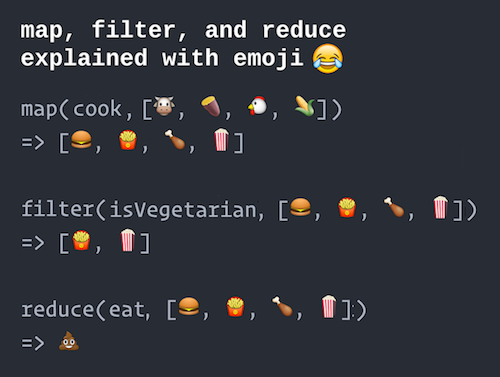
\includegraphics{imgs/07-img/map-filter-reduce-in-emoji-python.png}
\caption{Map, filter, reduce explained with emoji}
\end{figure}

All together, the \textbf{map}, \textbf{filter}, and \textbf{reduce}
operations form the basic for a functional consideration of a program.
Indeed, these kinds of operations are very common when discussing data
manipulations: for example, the famous
\href{https://en.wikipedia.org/wiki/MapReduce}{MapReduce} model involves
``mapping'' each element through a complex function (on a different
computer no less!), and then ``reducing'' the results into a single
answer.

\hypertarget{list-comprehensions}{\section{List
Comprehensions}\label{list-comprehensions}}

While \texttt{map()} and \texttt{filter()} are effective ways of
producing new lists from old, they can be somewhat hard to read
(particularly when using anonymous lambda functions, which we often
would want to do for simple transformations). Instead, a more idomatic
and ``Pythonic'' approach (preferred by language developer Guideo van
Rossum) is to use \textbf{List Comprehensions}. A \emph{list
comprehesion} is a special syntax for doing mapping and/or filtering
operations on list using the \texttt{for} and \texttt{if} keywords you
are familiar with.

A basic list comprehension has the following syntax:

\begin{Shaded}
\begin{Highlighting}[]
\NormalTok{new_list }\OperatorTok{=}\NormalTok{ [output_expression }\ControlFlowTok{for}\NormalTok{ loop_variable }\KeywordTok{in}\NormalTok{ sequence]}
\end{Highlighting}
\end{Shaded}

For example, a list comprehsion to \textbf{map} from a list of numbers
to their squares would be:

\begin{Shaded}
\begin{Highlighting}[]
\NormalTok{numbers }\OperatorTok{=}\NormalTok{ [}\DecValTok{1}\NormalTok{,}\DecValTok{2}\NormalTok{,}\DecValTok{3}\NormalTok{,}\DecValTok{4}\NormalTok{,}\DecValTok{5}\NormalTok{]  }\CommentTok{# original list}
\NormalTok{squares }\OperatorTok{=}\NormalTok{ [n}\OperatorTok{**}\DecValTok{2} \ControlFlowTok{for}\NormalTok{ n }\KeywordTok{in}\NormalTok{ numbers]}
\BuiltInTok{print}\NormalTok{(squares)  }\CommentTok{# [1, 4, 9, 16, 25]}
\end{Highlighting}
\end{Shaded}

List comprehensions are written inside square brackets
\textbf{\texttt{{[}{]}}} and use the same \texttt{for\ ...\ in\ ...}
syntax used in for loops. However, the \emph{expession} that you would
normally \texttt{append()} to the output list when mapping (or that is
returned from an anonymous lambda function) is written \emph{before} the
\texttt{for}. This causes the above comprehension to be read as
\emph{``a list consisting of \texttt{n**2} (n squares) for each
\texttt{n} in \texttt{numbers}''}---it's almost English!

You can contrast a list comprehension with the same mapping operation
done via a loop or via a \texttt{map()} and a lambda:

\begin{Shaded}
\begin{Highlighting}[]
\CommentTok{# with a loop}
\NormalTok{squares }\OperatorTok{=}\NormalTok{ []}
\ControlFlowTok{for}\NormalTok{ n }\KeywordTok{in}\NormalTok{ numbers:}
\NormalTok{    squares.append(n}\OperatorTok{**}\DecValTok{2}\NormalTok{)  }\CommentTok{# append expression}

\CommentTok{# with a lambda}
\NormalTok{squares }\OperatorTok{=} \BuiltInTok{list}\NormalTok{(}\BuiltInTok{map}\NormalTok{(}\KeywordTok{lambda}\NormalTok{ n: n}\OperatorTok{**}\DecValTok{2}\NormalTok{, numbers))  }\CommentTok{# map with lambda}

\CommentTok{# with a list comprehesion}
\NormalTok{squares }\OperatorTok{=}\NormalTok{ [n}\OperatorTok{**}\DecValTok{2} \ControlFlowTok{for}\NormalTok{ n }\KeywordTok{in}\NormalTok{ numbers]  }\CommentTok{# map with list comprehension}
\end{Highlighting}
\end{Shaded}

Notice that all 3 versions specify a \emph{transformation expression}
(\texttt{n**2}) on a input variable (\texttt{n}). They just use
different syntax (punctuation and ordering) to specify the
transformation that should occur.

List comprehensions can also be used to \textbf{filter} values (even as
they are being mapped). This is done by specifying an \texttt{if}
filtering condition after the sequence:

\begin{Shaded}
\begin{Highlighting}[]
\NormalTok{new_list }\OperatorTok{=}\NormalTok{ [output_expression }\ControlFlowTok{for}\NormalTok{ loop_variable }\KeywordTok{in}\NormalTok{ sequence }\ControlFlowTok{if}\NormalTok{ condition]}
\end{Highlighting}
\end{Shaded}

Or as a specific example (remember: we filter for elements to
\emph{keep}!):

\begin{Shaded}
\begin{Highlighting}[]
\NormalTok{numbers }\OperatorTok{=}\NormalTok{ [}\DecValTok{2}\NormalTok{,}\DecValTok{7}\NormalTok{,}\DecValTok{1}\NormalTok{,}\DecValTok{8}\NormalTok{,}\DecValTok{3}\NormalTok{]}
\NormalTok{evens }\OperatorTok{=}\NormalTok{ [n }\ControlFlowTok{for}\NormalTok{ n }\KeywordTok{in}\NormalTok{ numbers }\ControlFlowTok{if}\NormalTok{ n}\OperatorTok{%}\DecValTok{2} \OperatorTok{==} \DecValTok{0}\NormalTok{]}
\BuiltInTok{print}\NormalTok{(evens)  }\CommentTok{# [2, 8]}
\end{Highlighting}
\end{Shaded}

This can be read as \emph{``a list consisting of \texttt{n} for each
\texttt{n} in \texttt{numbers}, but only \texttt{if}
\texttt{n\%2\ ==\ 0}''}. It is equivalent to using the \texttt{for}
loop:

\begin{Shaded}
\begin{Highlighting}[]
\NormalTok{evens }\OperatorTok{=}\NormalTok{ []}
\ControlFlowTok{for}\NormalTok{ n }\KeywordTok{in}\NormalTok{ numbers}
    \ControlFlowTok{if}\NormalTok{ n}\OperatorTok{%}\DecValTok{2} \OperatorTok{==} \DecValTok{0}\NormalTok{:  }\CommentTok{# check the filter condition}
\NormalTok{        evens.append(n)  }\CommentTok{# append the expression}
\end{Highlighting}
\end{Shaded}

Finally, it is possible to include \emph{multiple, nested} \texttt{for}
and \texttt{if} statements in a list comprehension. Each successive
\texttt{for\ ...\ in\ ...} or \texttt{if} expression is included inside
the square brackets after the output expression: This allows you to
effectively convert nested control structures into a comprehension:

\begin{Shaded}
\begin{Highlighting}[]
\NormalTok{entrees }\OperatorTok{=}\NormalTok{ [}\StringTok{"chicken"}\NormalTok{,}\StringTok{"fish"}\NormalTok{,}\StringTok{"veggies"}\NormalTok{]}
\NormalTok{sides }\OperatorTok{=}\NormalTok{ [}\StringTok{"potatoes"}\NormalTok{, }\StringTok{"veggies"}\NormalTok{]}

\CommentTok{# get all "meals" if the entree and side are not the same}
\NormalTok{meals }\OperatorTok{=}\NormalTok{ [ entree}\OperatorTok{+}\StringTok{" & "}\OperatorTok{+}\NormalTok{side }\ControlFlowTok{for}\NormalTok{ entree }\KeywordTok{in}\NormalTok{ entrees }\ControlFlowTok{for}\NormalTok{ side }\KeywordTok{in}\NormalTok{ sides }\ControlFlowTok{if}\NormalTok{ entree }\OperatorTok{!=}\NormalTok{ side]}
\BuiltInTok{print}\NormalTok{(meals)  }\CommentTok{# ['chicken & potatoes', 'chicken & veggies', 'fish & potatoes',}
              \CommentTok{#  'fish & veggies', 'veggies & potatoes']}
              \CommentTok{# note: no "veggies and veggies" !}
\end{Highlighting}
\end{Shaded}

This is equivalent to the nested loops:

\begin{Shaded}
\begin{Highlighting}[]
\NormalTok{meals }\OperatorTok{=}\NormalTok{ []}
\ControlFlowTok{for}\NormalTok{ entree }\KeywordTok{in}\NormalTok{ entrees:}
    \ControlFlowTok{for}\NormalTok{ side }\KeywordTok{in}\NormalTok{ sides:}
        \ControlFlowTok{if}\NormalTok{ entree }\OperatorTok{!=}\NormalTok{ side:}
\NormalTok{            meals.append(entree}\OperatorTok{+}\StringTok{" & "}\OperatorTok{+}\NormalTok{side)}
\end{Highlighting}
\end{Shaded}

(This \emph{almost} acts like a \textbf{reduce} operation, reducing two
lists into a single one\ldots{} but it doesn't exactly convert).

Overall, list comprehensions are considered a \emph{better, more
Pythonic} approach to functional programming. However, \texttt{map()}
\texttt{filter()} and \texttt{reduce()} functions are a more generalized
approach that can be found in multiple different languages and contexts,
including other data-processing languages such as R, Julia, and
JavaScript. Thus it is good to be at least familiar with both
approaches!

\chapter{Pandas}\label{pandas}

This module introduces the \emph{Python Data Analysis} library
\href{http://pandas.pydata.org/}{\textbf{\texttt{pandas}}}---a set of
modules, functions, and classes used to for easily and efficiently
performing data analysis---\texttt{panda}'s speciality is its highly
optimized performance when working with large data sets. \texttt{pandas}
is the most common library used with Python for Data Science (and
mirrors the \texttt{R} language in many ways, allowing programmers to
easily move between the two). In this module, we will discuss the two
main data structures used by \texttt{pandas} (\emph{Series} and
\emph{DataFrames}) and how to use them to organize and work with data.

\textbf{Contents}

\begin{itemize}
\tightlist
\item
  \protect\hyperlink{resources}{Resources}
\item
  \protect\hyperlink{setup}{Setup}
\item
  \protect\hyperlink{series}{Series}
\item
  \protect\hyperlink{series-operations-and-methods}{Series Operations
  and Methods}
\item
  \protect\hyperlink{accessing-series}{Accessing Series}
\item
  \protect\hyperlink{data-frames}{Data Frames}
\item
  \protect\hyperlink{dataframe-operations-and-methods}{DataFrame
  Operations and Methods}
\item
  \protect\hyperlink{accessing-dataframes}{Accessing DataFrames}
\end{itemize}

\section{Resources}\label{resources-6}

\begin{itemize}
\tightlist
\item
  \href{http://pandas.pydata.org/pandas-docs/stable/10min.html}{10
  minutes to pandas (pandas docs)} a basic set of examples
\item
  \href{http://pandas.pydata.org/pandas-docs/stable/tutorials.html}{Tutorials
  (pandas docs)} a list and guide to various tutorials (of mixed
  quality)
\item
  \href{http://pandas.pydata.org/pandas-docs/stable/dsintro.html}{Intro
  to Data Structure (pandas docs)}
\item
  \href{http://pandas.pydata.org/pandas-docs/stable/basics.html}{Essential
  Basic Functionality (pandas docs)} not really basic, but a complete
  set of examples
\item
  \href{http://dataanalysispython.readthedocs.io/en/latest/pandas.html}{Pandas.
  Data Processing (Data Analysis in Python)}
\item
  \href{https://www.datacamp.com/courses/pandas-foundations/}{pandas
  Foundations (DataCamp)}
\end{itemize}

\hypertarget{setup}{\section{Setup}\label{setup}}

\texttt{pandas} is a \textbf{third-party} library (not built into
Python!), but is included by default with Anaconda and so can be
imported directly. Additionally, Pandas is built on top of the
\href{http://www.numpy.org/}{\texttt{numpy}} scientific computing
library which supports highly optimized mathematical operations. Thus
many \texttt{pandas} operations involve working with \texttt{numpy} data
structures, and the \texttt{pandas} library requires \texttt{numpy}
(also included in Anaconda) to also be imported:

\begin{Shaded}
\begin{Highlighting}[]
\CommentTok{# import libraries}
\ImportTok{import}\NormalTok{ pandas }\ImportTok{as}\NormalTok{ pd  }\CommentTok{# standard shortcut names}
\ImportTok{import}\NormalTok{ numpy }\ImportTok{as}\NormalTok{ np}
\end{Highlighting}
\end{Shaded}

\begin{itemize}
\item
  We usually \texttt{import} the module and reference types and methods
  using dot notation, rather than importing them into the global
  namespace.
\item
  Note that this module will focus primarily on \texttt{pandas}, leaving
  \texttt{numpy}-specific data structures and functions for the reader
  to explore.
\end{itemize}

\hypertarget{series}{\section{Series}\label{series}}

The first basic \texttt{pandas} data structure is a
\href{http://pandas.pydata.org/pandas-docs/stable/generated/pandas.Series.html}{\textbf{Series}}.
A Series represents a \emph{one-dimensional ordered collection of
values}, making them somewhat similar to a regular Python \emph{list}.
However, elements can also be given \emph{labels} (called the
\textbf{index}), which can be non-numeric values, similar to a
\emph{key} in a Python \emph{dictionary}. This makes a Series somewhat
like an ordered dictionary---one that supports additional methods and
efficient data-processing behaviors.

Series can be created using the \texttt{Series()} function (a
\emph{constructor} for instances of the class):

\begin{Shaded}
\begin{Highlighting}[]
\CommentTok{# create a Series from a list}
\NormalTok{number_series }\OperatorTok{=}\NormalTok{ pd.Series([}\DecValTok{1}\NormalTok{, }\DecValTok{2}\NormalTok{, }\DecValTok{2}\NormalTok{, }\DecValTok{3}\NormalTok{, }\DecValTok{5}\NormalTok{, }\DecValTok{8}\NormalTok{])}
\BuiltInTok{print}\NormalTok{(number_series)}
\end{Highlighting}
\end{Shaded}

produces

\begin{verbatim}
0    1
1    2
2    2
3    3
4    5
5    8
dtype: int64
\end{verbatim}

Printing a Series will display it like a \emph{table}: the first value
in each row is the \textbf{index} (label) of that element, and the
second is the value of the element in the Series.

\begin{itemize}
\tightlist
\item
  Printing will also display the \emph{type} of the elements in the
  Series. All elements in the Series will be treated as ``same''
  type---if you create a Series from mixed elements (e.g., numbers and
  strings), the type will be the a generic \texttt{object}. In practice,
  we almost always create Series from a single type.
\end{itemize}

If we create a Series from a list, each element will be given an
\emph{index} (label) that is that values's index in the list. We can
also create a Series from a \emph{dictionary}, in which case the keys
will be used as the index labels:

\begin{Shaded}
\begin{Highlighting}[]
\CommentTok{# create a Series from a dictionary}
\NormalTok{age_series }\OperatorTok{=}\NormalTok{ pd.Series(\{}\StringTok{'sarah'}\NormalTok{:}\DecValTok{42}\NormalTok{, }\StringTok{'amit'}\NormalTok{:}\DecValTok{35}\NormalTok{, }\StringTok{'zhang'}\NormalTok{:}\DecValTok{13}\NormalTok{\})}
\BuiltInTok{print}\NormalTok{(age_series)}
\end{Highlighting}
\end{Shaded}

\begin{verbatim}
amit     35
sarah    42
zhang    13
dtype: int64
\end{verbatim}

\begin{itemize}
\tightlist
\item
  Note that the Series is automatically \textbf{sorted} by the keys of
  the dictionary! This means that the order of the elements in the
  Series will always be the same for a given dictionary (which cannot be
  said for the dictionary items themselves).
\end{itemize}

\hypertarget{series-operations-and-methods}{\subsection{Series
Operations and Methods}\label{series-operations-and-methods}}

The main benefit of Series (as opposed to normal lists or dictionaries)
is that they provide a number of operations and methods that make it
easy to consider and modify the entire Series, rather than needing to
worth with each element individually. In a way, the functions include
built-in \emph{mapping}, \emph{reducing}, and \emph{filtering} style
operations.

In particular, basic operators (whether math operators such as
\texttt{+} and \texttt{-}, or relational operators such as
\texttt{\textgreater{}} or \texttt{==}) function as \textbf{vectorized
operations}, meaning that they are applied to the entire Series
\textbf{member-wise}: the operation is applied to the first element in
the Series, then the second, then the third, and so forth:

\begin{Shaded}
\begin{Highlighting}[]
\NormalTok{sample }\OperatorTok{=}\NormalTok{ pd.Series(}\BuiltInTok{range}\NormalTok{(}\DecValTok{1}\NormalTok{,}\DecValTok{6}\NormalTok{))  }\CommentTok{# Series of numbers from 1 to 5 (6 is excluded)}
\NormalTok{result }\OperatorTok{=}\NormalTok{ sample }\OperatorTok{+} \DecValTok{4}  \CommentTok{# add 4 to each element (produces new Series)}
\BuiltInTok{print}\NormalTok{(result)}
    \CommentTok{# 0    5}
    \CommentTok{# 1    6}
    \CommentTok{# 2    7}
    \CommentTok{# 3    8}
    \CommentTok{# 4    9}
    \CommentTok{# dtype: int64}

\NormalTok{is_greater_than_3 }\OperatorTok{=}\NormalTok{ sample }\OperatorTok{>} \DecValTok{3}  \CommentTok{# compare each element}
\BuiltInTok{print}\NormalTok{(is_greater_than_3)}
    \CommentTok{# 0    False}
    \CommentTok{# 1    False}
    \CommentTok{# 2    False}
    \CommentTok{# 3     True  # note index and value are not the same}
    \CommentTok{# 4     True}
    \CommentTok{# dtype: bool}
\end{Highlighting}
\end{Shaded}

\begin{itemize}
\tightlist
\item
  Having a Series operation apply to a \emph{scalar} (a single value) is
  referred to as
  \href{https://docs.scipy.org/doc/numpy/user/basics.broadcasting.html}{\textbf{broadcasting}}.
  The idea is that the smaller ``set'' of elements (e.g., a single
  value) is \emph{broadcast} so that it has a comparible size, thereby
  allowing different ``sized'' data structures to interact. Technically,
  operating on a Series with a \emph{scalar} is actually a specific case
  of operating on it with another Series!
\end{itemize}

If the second operand is \emph{another Series}, then mathematical and
relational operations are still applied \textbf{member-wise}, with the
elements of each operand being ``matched'' by their index label. This
means that for most Series whose indices are

\begin{Shaded}
\begin{Highlighting}[]
\NormalTok{s1 }\OperatorTok{=}\NormalTok{ pd.Series([}\DecValTok{2}\NormalTok{, }\DecValTok{2}\NormalTok{, }\DecValTok{2}\NormalTok{, }\DecValTok{2}\NormalTok{, }\DecValTok{2}\NormalTok{])}
\NormalTok{s2 }\OperatorTok{=}\NormalTok{ pd.Series([}\DecValTok{1}\NormalTok{, }\DecValTok{2}\NormalTok{, }\DecValTok{3}\NormalTok{, }\DecValTok{4}\NormalTok{, }\DecValTok{5}\NormalTok{])}

\CommentTok{# examples of operations (list only includes values)}
\BuiltInTok{list}\NormalTok{(s1 }\OperatorTok{+}\NormalTok{ s2)  }\CommentTok{# [3, 4, 5, 6, 7]}
\BuiltInTok{list}\NormalTok{(s1 }\OperatorTok{/}\NormalTok{ s2)  }\CommentTok{# [2.0, 1.0, 0.66666666666666663, 0.5, 0.40000000000000002]}
\BuiltInTok{list}\NormalTok{(s1 }\OperatorTok{<}\NormalTok{ s2)  }\CommentTok{# [False, False, True, True, True]}

\CommentTok{# add a Series to itself (why not?)}
\BuiltInTok{list}\NormalTok{(s2 }\OperatorTok{+}\NormalTok{ s2)  }\CommentTok{# [2, 4, 6, 8, 10]}

\CommentTok{# perform more advanced arithmetic!}
\NormalTok{s3 }\OperatorTok{=}\NormalTok{ (s1 }\OperatorTok{+}\NormalTok{ s2) }\OperatorTok{/}\NormalTok{ (s1 }\OperatorTok{+}\NormalTok{ s1)}
\BuiltInTok{list}\NormalTok{(s3)  }\CommentTok{# [0.75, 1.0, 1.25, 1.5, 1.75]}
\end{Highlighting}
\end{Shaded}

And note that these operations will be \emph{fast}, even for very large
Series, allowing for effective data manipulations.

\texttt{pandas} Series also include a number of
\href{http://pandas.pydata.org/pandas-docs/stable/generated/pandas.Series.html}{\emph{methods}}
for inspecting and manipulating the data. Some useful examples (not
comprehensive):

\begin{longtable}[]{@{}ll@{}}
\toprule
\begin{minipage}[b]{0.05\columnwidth}\raggedright\strut
Function\strut
\end{minipage} & \begin{minipage}[b]{0.05\columnwidth}\raggedright\strut
Description\strut
\end{minipage}\tabularnewline
\midrule
\endhead
\begin{minipage}[t]{0.05\columnwidth}\raggedright\strut
\texttt{index}\strut
\end{minipage} & \begin{minipage}[t]{0.05\columnwidth}\raggedright\strut
an \emph{attribute}; the sequence of index labels (convert to a
\emph{list} to use)\strut
\end{minipage}\tabularnewline
\begin{minipage}[t]{0.05\columnwidth}\raggedright\strut
\texttt{head(n)}\strut
\end{minipage} & \begin{minipage}[t]{0.05\columnwidth}\raggedright\strut
returns a Series containing only the first \texttt{n} elements\strut
\end{minipage}\tabularnewline
\begin{minipage}[t]{0.05\columnwidth}\raggedright\strut
\texttt{tail(n)}\strut
\end{minipage} & \begin{minipage}[t]{0.05\columnwidth}\raggedright\strut
returns a Series containing only the last \texttt{n} elements\strut
\end{minipage}\tabularnewline
\begin{minipage}[t]{0.05\columnwidth}\raggedright\strut
\texttt{any()}\strut
\end{minipage} & \begin{minipage}[t]{0.05\columnwidth}\raggedright\strut
returns whether ANY of the elements are \texttt{True} (or
``truthy'')\strut
\end{minipage}\tabularnewline
\begin{minipage}[t]{0.05\columnwidth}\raggedright\strut
\texttt{all()}\strut
\end{minipage} & \begin{minipage}[t]{0.05\columnwidth}\raggedright\strut
returns whether ALL of the elements are \texttt{True} (or
``truthy'')\strut
\end{minipage}\tabularnewline
\begin{minipage}[t]{0.05\columnwidth}\raggedright\strut
\texttt{mean()}\strut
\end{minipage} & \begin{minipage}[t]{0.05\columnwidth}\raggedright\strut
returns the statistical mean of the elements in the Series\strut
\end{minipage}\tabularnewline
\begin{minipage}[t]{0.05\columnwidth}\raggedright\strut
\texttt{std()}\strut
\end{minipage} & \begin{minipage}[t]{0.05\columnwidth}\raggedright\strut
returns the standard deviation of the elements in the Series\strut
\end{minipage}\tabularnewline
\begin{minipage}[t]{0.05\columnwidth}\raggedright\strut
\texttt{describe()}\strut
\end{minipage} & \begin{minipage}[t]{0.05\columnwidth}\raggedright\strut
returns a Series of
\href{http://pandas.pydata.org/pandas-docs/stable/basics.html\#descriptive-statistics}{descriptive
statistics}\strut
\end{minipage}\tabularnewline
\begin{minipage}[t]{0.05\columnwidth}\raggedright\strut
\texttt{idxmax()}\strut
\end{minipage} & \begin{minipage}[t]{0.05\columnwidth}\raggedright\strut
returns the index label of the element with the max value\strut
\end{minipage}\tabularnewline
\bottomrule
\end{longtable}

Series support many more methods as well: see the
\href{http://pandas.pydata.org/pandas-docs/stable/generated/pandas.Series.html}{full
documentation} for a complete list.

One particularly useful method to mention is the
\href{http://pandas.pydata.org/pandas-docs/stable/generated/pandas.Series.apply.html\#pandas.Series.apply}{\texttt{apply()}}
method. This method is used to \emph{apply} a particular
\textbf{callback function} to each element in the series. This is a
\emph{mapping} operation, similar to what we've done with the
\texttt{map()} function:

\begin{Shaded}
\begin{Highlighting}[]
\KeywordTok{def}\NormalTok{ square(n):  }\CommentTok{# a function that squares a number}
    \ControlFlowTok{return}\NormalTok{ n}\OperatorTok{**}\DecValTok{2}

\NormalTok{number_series }\OperatorTok{=}\NormalTok{ pd.Series([}\DecValTok{1}\NormalTok{,}\DecValTok{2}\NormalTok{,}\DecValTok{3}\NormalTok{,}\DecValTok{4}\NormalTok{,}\DecValTok{5}\NormalTok{])  }\CommentTok{# an initial series}

\NormalTok{square_series }\OperatorTok{=}\NormalTok{ number_series.}\BuiltInTok{apply}\NormalTok{(square)}
\BuiltInTok{list}\NormalTok{(square_series)  }\CommentTok{# [1, 4, 9, 16, 25]}

\CommentTok{# can also apply built-in functions}
\ImportTok{import}\NormalTok{ math}
\NormalTok{sqrt_series }\OperatorTok{=}\NormalTok{ number_series.}\BuiltInTok{apply}\NormalTok{(math.sqrt)}
\BuiltInTok{list}\NormalTok{(sqrt_series)  }\CommentTok{# [1.0, 1.4142135623730951, 1.7320508075688772, 2.0, 2.2360679774997898]}

\CommentTok{# pass additional arguments as keyword args (or `args` for a single argument)}
\NormalTok{cubed_series }\OperatorTok{=}\NormalTok{ number_series.}\BuiltInTok{apply}\NormalTok{(math.}\BuiltInTok{pow}\NormalTok{, args}\OperatorTok{=}\NormalTok{(}\DecValTok{3}\NormalTok{,)) }\CommentTok{# call math.exp(n, 3) on each}
\BuiltInTok{list}\NormalTok{(cubed_series)  }\CommentTok{# [1.0, 8.0, 27.0, 64.0, 125.0]}
\end{Highlighting}
\end{Shaded}

\hypertarget{accessing-series}{\subsection{Accessing
Series}\label{accessing-series}}

Just like lists and dictionaries, elements in a Series can be accessed
using \textbf{bracket notation}, putting the index label inside the
brackets:

\begin{Shaded}
\begin{Highlighting}[]
\NormalTok{number_series }\OperatorTok{=}\NormalTok{ pd.Series([}\DecValTok{1}\NormalTok{, }\DecValTok{2}\NormalTok{, }\DecValTok{2}\NormalTok{, }\DecValTok{3}\NormalTok{, }\DecValTok{5}\NormalTok{, }\DecValTok{8}\NormalTok{])}
\NormalTok{age_series }\OperatorTok{=}\NormalTok{ pd.Series(\{}\StringTok{'sarah'}\NormalTok{:}\DecValTok{42}\NormalTok{, }\StringTok{'amit'}\NormalTok{:}\DecValTok{35}\NormalTok{, }\StringTok{'zhang'}\NormalTok{:}\DecValTok{13}\NormalTok{\})}

\CommentTok{# get the 1th element from the number_series}
\NormalTok{number_series[}\DecValTok{1}\NormalTok{]  }\CommentTok{# 2}

\CommentTok{# get the 'sarah' element from age_series}
\NormalTok{age_series[}\StringTok{'amit'}\NormalTok{]  }\CommentTok{# 35}

\CommentTok{# get the 0th element from age_series}
\CommentTok{# (Series are ordered, so can be accessed positionally)}
\NormalTok{age_series[}\DecValTok{0}\NormalTok{]  }\CommentTok{# 42}
\end{Highlighting}
\end{Shaded}

Note that the returned values are not technically basic \texttt{int} or
\texttt{float} or \texttt{string} types, but are rather specific
\texttt{numpy} objects that work almost identically to their normal type
(but with some additional optimization).

You can also use list-style \emph{slices} using the colon operator
(e.g., elements \textbf{\texttt{1:3}}).

it is also possible to specify \textbf{\emph{a sequence of indicies}}
(i.e., a \emph{list} or \emph{range} or even a \emph{Series} of indices)
to access using bracket notation. This will produce a new Series object
that contains only the elements that have those labels:

\begin{Shaded}
\begin{Highlighting}[]
\NormalTok{age_series }\OperatorTok{=}\NormalTok{ pd.Series(\{}\StringTok{'sarah'}\NormalTok{:}\DecValTok{42}\NormalTok{, }\StringTok{'amit'}\NormalTok{:}\DecValTok{35}\NormalTok{, }\StringTok{'zhang'}\NormalTok{:}\DecValTok{13}\NormalTok{\})}

\NormalTok{index_list }\OperatorTok{=}\NormalTok{ [}\StringTok{'sarah'}\NormalTok{, }\StringTok{'zhang'}\NormalTok{]}
\BuiltInTok{print}\NormalTok{( age_series[index_list] )}
    \CommentTok{# sarah    42}
    \CommentTok{# zhang    13}
    \CommentTok{# dtype: int64}

\CommentTok{# using an anonymous variable for the index list (notice the brackets!)}
\BuiltInTok{print}\NormalTok{( age_series[[}\StringTok{'sarah'}\NormalTok{, }\StringTok{'zhang'}\NormalTok{]] )}
    \CommentTok{# sarah    42}
    \CommentTok{# zhang    13}
    \CommentTok{# dtype: int64}
\end{Highlighting}
\end{Shaded}

This also means that you can use something like a \emph{list
comprehension} to (or even a Series operation!) to determine which
elements to select from a Series!

\begin{Shaded}
\begin{Highlighting}[]
\NormalTok{letter_series }\OperatorTok{=}\NormalTok{ pd.Series([}\StringTok{'a'}\NormalTok{,}\StringTok{'b'}\NormalTok{,}\StringTok{'c'}\NormalTok{,}\StringTok{'d'}\NormalTok{,}\StringTok{'e'}\NormalTok{,}\StringTok{'f'}\NormalTok{])}
\NormalTok{even_numbers }\OperatorTok{=}\NormalTok{ [num }\ControlFlowTok{for}\NormalTok{ num }\KeywordTok{in} \BuiltInTok{range}\NormalTok{(}\DecValTok{0}\NormalTok{,}\DecValTok{6}\NormalTok{) }\ControlFlowTok{if}\NormalTok{ num}\OperatorTok{%}\DecValTok{2} \OperatorTok{==} \DecValTok{0}\NormalTok{]  }\CommentTok{# list of even numbers}

\CommentTok{# get letters with even numbered indices}
\NormalTok{letter_series[even_numbers]  }\CommentTok{# []}
    \CommentTok{# 0    a}
    \CommentTok{# 2    c}
    \CommentTok{# 4    e}
    \CommentTok{# dtype: object}

\CommentTok{# in one line (check the brackets!)}
\NormalTok{letter_series[[num }\ControlFlowTok{for}\NormalTok{ num }\KeywordTok{in} \BuiltInTok{range}\NormalTok{(}\DecValTok{0}\NormalTok{,}\DecValTok{6}\NormalTok{) }\ControlFlowTok{if}\NormalTok{ num}\OperatorTok{%}\DecValTok{2} \OperatorTok{==} \DecValTok{0}\NormalTok{]]}
\end{Highlighting}
\end{Shaded}

Finally, using a \textbf{\emph{sequence of booleans}} with bracket
notatoin will produce a new Series containing the elements whose
position \emph{corresponds} with \texttt{True} values. This is called
\textbf{boolean indexing}.

\begin{Shaded}
\begin{Highlighting}[]
\NormalTok{shoe_sizes }\OperatorTok{=}\NormalTok{ pd.Series([}\DecValTok{7}\NormalTok{, }\FloatTok{6.5}\NormalTok{, }\DecValTok{4}\NormalTok{, }\DecValTok{11}\NormalTok{, }\DecValTok{8}\NormalTok{])  }\CommentTok{# a series of shoe sizes}
\NormalTok{index_filter }\OperatorTok{=}\NormalTok{ [}\VariableTok{True}\NormalTok{, }\VariableTok{False}\NormalTok{, }\VariableTok{False}\NormalTok{, }\VariableTok{True}\NormalTok{, }\VariableTok{True}\NormalTok{]  }\CommentTok{# list of which elements to extract}

\CommentTok{# extract every element in an index that is True}
\NormalTok{shoe_sizes[index_filter]  }\CommentTok{# has values 7.0, 11.0, 8.0}
\end{Highlighting}
\end{Shaded}

\begin{itemize}
\tightlist
\item
  In this example, since \texttt{index\_filter} is \texttt{True} at
  index 0, 3, and 4, then \texttt{shoe\_sizes{[}index\_filter{]}}
  returns a Series with the elements from index numbers 0, 3, and 4.
\end{itemize}

This is incredibly powerful because it allows us to easily perform
\textbf{filtering} operations on a Series:

\begin{Shaded}
\begin{Highlighting}[]
\NormalTok{shoe_sizes }\OperatorTok{=}\NormalTok{ pd.Series([}\DecValTok{7}\NormalTok{, }\FloatTok{6.5}\NormalTok{, }\DecValTok{4}\NormalTok{, }\DecValTok{11}\NormalTok{, }\DecValTok{8}\NormalTok{])  }\CommentTok{# a series of shoe sizes}
\NormalTok{big_sizes }\OperatorTok{=}\NormalTok{ shoe_sizes }\OperatorTok{>} \FloatTok{6.5}  \CommentTok{# has values True, False, False, True, True}

\NormalTok{big_shoes }\OperatorTok{=}\NormalTok{ shoe_sizes[big_sizes]  }\CommentTok{# has values 7, 11, 8}

\CommentTok{# as one line}
\NormalTok{big_shoes }\OperatorTok{=}\NormalTok{ shoe_sizes[shoe_size }\OperatorTok{>} \FloatTok{6.5}\NormalTok{]}
\end{Highlighting}
\end{Shaded}

\begin{itemize}
\item
  You can think of the last statement as saying \emph{shoe sizes
  \textbf{where} shoe size is greater than 6.5}.
\item
  You can include \emph{logical operators} (``and'' and ``or'') by using
  the operators \texttt{\&} for ``and'' and \texttt{\textbar{}} for
  ``or''. Be sure to wrap each relational expression in \texttt{()} to
  enforce order of operations.
\end{itemize}

While it is perfectly possible to do similar filtering with a list
comprehension, the boolean indexing expression can be very simple to
read and runs quickly. (This is also the normal style of doing filtering
in the \texttt{R} programming language).

\hypertarget{data-frames}{\section{Data Frames}\label{data-frames}}

The most common data structure used in \texttt{pandas} (more common than
Series) is a
\href{http://pandas.pydata.org/pandas-docs/stable/generated/pandas.DataFrame.html}{\textbf{DataFrame}}.
A DataFrame represents a \textbf{table}, where data is organized into
rows and columns. You can think of a DataFrame as being like a Excel
spreadsheet or a SQL table.

\begin{itemize}
\tightlist
\item
  We have previously represented tabular data using a \emph{list of
  dictionaries}. However, this required us to be careful to make sure
  that all of the dictionaries shared keys, and did not offer easy ways
  to interact with the table in terms of its rows or columns. DataFrames
  give us that functionality!
\end{itemize}

A DataFrame can also be understood as a \emph{dictionary of Series},
where each Series represents a \textbf{column} of the table. The keys of
this dictionary are the \emph{index labels} of the columns, while the
the index labels of the Series serve as the labels for the row.

\begin{itemize}
\tightlist
\item
  This is distinct from spreadsheets or SQL tables, which are often seen
  as a collection of \emph{observations} (rows). Programmatically,
  DataFrames should primarily be considered as a collection of
  \emph{features} (columns), which happen to be sequenced to correspond
  to observations.
\end{itemize}

A DataFrame can be created using the \texttt{DataFrame()} function (a
\emph{constructor} for instances of the class). This function usually
takes as an argument \emph{dictionary} where the values are Series (or
values that can be converted into a Series, such as a list or a
dictionary):

\begin{Shaded}
\begin{Highlighting}[]
\NormalTok{name_series }\OperatorTok{=}\NormalTok{ pd.Series([}\StringTok{'Ada'}\NormalTok{,}\StringTok{'Bob'}\NormalTok{,}\StringTok{'Chris'}\NormalTok{,}\StringTok{'Diya'}\NormalTok{,}\StringTok{'Emma'}\NormalTok{])}
\NormalTok{heights }\OperatorTok{=} \BuiltInTok{range}\NormalTok{(}\DecValTok{58}\NormalTok{,}\DecValTok{63}\NormalTok{)}
\NormalTok{weights }\OperatorTok{=}\NormalTok{ [}\DecValTok{115}\NormalTok{, }\DecValTok{117}\NormalTok{, }\DecValTok{120}\NormalTok{, }\DecValTok{123}\NormalTok{, }\DecValTok{126}\NormalTok{]}

\NormalTok{df }\OperatorTok{=}\NormalTok{ pd.DataFrame(\{}\StringTok{'name'}\NormalTok{:name_series, }\StringTok{'height'}\NormalTok{:heights, }\StringTok{'weight'}\NormalTok{:weights\})}
\BuiltInTok{print}\NormalTok{(df)}
    \CommentTok{#    height   name  weight}
    \CommentTok{# 0      58    Ada     115}
    \CommentTok{# 1      59    Bob     117}
    \CommentTok{# 2      60  Chris     120}
    \CommentTok{# 3      61   Diya     123}
    \CommentTok{# 4      62   Emma     126}
\end{Highlighting}
\end{Shaded}

\begin{itemize}
\tightlist
\item
  Although DataFrames variables are often named \texttt{df} in
  \texttt{pandas} examples, this is \textbf{\emph{not}} a good variable
  name. You should use much more descriptive names for your DataFrames
  (e.g., \texttt{person\_size\_table}) when used in actual programs.
\item
  You can specify the order of columns in the table using the
  \texttt{columns} keyword argument, and the order of the rows using the
  \texttt{index} keyword argument.
\end{itemize}

It is also possible to create a DataFrame directly from a
spreadsheet---such as from \textbf{\texttt{.csv}} file (containing
\textbf{c}omma \textbf{s}separated \textbf{v}alues) by using the
\texttt{pandas.read\_csv()} function:

\begin{Shaded}
\begin{Highlighting}[]
\NormalTok{my_dataframe }\OperatorTok{=}\NormalTok{ pd.read_csv(}\StringTok{'path/to/my/file.csv'}\NormalTok{)}
\end{Highlighting}
\end{Shaded}

See \href{http://pandas.pydata.org/pandas-docs/stable/io.html}{the IO
Tools documentation} for details and other file-reading functions.

\hypertarget{dataframe-operations-and-methods}{\subsection{DataFrame
Operations and Methods}\label{dataframe-operations-and-methods}}

Much like Series, DataFrames support a \textbf{vectorized} form of
mathematical and relational operators: when the other operand is a
\emph{scalar}, then the operation is applied member-wise to each value
in the DataFrame:

\begin{Shaded}
\begin{Highlighting}[]
\CommentTok{# data frame of test scores}
\NormalTok{test_scores }\OperatorTok{=}\NormalTok{ pd.DataFrame(\{}
    \StringTok{'math'}\NormalTok{:[}\DecValTok{91}\NormalTok{, }\DecValTok{82}\NormalTok{, }\DecValTok{93}\NormalTok{, }\DecValTok{100}\NormalTok{, }\DecValTok{78}\NormalTok{, }\DecValTok{91}\NormalTok{],}
    \StringTok{'spanish'}\NormalTok{:[}\DecValTok{88}\NormalTok{, }\DecValTok{79}\NormalTok{, }\DecValTok{77}\NormalTok{, }\DecValTok{99}\NormalTok{, }\DecValTok{88}\NormalTok{, }\DecValTok{93}\NormalTok{]}
\NormalTok{\})}

\NormalTok{curved_scores }\OperatorTok{=}\NormalTok{ test_scores }\OperatorTok{*} \FloatTok{1.02}  \CommentTok{# curve scores up by 2%}
\BuiltInTok{print}\NormalTok{(curved_scores)}
    \CommentTok{#      math  spanish}
    \CommentTok{# 0   92.82    89.76}
    \CommentTok{# 1   83.64    80.58}
    \CommentTok{# 2   94.86    78.54}
    \CommentTok{# 3  102.00   100.98}
    \CommentTok{# 4   79.56    89.76}
    \CommentTok{# 5   92.82    94.86}

\BuiltInTok{print}\NormalTok{(curved_scores }\OperatorTok{>} \DecValTok{90}\NormalTok{)}
    \CommentTok{#     math spanish}
    \CommentTok{# 0   True   False}
    \CommentTok{# 1  False   False}
    \CommentTok{# 2   True   False}
    \CommentTok{# 3   True    True}
    \CommentTok{# 4  False   False}
    \CommentTok{# 5   True    True}
\end{Highlighting}
\end{Shaded}

It is possible to have both operands be DataFrames. In thiis case the
operation is applied member-wise, where values are matched if they have
the same row and column label. Note that any value that doesn't have a
pair will instead produce the value \texttt{NaN} (Not a Number). This is
not a normal way of working with DataFrames---it is much more common to
access individual rows and columns and work with those (e.g., add make a
new column that is the sum of two others); see below for details.

Also like Series, DataFrames objects support a large number of methods,
including:

\begin{longtable}[]{@{}ll@{}}
\toprule
\begin{minipage}[b]{0.05\columnwidth}\raggedright\strut
Function\strut
\end{minipage} & \begin{minipage}[b]{0.05\columnwidth}\raggedright\strut
Description\strut
\end{minipage}\tabularnewline
\midrule
\endhead
\begin{minipage}[t]{0.05\columnwidth}\raggedright\strut
\texttt{index}\strut
\end{minipage} & \begin{minipage}[t]{0.05\columnwidth}\raggedright\strut
an \emph{attribute}; the sequence of \textbf{row} index labels (convert
to a \emph{list} to use)\strut
\end{minipage}\tabularnewline
\begin{minipage}[t]{0.05\columnwidth}\raggedright\strut
\texttt{columns}\strut
\end{minipage} & \begin{minipage}[t]{0.05\columnwidth}\raggedright\strut
an \emph{attribute}; the sequence of \textbf{column} index labels
(convert to a \emph{list} to use)\strut
\end{minipage}\tabularnewline
\begin{minipage}[t]{0.05\columnwidth}\raggedright\strut
\texttt{head(n)}\strut
\end{minipage} & \begin{minipage}[t]{0.05\columnwidth}\raggedright\strut
returns a DataFrame containing only the first \texttt{n}
\emph{rows}\strut
\end{minipage}\tabularnewline
\begin{minipage}[t]{0.05\columnwidth}\raggedright\strut
\texttt{tail(n)}\strut
\end{minipage} & \begin{minipage}[t]{0.05\columnwidth}\raggedright\strut
returns a DataFrame containing only the last \texttt{n}
\emph{rows}\strut
\end{minipage}\tabularnewline
\begin{minipage}[t]{0.05\columnwidth}\raggedright\strut
\texttt{assign(...)}\strut
\end{minipage} & \begin{minipage}[t]{0.05\columnwidth}\raggedright\strut
returns a new DataFrame with an additional column; call as
\texttt{df.assign(new\_label=new\_column)}\strut
\end{minipage}\tabularnewline
\begin{minipage}[t]{0.05\columnwidth}\raggedright\strut
\texttt{drop(label,\ row\_or\_col)}\strut
\end{minipage} & \begin{minipage}[t]{0.05\columnwidth}\raggedright\strut
returns a new DataFrame with the given row or column removed\strut
\end{minipage}\tabularnewline
\begin{minipage}[t]{0.05\columnwidth}\raggedright\strut
\texttt{mean()}\strut
\end{minipage} & \begin{minipage}[t]{0.05\columnwidth}\raggedright\strut
returns a Series of the statistical means of the values of each
\textbf{column}\strut
\end{minipage}\tabularnewline
\begin{minipage}[t]{0.05\columnwidth}\raggedright\strut
\texttt{all()}\strut
\end{minipage} & \begin{minipage}[t]{0.05\columnwidth}\raggedright\strut
returns a Series of whether ALL the elemnts in each \textbf{column} are
\texttt{True} (or ``truthy'')\strut
\end{minipage}\tabularnewline
\begin{minipage}[t]{0.05\columnwidth}\raggedright\strut
\texttt{describe()}\strut
\end{minipage} & \begin{minipage}[t]{0.05\columnwidth}\raggedright\strut
returns a DataFrame whose columns are Series of descriptive statistics
for each \textbf{column} in the original DataFrame\strut
\end{minipage}\tabularnewline
\bottomrule
\end{longtable}

You may notice that many of these methods (e.g., \texttt{head()},
\texttt{mean()}, \texttt{describe()}, \texttt{any()}) also exist for
Series. In fact, most every method that Series support are supported by
DataFrames as well. These methods are all applied \textbf{per column}
(not per row)---that is, calling \texttt{mean()} on a DataFrame will
calculate the \emph{mean} of \textbf{each column} in that DataFrame:

\begin{Shaded}
\begin{Highlighting}[]
\NormalTok{df }\OperatorTok{=}\NormalTok{ pd.DataFrame(\{}
    \StringTok{'name'}\NormalTok{:[}\StringTok{'Ada'}\NormalTok{,}\StringTok{'Bob'}\NormalTok{,}\StringTok{'Chris'}\NormalTok{,}\StringTok{'Diya'}\NormalTok{,}\StringTok{'Emma'}\NormalTok{],}
    \StringTok{'height'}\NormalTok{:}\BuiltInTok{range}\NormalTok{(}\DecValTok{58}\NormalTok{,}\DecValTok{63}\NormalTok{),}
    \StringTok{'weights'}\NormalTok{:[}\DecValTok{115}\NormalTok{, }\DecValTok{117}\NormalTok{, }\DecValTok{120}\NormalTok{, }\DecValTok{123}\NormalTok{, }\DecValTok{126}\NormalTok{]\})}
\NormalTok{df.mean()}
    \CommentTok{# height      60.0}
    \CommentTok{# weights    120.2}
    \CommentTok{# dtype: float64}
\end{Highlighting}
\end{Shaded}

If the Series method would return a \emph{scalar} (a single value, as
with \texttt{mean()} or \texttt{any()}), then the DataFrame method
returns a Series whose labels are the column labels, as above. If the
Series method instead would return a Series (multiple values, as with
\texttt{head()} or \texttt{describe()}), then the DataFrame method
returns a new DataFrame whose columns are each of the resulting Series:

\begin{Shaded}
\begin{Highlighting}[]
\NormalTok{df }\OperatorTok{=}\NormalTok{ pd.DataFrame(\{}
    \StringTok{'name'}\NormalTok{:[}\StringTok{'Ada'}\NormalTok{,}\StringTok{'Bob'}\NormalTok{,}\StringTok{'Chris'}\NormalTok{,}\StringTok{'Diya'}\NormalTok{,}\StringTok{'Emma'}\NormalTok{],}
    \StringTok{'height'}\NormalTok{:}\BuiltInTok{range}\NormalTok{(}\DecValTok{58}\NormalTok{,}\DecValTok{63}\NormalTok{),}
    \StringTok{'weights'}\NormalTok{:[}\DecValTok{115}\NormalTok{, }\DecValTok{117}\NormalTok{, }\DecValTok{120}\NormalTok{, }\DecValTok{123}\NormalTok{, }\DecValTok{126}\NormalTok{]\})}
\NormalTok{df.describe()}
    \CommentTok{#         height     weights}
    \CommentTok{# count   5.000000    5.000000}
    \CommentTok{# mean   60.000000  120.200000}
    \CommentTok{# std     1.581139    4.438468}
    \CommentTok{# min    58.000000  115.000000}
    \CommentTok{# 25%    59.000000  117.000000}
    \CommentTok{# 50%    60.000000  120.000000}
    \CommentTok{# 75%    61.000000  123.000000}
    \CommentTok{# max    62.000000  126.000000}
\end{Highlighting}
\end{Shaded}

\begin{itemize}
\item
  Notice that the \texttt{height} column is the result of calling
  \texttt{describe()} on the DataFrame's \texttt{height} column Series!
\item
  As a general rule: if you're expecting one value per column, you'll
  get a Series of those values; if you're expecting multiple values per
  column, you'll get a DataFrame of those values.
\item
  This also means that you can sometimes ``double-call'' methods to
  reduce them further. For example, \texttt{df.any()} returns a Series
  of whether each column contains a \texttt{True} value;
  \texttt{df.all().all()} would check if \emph{that} Series contains all
  \texttt{True} values (thus checking \emph{all} columns have all
  \texttt{True} value, i.e., the entire table is all \texttt{True}
  values).
\end{itemize}

\hypertarget{accessing-dataframes}{\subsection{Accessing
DataFrames}\label{accessing-dataframes}}

DataFrames make it possible to quickly access individual or a subset of
values, though these methods use a variety of syntax structures. For
this explanation, refer to the following sample DataFrame initially
described above:

\begin{Shaded}
\begin{Highlighting}[]
\CommentTok{# all examples in this section}
\NormalTok{df }\OperatorTok{=}\NormalTok{ pd.DataFrame(\{}
    \StringTok{'name'}\NormalTok{:[}\StringTok{'Ada'}\NormalTok{,}\StringTok{'Bob'}\NormalTok{,}\StringTok{'Chris'}\NormalTok{,}\StringTok{'Diya'}\NormalTok{,}\StringTok{'Emma'}\NormalTok{],}
    \StringTok{'height'}\NormalTok{:}\BuiltInTok{range}\NormalTok{(}\DecValTok{58}\NormalTok{,}\DecValTok{63}\NormalTok{),}
    \StringTok{'weight'}\NormalTok{:[}\DecValTok{115}\NormalTok{, }\DecValTok{117}\NormalTok{, }\DecValTok{120}\NormalTok{, }\DecValTok{123}\NormalTok{, }\DecValTok{126}\NormalTok{]}
\NormalTok{\})}

\BuiltInTok{print}\NormalTok{(df)}
    \CommentTok{#     height   name   weight}
    \CommentTok{# 0      58    Ada      115}
    \CommentTok{# 1      59    Bob      117}
    \CommentTok{# 2      60  Chris      120}
    \CommentTok{# 3      61   Diya      123}
    \CommentTok{# 4      62   Emma      126}
\end{Highlighting}
\end{Shaded}

Since DataFrames are most commonly viewed as a \emph{dictionary of
columns}, it is possible to access them as such using \textbf{bracket
notation} (using the index label of the column):

\begin{Shaded}
\begin{Highlighting}[]
\BuiltInTok{print}\NormalTok{( df[}\StringTok{'height'}\NormalTok{] )  }\CommentTok{# get height column}
    \CommentTok{# 0    58}
    \CommentTok{# 1    59}
    \CommentTok{# 2    60}
    \CommentTok{# 3    61}
    \CommentTok{# 4    62}
    \CommentTok{# Name: height, dtype: int64}
\end{Highlighting}
\end{Shaded}

However, it is often more common to refer to individual columns using
\textbf{dot notation}, treating each column as an \emph{attribute} or
\emph{property} of the DataFrame object:

\begin{Shaded}
\begin{Highlighting}[]
\CommentTok{# same results as above}
\BuiltInTok{print}\NormalTok{( df.height )  }\CommentTok{# get height column}
\end{Highlighting}
\end{Shaded}

It is also possible to select \emph{multiple} columns by using a
\emph{list} or sequence inside the \textbf{bracket notation} (similar to
selecting multiple values from a Series). This will produce a new
DataFrame (a ``sub-table'')

\begin{Shaded}
\begin{Highlighting}[]
\CommentTok{# count the brackets carefully!}
\BuiltInTok{print}\NormalTok{( df[[}\StringTok{'name'}\NormalTok{, }\StringTok{'height'}\NormalTok{]] )  }\CommentTok{# get name and height columns}

\CommentTok{# can also select multiple columns with a list of their positions}
\BuiltInTok{print}\NormalTok{( df[[}\DecValTok{1}\NormalTok{,}\DecValTok{2}\NormalTok{]] )  }\CommentTok{# get 1st (name) and 2nd (weight) columns}
\end{Highlighting}
\end{Shaded}

\begin{itemize}
\tightlist
\item
  \emph{Watch out though}! Specifying a \textbf{slice} (using a colon
  \textbf{\texttt{:}}) will actually select by \emph{row} position, not
  column position!
\end{itemize}

\texttt{python\ \ \ print(\ df{[}0:2{]}\ )\ \#\ get\ ROWS\ 0\ through\ 2\ (not\ inclusive)\ \ \ \ \ \ \ \#\ \ \ \ height\ name\ \ \ weight\ \ \ \ \ \ \ \#\ 0\ \ \ \ \ \ 58\ \ Ada\ \ \ \ \ \ 115\ \ \ \ \ \ \ \#\ 1\ \ \ \ \ \ 59\ \ Bob\ \ \ \ \ \ 117}

I do not know wherefore this inconsistency, other than ``convenience''.

Because DataFrames support multiple indexes, it is possible to use
\textbf{boolean indexing} (as with Series), allowing you to
\emph{filter} for rows based the values in their columns:

\begin{Shaded}
\begin{Highlighting}[]
\BuiltInTok{print}\NormalTok{( df[ df.height }\OperatorTok{>} \DecValTok{60}\NormalTok{ ] )}
    \CommentTok{#    height  name  weight}
    \CommentTok{# 3      61  Diya     123}
    \CommentTok{# 4      62  Emma     126}
\end{Highlighting}
\end{Shaded}

\begin{itemize}
\tightlist
\item
  Note that \texttt{df.height}is a Series (a column), so
  \texttt{df.height\ \textgreater{}\ 60} produces a Series of boolean
  values (\texttt{True} and \texttt{False}). This Series is used to
  determine \emph{which} rows to return from the DataFrame---each row
  that corresponds with a \texttt{True} index.
\end{itemize}

Finally, DataFrames also provide two \emph{attributes} (properties) used
to ``quick access'' values: \textbf{\texttt{loc}}, which provides an
``index'' (lookup table) based on index labels, and
\textbf{\texttt{iloc}}, which provides an ``index'' (lookup table) based
on row and column positions. Each of these ``indexes'' can be thought of
as a \emph{dictionary} whose values are the individual elements in the
DataFrame, and whose keys can therefore be used to access those values
using \textbf{bracket notation}. The dictionaries support multiple types
of keys (using label-based \texttt{loc} as an example):

\begin{longtable}[]{@{}lll@{}}
\toprule
\begin{minipage}[b]{0.05\columnwidth}\raggedright\strut
Key Type\strut
\end{minipage} & \begin{minipage}[b]{0.05\columnwidth}\raggedright\strut
Description\strut
\end{minipage} & \begin{minipage}[b]{0.05\columnwidth}\raggedright\strut
Example\strut
\end{minipage}\tabularnewline
\midrule
\endhead
\begin{minipage}[t]{0.05\columnwidth}\raggedright\strut
\texttt{df.loc{[}row\_label{]}}\strut
\end{minipage} & \begin{minipage}[t]{0.05\columnwidth}\raggedright\strut
An individual value\strut
\end{minipage} & \begin{minipage}[t]{0.05\columnwidth}\raggedright\strut
\texttt{df.loc{[}\textquotesingle{}Ada\textquotesingle{}{]}} (the row
labeled \texttt{Ada})\strut
\end{minipage}\tabularnewline
\begin{minipage}[t]{0.05\columnwidth}\raggedright\strut
\texttt{df.loc{[}row\_label\_list{]}}\strut
\end{minipage} & \begin{minipage}[t]{0.05\columnwidth}\raggedright\strut
A list of row labels\strut
\end{minipage} & \begin{minipage}[t]{0.05\columnwidth}\raggedright\strut
\texttt{df.loc{[}{[}\textquotesingle{}Ada\textquotesingle{},\textquotesingle{}Bob\textquotesingle{}{]}{]}}
(the rows labeled \texttt{Ada} and \texttt{Bob})\strut
\end{minipage}\tabularnewline
\begin{minipage}[t]{0.05\columnwidth}\raggedright\strut
\texttt{df.loc{[}row\_label\_slice{]}}\strut
\end{minipage} & \begin{minipage}[t]{0.05\columnwidth}\raggedright\strut
A \emph{slice} of row labels\strut
\end{minipage} & \begin{minipage}[t]{0.05\columnwidth}\raggedright\strut
\texttt{df.loc{[}\textquotesingle{}Bob\textquotesingle{}:\textquotesingle{}Diya\textquotesingle{}{]}}
(the rows from \texttt{Bob} to \texttt{Diya}. Note that this is an
\emph{inclusive} slice!)\strut
\end{minipage}\tabularnewline
\begin{minipage}[t]{0.05\columnwidth}\raggedright\strut
\texttt{df.loc{[}row\_label,\ col\_label{]}}\strut
\end{minipage} & \begin{minipage}[t]{0.05\columnwidth}\raggedright\strut
A \emph{tuple} of \texttt{(row,\ column)}\strut
\end{minipage} & \begin{minipage}[t]{0.05\columnwidth}\raggedright\strut
\texttt{df.loc{[}\textquotesingle{}Ada\textquotesingle{},\ \textquotesingle{}height\textquotesingle{}{]}}
(the value at row \texttt{Ada}, column \texttt{height})\strut
\end{minipage}\tabularnewline
\begin{minipage}[t]{0.05\columnwidth}\raggedright\strut
\texttt{df.loc{[}row\_label\_seq,\ col\_label\_seq{]}}\strut
\end{minipage} & \begin{minipage}[t]{0.05\columnwidth}\raggedright\strut
A \emph{tuple} of label lists or slices\strut
\end{minipage} & \begin{minipage}[t]{0.05\columnwidth}\raggedright\strut
\texttt{df.loc{[}\textquotesingle{}Bob\textquotesingle{}:\textquotesingle{}Diya\textquotesingle{},\ {[}\textquotesingle{}height\textquotesingle{},\textquotesingle{}weight\textquotesingle{}{]}}
(the rows from \texttt{Bob} to \texttt{Diya} with the columns
\texttt{height} and \texttt{weight})\strut
\end{minipage}\tabularnewline
\bottomrule
\end{longtable}

\begin{itemize}
\item
  Note that the example \texttt{df} table doesn't have row labels beyond
  \texttt{0} to \texttt{4}
\item
  Using a \emph{tuple} makes it easy to access a particular value in the
  table, or a range of values (\emph{selecting} rows and columns ).
\item
  Note that we can also use the boundless slice \texttt{:} to refer to
  ``all elements''. So for example:
\end{itemize}

\texttt{python\ \ \ df.loc{[}:,\ \textquotesingle{}height\textquotesingle{}{]}\ \ \#\ get\ all\ rows,\ \textquotesingle{}height\textquotesingle{}\ column}

This is a basic summary of how to create and access DataFrames; for more
\href{http://pandas.pydata.org/pandas-docs/stable/basics.html\#}{detailed
usage},
\href{http://pandas.pydata.org/pandas-docs/stable/dsintro.html\#dataframe}{additional
methods}, and specific
\href{http://pandas.pydata.org/pandas-docs/stable/cookbook.html}{``recipes''},
see the
\href{http://pandas.pydata.org/pandas-docs/stable/tutorials.html}{official
\texttt{pandas} documentation}.

\bibliography{packages.bib,book.bib}


\end{document}
